\documentclass[a4paper]{book}
\usepackage{a4wide}
\usepackage{makeidx}
\usepackage{fancyhdr}
\usepackage{graphicx}
\usepackage{multicol}
\usepackage{float}
\usepackage{textcomp}
\usepackage{alltt}
\usepackage[utf8]{inputenc}
\usepackage{doxygen}
\makeindex
\setcounter{tocdepth}{1}
\renewcommand{\footrulewidth}{0.4pt}
\begin{document}
\begin{titlepage}
\vspace*{7cm}
\begin{center}
{\Large ISokoban Reference Manual\\[1ex]\large 1.0 }\\
\vspace*{1cm}
{\large Generated by Doxygen 1.5.3}\\
\vspace*{0.5cm}
{\small Sun Jun 1 18:02:05 2008}\\
\end{center}
\end{titlepage}
\clearemptydoublepage
\pagenumbering{roman}
\tableofcontents
\clearemptydoublepage
\pagenumbering{arabic}
\chapter{ISokoban Hierarchical Index}
\section{ISokoban Class Hierarchy}
This inheritance list is sorted roughly, but not completely, alphabetically:\begin{CompactList}
\item \contentsline{section}{BotA}{\pageref{classBotA}}{}
\begin{CompactList}
\item \contentsline{section}{BotBestMovesS}{\pageref{classBotBestMovesS}}{}
\end{CompactList}
\item \contentsline{section}{BotBestPushesS\_\-Penalties}{\pageref{classBotBestPushesS__Penalties}}{}
\item \contentsline{section}{BotBFS}{\pageref{classBotBFS}}{}
\item \contentsline{section}{BotDFS}{\pageref{classBotDFS}}{}
\item \contentsline{section}{BotGoodPushesS}{\pageref{classBotGoodPushesS}}{}
\item \contentsline{section}{BotIDA}{\pageref{classBotIDA}}{}
\item \contentsline{section}{CellList}{\pageref{classCellList}}{}
\item \contentsline{section}{ChainedList}{\pageref{classChainedList}}{}
\begin{CompactList}
\item \contentsline{section}{BotA\_\-ChainedList}{\pageref{classBotA__ChainedList}}{}
\item \contentsline{section}{BotA\_\-HeapStack}{\pageref{classBotA__HeapStack}}{}
\end{CompactList}
\item \contentsline{section}{Data}{\pageref{classData}}{}
\item \contentsline{section}{HashTable}{\pageref{classHashTable}}{}
\begin{CompactList}
\item \contentsline{section}{BotA\_\-HashTable}{\pageref{classBotA__HashTable}}{}
\end{CompactList}
\item \contentsline{section}{Level}{\pageref{classLevel}}{}
\item \contentsline{section}{ListNode}{\pageref{classListNode}}{}
\begin{CompactList}
\item \contentsline{section}{BotA\_\-ListNode}{\pageref{classBotA__ListNode}}{}
\item \contentsline{section}{BotA\_\-ListNode2}{\pageref{classBotA__ListNode2}}{}
\end{CompactList}
\item \contentsline{section}{Node}{\pageref{classNode}}{}
\item \contentsline{section}{Node::Macro}{\pageref{classNode_1_1Macro}}{}
\item \contentsline{section}{Pack}{\pageref{classPack}}{}
\item \contentsline{section}{Path}{\pageref{classPath}}{}
\item \contentsline{section}{StringList}{\pageref{classStringList}}{}
\item \contentsline{section}{TreeNode}{\pageref{classTreeNode}}{}
\item \contentsline{section}{Util}{\pageref{classUtil}}{}
\item \contentsline{section}{Zone}{\pageref{classZone}}{}
\end{CompactList}

\chapter{ISokoban Class Index}
\section{ISokoban Class List}
Here are the classes, structs, unions and interfaces with brief descriptions:\begin{CompactList}
\item\contentsline{section}{{\bf BotA} (A implementation of A$\ast$ algorithm without specific function f(x) = g(x) + h(x) (this class must be derived) )}{\pageref{classBotA}}{}
\item\contentsline{section}{{\bf BotA\_\-ChainedList} (A specific version of \doxyref{ChainedList}{p.}{classChainedList} to use specific listNodes with heapStackCell values (only used with closeNodeList) )}{\pageref{classBotA__ChainedList}}{}
\item\contentsline{section}{{\bf BotA\_\-HashTable} (A version of \doxyref{HashTable}{p.}{classHashTable} specific to closeNodeList in heap stack With it, we can get or change heapStackCell value of a specific node in the hashtable )}{\pageref{classBotA__HashTable}}{}
\item\contentsline{section}{{\bf BotA\_\-HeapStack} (A Heap Stack of TreeNodes. It can work like a chainedList to sort TreeNodes in order of cost. Smallest is always root treeNode of stack )}{\pageref{classBotA__HeapStack}}{}
\item\contentsline{section}{{\bf BotA\_\-ListNode} (A version of \doxyref{ListNode}{p.}{classListNode} with \char`\"{}f\char`\"{} and \char`\"{}g\char`\"{} getters where f(x)=g(x)+h(x). It's used to make the A$\ast$ solver )}{\pageref{classBotA__ListNode}}{}
\item\contentsline{section}{{\bf BotA\_\-ListNode2} (A version of \doxyref{ListNode}{p.}{classListNode} with \char`\"{}f\char`\"{} and \char`\"{}g\char`\"{} getters where f(x)=g(x)+h(x). It's used to make the A$\ast$ solver WARNING : this second version of \doxyref{ListNode}{p.}{classListNode} is dedicated to close hashtable and use one more variable : \char`\"{}heapStackCell\char`\"{}. heapStackCell is the number of cell treeNode of this Listnode is currently in )}{\pageref{classBotA__ListNode2}}{}
\item\contentsline{section}{{\bf BotBestMovesS} (A$\ast$ algorithm based on moves number of the pusher. Nodes with less moves are explored first. WARNING : this algorithm doesn't return best moves solution of this level but only a good solution. This is because a state representation of the level doesn't keep exact pusher position but only a pusher zone. This solver will work efficiently (but with a lot of extra work) only if we make level representation with boxes position (zone) and exact pusher position (integer) )}{\pageref{classBotBestMovesS}}{}
\item\contentsline{section}{{\bf BotBestPushesS\_\-Penalties} (Management of cost penalties. Try to detect every sub-states that causes a penalty to the initial cost )}{\pageref{classBotBestPushesS__Penalties}}{}
\item\contentsline{section}{{\bf BotBFS} (Breadth-first search implementation of solver )}{\pageref{classBotBFS}}{}
\item\contentsline{section}{{\bf BotDFS} (Depth-first search implementation of solver )}{\pageref{classBotDFS}}{}
\item\contentsline{section}{{\bf BotGoodPushesS} (A$\ast$ search algorithm based on estimated remaining pushes number of the pusher. (f(x) = h(x)) Nodes with less pushes are explored first. this algorithm DOESN'T return best pushes solution of this level but only a good solution )}{\pageref{classBotGoodPushesS}}{}
\item\contentsline{section}{{\bf BotIDA} (IDA$\ast$ algorithm based on best pushes number )}{\pageref{classBotIDA}}{}
\item\contentsline{section}{{\bf CellList} (Dijkstra algorithm used to see what goals a box can reach and with how many pushes it could )}{\pageref{classCellList}}{}
\item\contentsline{section}{{\bf ChainedList} (Main Double Chained List of ListNodes class )}{\pageref{classChainedList}}{}
\item\contentsline{section}{{\bf Data} (Datas relative to game context )}{\pageref{classData}}{}
\item\contentsline{section}{{\bf HashTable} (Hash Table Class to store all level states )}{\pageref{classHashTable}}{}
\item\contentsline{section}{{\bf Level} (Class containing a level and every functions about it )}{\pageref{classLevel}}{}
\item\contentsline{section}{{\bf ListNode} (\doxyref{Node}{p.}{classNode} representation for chained lists )}{\pageref{classListNode}}{}
\item\contentsline{section}{{\bf Node} (Lowest representation of a node. Only contain pusher zone and boxes zone )}{\pageref{classNode}}{}
\item\contentsline{section}{{\bf Node::Macro} }{\pageref{classNode_1_1Macro}}{}
\item\contentsline{section}{{\bf Pack} (Class used to store a (xml) pack of levels )}{\pageref{classPack}}{}
\item\contentsline{section}{{\bf Path} (Class usefull to represent a way to move in a level )}{\pageref{classPath}}{}
\item\contentsline{section}{{\bf StringList} (Management of Lists made of strings )}{\pageref{classStringList}}{}
\item\contentsline{section}{{\bf TreeNode} (Improved node representation for trees )}{\pageref{classTreeNode}}{}
\item\contentsline{section}{{\bf Util} (Utility class only with static method )}{\pageref{classUtil}}{}
\item\contentsline{section}{{\bf Zone} (Binary representation of positions in a level )}{\pageref{classZone}}{}
\end{CompactList}

\chapter{ISokoban Class Documentation}
\section{BotA Class Reference}
\label{classBotA}\index{BotA@{BotA}}
A implementation of A$\ast$ algorithm without specific function f(x) = g(x) + h(x) (this class must be derived).  


{\tt \#include $<$BotA.h$>$}

Inheritance diagram for BotA::\begin{figure}[H]
\begin{center}
\leavevmode
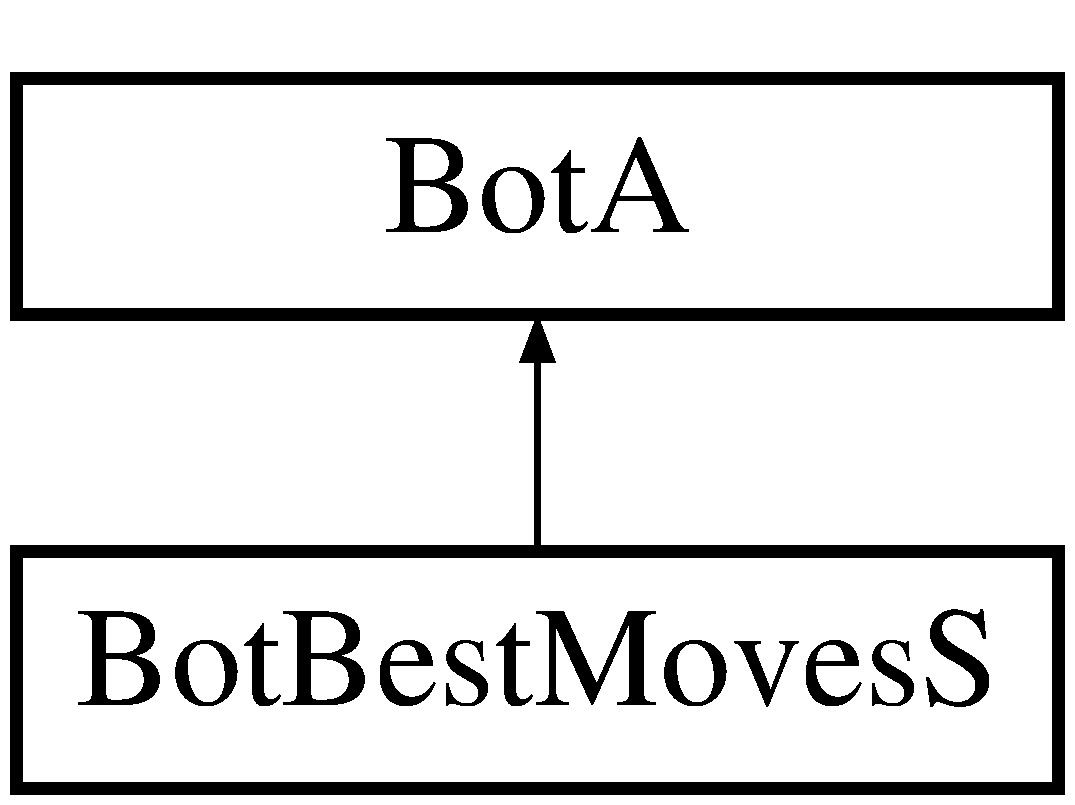
\includegraphics[height=2cm]{classBotA}
\end{center}
\end{figure}
\subsection*{Public Member Functions}
\begin{CompactItemize}
\item 
virtual const char $\ast$ {\bf SOLVER\_\-NAME} ()=0
\item 
{\bf BotA} (Base $\ast$base, {\bf Level} $\ast$level, int maxNodeNumber, int maxRamSize, int openTableSize, int closeTableSize, int {\bf costLimit}, int deadlockedBoxesSearch=2, bool onlyPushNumber=false, bool {\bf quickSearch}=false)
\item 
int {\bf getMinReject} (void) const 
\item 
int {\bf getCostLimit} (void) const 
\item 
int {\bf getQuickSearch} (void) const 
\item 
virtual int {\bf getSize} (void)
\item 
int {\bf getInitialCost} ()
\end{CompactItemize}
\subsection*{Protected Member Functions}
\begin{CompactItemize}
\item 
virtual void {\bf process} ()
\item 
void {\bf saveMostUsedPositions} (int numberOfPos)
\item 
bool {\bf isDeadTreeNode} ({\bf TreeNode} $\ast$treeNode)
\item 
void {\bf deleteDeadTreeNode} ({\bf TreeNode} $\ast$treeNode)
\item 
bool {\bf workOnAlreadySearched} ({\bf TreeNode} $\ast$treeNode, int $\ast$counter)
\item 
{\bf TreeNode} $\ast$ {\bf firstTreeNode} (void)
\item 
Child $\ast$$\ast$ {\bf findPonderedChildren} ({\bf TreeNode} $\ast$treeNode)
\item 
virtual void {\bf addTreeNodeToCloseList} ({\bf TreeNode} $\ast$treeNode)
\item 
virtual void {\bf initHashTable} (void)
\item 
virtual void {\bf initCloseNodeList} (void)
\item 
virtual {\bf TreeNode} $\ast$ {\bf createTreeNode} ({\bf Node} $\ast$node, {\bf TreeNode} $\ast$parentTreeNode, int pushCost)
\item 
void {\bf moveTreeNode} ({\bf TreeNode} $\ast$treeNode, {\bf TreeNode} $\ast$newParent)
\item 
virtual int {\bf f} ({\bf TreeNode} $\ast$treeNode, int pushCost) const =0
\item 
virtual int {\bf g} ({\bf TreeNode} $\ast$treeNode, int pushCost) const =0
\item 
virtual int {\bf h} ({\bf TreeNode} $\ast$treeNode) const =0
\item 
virtual bool {\bf testSolution} ({\bf TreeNode} $\ast$treeNode)
\item 
virtual bool {\bf solutionNode} (const {\bf TreeNode} $\ast$treeNode) const 
\item 
int $\ast$ {\bf mostUsedPositions} (int number, bool withGoals)
\item 
int {\bf findMaxCellAndReplaceValue} (int $\ast$tab, int tabLength, bool withGoals)
\item 
virtual void {\bf printInfos} ({\bf TreeNode} $\ast$treeNode)
\end{CompactItemize}
\subsection*{Protected Attributes}
\begin{CompactItemize}
\item 
int {\bf costLimit}
\item 
int {\bf minReject}
\item 
bool {\bf quickSearch}
\end{CompactItemize}


\subsection{Detailed Description}
A implementation of A$\ast$ algorithm without specific function f(x) = g(x) + h(x) (this class must be derived). 

\subsection{Constructor \& Destructor Documentation}
\index{BotA@{BotA}!BotA@{BotA}}
\index{BotA@{BotA}!BotA@{BotA}}
\subsubsection{\setlength{\rightskip}{0pt plus 5cm}BotA::BotA (Base $\ast$ {\em base}, {\bf Level} $\ast$ {\em level}, int {\em maxNodeNumber}, int {\em maxRamSize}, int {\em openTableSize}, int {\em closeTableSize}, int {\em costLimit}, int {\em deadlockedBoxesSearch} = {\tt 2}, bool {\em onlyPushNumber} = {\tt false}, bool {\em quickSearch} = {\tt false})}\label{classBotA_9445dbf366ee48d823b3a14c8a2f2ccc}


Constructor for a solver of a level \begin{Desc}
\item[Parameters:]
\begin{description}
\item[{\em base}]main class of the game \item[{\em level}]\doxyref{Level}{p.}{classLevel} to be used \item[{\em maxNodeNumber}]Limit number of nodes to explore \item[{\em maxRamSize}]Limit max ram size to allocate \item[{\em openTableSize}]size of Open Table to allocate (hashtable) \item[{\em closeTableSize}]size of Close Table to allocate (hashtable) \item[{\em limit}]of accepted f(x). if costLimit = -1, costLimit = +infinity \item[{\em deadlockedBoxesSearch}]number of boxes to use when testing every possible positions of deadlock \item[{\em onlyPushNumber}]only keep number of pushes in Stats object. don't generate solution \doxyref{Path}{p.}{classPath} (CPU saving for deadlocks and penalties) \item[{\em quickSearch}]don't test penalties of every nodes before adding it on the tree \end{description}
\end{Desc}


\subsection{Member Function Documentation}
\index{BotA@{BotA}!SOLVER_NAME@{SOLVER\_\-NAME}}
\index{SOLVER_NAME@{SOLVER\_\-NAME}!BotA@{BotA}}
\subsubsection{\setlength{\rightskip}{0pt plus 5cm}virtual const char$\ast$ BotA::SOLVER\_\-NAME ()\hspace{0.3cm}{\tt  [pure virtual]}}\label{classBotA_ab85547e677baf43658369ab19a461c4}


Name of this solver 

Implemented in {\bf BotBestMovesS} \doxyref{}{p.}{classBotBestMovesS_c29b9292fd9d234d1d4e7c8ef4e36720}.\index{BotA@{BotA}!getMinReject@{getMinReject}}
\index{getMinReject@{getMinReject}!BotA@{BotA}}
\subsubsection{\setlength{\rightskip}{0pt plus 5cm}int BotA::getMinReject (void) const\hspace{0.3cm}{\tt  [inline]}}\label{classBotA_c2684957f288ca6d0bbe8df235e73d77}


minReject \index{BotA@{BotA}!getCostLimit@{getCostLimit}}
\index{getCostLimit@{getCostLimit}!BotA@{BotA}}
\subsubsection{\setlength{\rightskip}{0pt plus 5cm}int BotA::getCostLimit (void) const\hspace{0.3cm}{\tt  [inline]}}\label{classBotA_f679b068a36cdf048dc69c03b0f0e673}


limit of accepted f(x) \index{BotA@{BotA}!getQuickSearch@{getQuickSearch}}
\index{getQuickSearch@{getQuickSearch}!BotA@{BotA}}
\subsubsection{\setlength{\rightskip}{0pt plus 5cm}int BotA::getQuickSearch (void) const\hspace{0.3cm}{\tt  [inline]}}\label{classBotA_0f2306d676e3583d56cfb487f7a1ce51}


quick search \index{BotA@{BotA}!getSize@{getSize}}
\index{getSize@{getSize}!BotA@{BotA}}
\subsubsection{\setlength{\rightskip}{0pt plus 5cm}int BotA::getSize (void)\hspace{0.3cm}{\tt  [virtual]}}\label{classBotA_d607c14485f9d5fa20fd30e30b6167a9}


Return size in octets of the actual state of this solver \begin{Desc}
\item[Returns:]size in octets of the actual state of this solver \end{Desc}
\index{BotA@{BotA}!getInitialCost@{getInitialCost}}
\index{getInitialCost@{getInitialCost}!BotA@{BotA}}
\subsubsection{\setlength{\rightskip}{0pt plus 5cm}int BotA::getInitialCost ()}\label{classBotA_0cf8ff14953027a208fc9a4b4aa3e2a6}


Get cost of first treeNode \begin{Desc}
\item[Returns:]cost of first treeNode \end{Desc}
\index{BotA@{BotA}!process@{process}}
\index{process@{process}!BotA@{BotA}}
\subsubsection{\setlength{\rightskip}{0pt plus 5cm}void BotA::process ()\hspace{0.3cm}{\tt  [protected, virtual]}}\label{classBotA_e6a4b7fbc9556cebde69fb6645e33c5e}


Try to resolve this level with a fixed max number of nodes or a fixed max number of ram size to allocate. (first to be reached) \index{BotA@{BotA}!saveMostUsedPositions@{saveMostUsedPositions}}
\index{saveMostUsedPositions@{saveMostUsedPositions}!BotA@{BotA}}
\subsubsection{\setlength{\rightskip}{0pt plus 5cm}void BotA::saveMostUsedPositions (int {\em numberOfPos})\hspace{0.3cm}{\tt  [protected]}}\label{classBotA_c261752475e178e7c24dc71971e7e052}


If ram limit or node limit are reached, we save a list of sub-states of boxes where cells are most used by boxes in the tree. This list of sub-states will be tested before next solving of same level \begin{Desc}
\item[Parameters:]
\begin{description}
\item[{\em number}]of \char`\"{}top\char`\"{} cell positions we want to keep. If we take 15, we will have list of every sub-states of 1,2,3,4,5 and 6 boxes for 15 most used positions \end{description}
\end{Desc}
\index{BotA@{BotA}!isDeadTreeNode@{isDeadTreeNode}}
\index{isDeadTreeNode@{isDeadTreeNode}!BotA@{BotA}}
\subsubsection{\setlength{\rightskip}{0pt plus 5cm}bool BotA::isDeadTreeNode ({\bf TreeNode} $\ast$ {\em treeNode})\hspace{0.3cm}{\tt  [protected]}}\label{classBotA_13af1593d0bbd3232fa3402f93d9fffd}


Test if a treenode is a dead branch (treenode and all children are in openTable) or not \begin{Desc}
\item[Parameters:]
\begin{description}
\item[{\em treeNode}]node to be tested \end{description}
\end{Desc}
\begin{Desc}
\item[Returns:]true if treenode is a dead branch, false if not \end{Desc}
\index{BotA@{BotA}!deleteDeadTreeNode@{deleteDeadTreeNode}}
\index{deleteDeadTreeNode@{deleteDeadTreeNode}!BotA@{BotA}}
\subsubsection{\setlength{\rightskip}{0pt plus 5cm}void BotA::deleteDeadTreeNode ({\bf TreeNode} $\ast$ {\em treeNode})\hspace{0.3cm}{\tt  [protected]}}\label{classBotA_0661c8a1282d795601a08cdcadecee23}


delete a dead treenode from the tree and all its children. Also delete this node from openTable. \begin{Desc}
\item[Parameters:]
\begin{description}
\item[{\em treeNode}]node to be deleted \end{description}
\end{Desc}
\index{BotA@{BotA}!workOnAlreadySearched@{workOnAlreadySearched}}
\index{workOnAlreadySearched@{workOnAlreadySearched}!BotA@{BotA}}
\subsubsection{\setlength{\rightskip}{0pt plus 5cm}bool BotA::workOnAlreadySearched ({\bf TreeNode} $\ast$ {\em treeNode}, int $\ast$ {\em counter})\hspace{0.3cm}{\tt  [protected]}}\label{classBotA_2b98a2d6a402cac989295d0e61e41c3e}


If this node is already searched, we look at the cost of stocked treeNode and move what it need to be moved to keep the lowest cost \begin{Desc}
\item[Parameters:]
\begin{description}
\item[{\em treeNode}]treenode we want to look if it's new or beter than anything existing \item[{\em counter}]counter of children of actual treeNode \end{description}
\end{Desc}
\begin{Desc}
\item[Returns:]true if it's already searched and doesn't need to be added. false if it's not already searched and we need to add it. \end{Desc}
\index{BotA@{BotA}!firstTreeNode@{firstTreeNode}}
\index{firstTreeNode@{firstTreeNode}!BotA@{BotA}}
\subsubsection{\setlength{\rightskip}{0pt plus 5cm}{\bf TreeNode} $\ast$ BotA::firstTreeNode (void)\hspace{0.3cm}{\tt  [protected]}}\label{classBotA_e2f84fb58a1a2083ddedeb0aa1be8417}


Get first treeNode from closeNodeList and delete it from the list \begin{Desc}
\item[Returns:]first treeNode from closeNodeList \end{Desc}
\index{BotA@{BotA}!findPonderedChildren@{findPonderedChildren}}
\index{findPonderedChildren@{findPonderedChildren}!BotA@{BotA}}
\subsubsection{\setlength{\rightskip}{0pt plus 5cm}Child $\ast$$\ast$ BotA::findPonderedChildren ({\bf TreeNode} $\ast$ {\em treeNode})\hspace{0.3cm}{\tt  [protected]}}\label{classBotA_d28875b477b72a8828c974db207253a7}


Get list of children from a treeNode and move this treenode from close list to open list. This function take macro children too. (children with many pushes to put a box on a goal in one step) \begin{Desc}
\item[Parameters:]
\begin{description}
\item[{\em treeNode}]treeNode we want to find children \end{description}
\end{Desc}
\begin{Desc}
\item[Returns:]list of children (terminated by NULL) with list of cost (number of push) of every children. When it's not a macro push, it's always 1. \end{Desc}
\index{BotA@{BotA}!addTreeNodeToCloseList@{addTreeNodeToCloseList}}
\index{addTreeNodeToCloseList@{addTreeNodeToCloseList}!BotA@{BotA}}
\subsubsection{\setlength{\rightskip}{0pt plus 5cm}void BotA::addTreeNodeToCloseList ({\bf TreeNode} $\ast$ {\em treeNode})\hspace{0.3cm}{\tt  [protected, virtual]}}\label{classBotA_e948f2346aaa4c84393d5ef0cfe0eb2f}


Add a new \doxyref{TreeNode}{p.}{classTreeNode} to the waiting list at the right position. New Treenode is added TO THE CORRECT PLACE DEPENDING OF ITS COST (best-first search) \index{BotA@{BotA}!initHashTable@{initHashTable}}
\index{initHashTable@{initHashTable}!BotA@{BotA}}
\subsubsection{\setlength{\rightskip}{0pt plus 5cm}void BotA::initHashTable (void)\hspace{0.3cm}{\tt  [protected, virtual]}}\label{classBotA_df50adec8741de89e6e15cba2354a85b}


Initialize empty hashtables \index{BotA@{BotA}!initCloseNodeList@{initCloseNodeList}}
\index{initCloseNodeList@{initCloseNodeList}!BotA@{BotA}}
\subsubsection{\setlength{\rightskip}{0pt plus 5cm}void BotA::initCloseNodeList (void)\hspace{0.3cm}{\tt  [protected, virtual]}}\label{classBotA_a5899fa5196b3e759df41295819a5172}


Initialize empty waiting node list \index{BotA@{BotA}!createTreeNode@{createTreeNode}}
\index{createTreeNode@{createTreeNode}!BotA@{BotA}}
\subsubsection{\setlength{\rightskip}{0pt plus 5cm}{\bf TreeNode} $\ast$ BotA::createTreeNode ({\bf Node} $\ast$ {\em node}, {\bf TreeNode} $\ast$ {\em parentTreeNode}, int {\em pushCost})\hspace{0.3cm}{\tt  [protected, virtual]}}\label{classBotA_1d03bd289e6c6f2425c29d8a8e0b3933}


Create a \doxyref{TreeNode}{p.}{classTreeNode} from a node and its parent treeNode in the search tree (if he got one, else NULL) and assign a cost at it \begin{Desc}
\item[Parameters:]
\begin{description}
\item[{\em node}]\doxyref{Node}{p.}{classNode} we want to put in the new \doxyref{TreeNode}{p.}{classTreeNode} \item[{\em parentTreeNode}]Parent \doxyref{TreeNode}{p.}{classTreeNode} we want to attach to new \doxyref{TreeNode}{p.}{classTreeNode} \item[{\em pushCost}]number of pushes from its parent (usefull for macro-pushes) \end{description}
\end{Desc}
\begin{Desc}
\item[Returns:]a new \doxyref{TreeNode}{p.}{classTreeNode} that contains param \char`\"{}Node\char`\"{} and a definied cost \end{Desc}
\index{BotA@{BotA}!moveTreeNode@{moveTreeNode}}
\index{moveTreeNode@{moveTreeNode}!BotA@{BotA}}
\subsubsection{\setlength{\rightskip}{0pt plus 5cm}void BotA::moveTreeNode ({\bf TreeNode} $\ast$ {\em treeNode}, {\bf TreeNode} $\ast$ {\em newParent})\hspace{0.3cm}{\tt  [protected]}}\label{classBotA_ad58285e1b3d2b39df61627f3b1be0bc}


Move a treenode in the tree by split it from its parent and attach it to a new parent \begin{Desc}
\item[Parameters:]
\begin{description}
\item[{\em treeNode}]treenode we want to move in the tree \item[{\em newParent}]new parent for this treenode \end{description}
\end{Desc}
\index{BotA@{BotA}!f@{f}}
\index{f@{f}!BotA@{BotA}}
\subsubsection{\setlength{\rightskip}{0pt plus 5cm}virtual int BotA::f ({\bf TreeNode} $\ast$ {\em treeNode}, int {\em pushCost}) const\hspace{0.3cm}{\tt  [protected, pure virtual]}}\label{classBotA_7f064a1906ff8150a2326a8f9d73c2f7}


Cost function to evaluate the cost of a treenode with its position in the tree (parent of treenode must be assigned before calling this function) \begin{Desc}
\item[Parameters:]
\begin{description}
\item[{\em treeNode}]to be computed \item[{\em pushCost}]number of pushes from its parent (usefull for macro-pushes) \end{description}
\end{Desc}
\begin{Desc}
\item[Returns:]cost value of this node \end{Desc}
\index{BotA@{BotA}!g@{g}}
\index{g@{g}!BotA@{BotA}}
\subsubsection{\setlength{\rightskip}{0pt plus 5cm}virtual int BotA::g ({\bf TreeNode} $\ast$ {\em treeNode}, int {\em pushCost}) const\hspace{0.3cm}{\tt  [protected, pure virtual]}}\label{classBotA_a1210833ae6accea9e659a2deb062a2a}


Cost function to evaluate the cost of getting to this treeNode from the initial treenode (parent of treenode must be assigned before calling this function) \begin{Desc}
\item[Parameters:]
\begin{description}
\item[{\em treeNode}]to be computed \item[{\em pushCost}]number of pushes from its parent (usefull for macro-pushes) \end{description}
\end{Desc}
\begin{Desc}
\item[Returns:]cost value from start to this node \end{Desc}
\index{BotA@{BotA}!h@{h}}
\index{h@{h}!BotA@{BotA}}
\subsubsection{\setlength{\rightskip}{0pt plus 5cm}virtual int BotA::h ({\bf TreeNode} $\ast$ {\em treeNode}) const\hspace{0.3cm}{\tt  [protected, pure virtual]}}\label{classBotA_c9d54cca141a1f1638a3482a616e9403}


Cost function to evaluate the cost of admissibly estimated distance to a goal treenode from this treenode (parent of treenode must be assigned before calling this function) 

Implemented in {\bf BotBestMovesS} \doxyref{}{p.}{classBotBestMovesS_737fff641aa19f3d89cf98cf87c6ba76}.\index{BotA@{BotA}!testSolution@{testSolution}}
\index{testSolution@{testSolution}!BotA@{BotA}}
\subsubsection{\setlength{\rightskip}{0pt plus 5cm}bool BotA::testSolution ({\bf TreeNode} $\ast$ {\em treeNode})\hspace{0.3cm}{\tt  [protected, virtual]}}\label{classBotA_36ac7cef4eb59696ca81ce1aee4f0131}


Test if a treeNode is a solution node and create Stats object. \begin{Desc}
\item[Parameters:]
\begin{description}
\item[{\em treeNode}]treenode we want to test \end{description}
\end{Desc}
\begin{Desc}
\item[Returns:]true if this treenode is a solution, false if not \end{Desc}
\index{BotA@{BotA}!solutionNode@{solutionNode}}
\index{solutionNode@{solutionNode}!BotA@{BotA}}
\subsubsection{\setlength{\rightskip}{0pt plus 5cm}bool BotA::solutionNode (const {\bf TreeNode} $\ast$ {\em treeNode}) const\hspace{0.3cm}{\tt  [protected, virtual]}}\label{classBotA_783294a958a9f517e653f7b3c00d0ebb}


Test if a treenode is a solution treenode (based on h(x)=0 value) \begin{Desc}
\item[Parameters:]
\begin{description}
\item[{\em treeNode}]\doxyref{TreeNode}{p.}{classTreeNode} to tested \end{description}
\end{Desc}
\begin{Desc}
\item[Returns:]true if this node is solution (h(x) = 0), false if not \end{Desc}
\index{BotA@{BotA}!mostUsedPositions@{mostUsedPositions}}
\index{mostUsedPositions@{mostUsedPositions}!BotA@{BotA}}
\subsubsection{\setlength{\rightskip}{0pt plus 5cm}int $\ast$ BotA::mostUsedPositions (int {\em number}, bool {\em withGoals})\hspace{0.3cm}{\tt  [protected]}}\label{classBotA_32c08ab7a41550f6d59a9ccdd2f405dd}


Find most used positions (boxes on them). Positions with goals or without goals. \begin{Desc}
\item[Parameters:]
\begin{description}
\item[{\em number}]number of most used positions we want to find \item[{\em withGoals}]true if we want to take care of goals, false if not \end{description}
\end{Desc}
\begin{Desc}
\item[Returns:]tab of \char`\"{}number\char`\"{} cells filled with most used positions. Be carefull, this tab can be ended with several -1 \char`\"{}number\char`\"{} is bigger than usefull cells \end{Desc}
\index{BotA@{BotA}!findMaxCellAndReplaceValue@{findMaxCellAndReplaceValue}}
\index{findMaxCellAndReplaceValue@{findMaxCellAndReplaceValue}!BotA@{BotA}}
\subsubsection{\setlength{\rightskip}{0pt plus 5cm}int BotA::findMaxCellAndReplaceValue (int $\ast$ {\em tab}, int {\em tabLength}, bool {\em withGoals})\hspace{0.3cm}{\tt  [protected]}}\label{classBotA_5a136484ea281a4d12706c6e16576b89}


find max cell of a tab, keep it, and replace it with -1 \begin{Desc}
\item[Parameters:]
\begin{description}
\item[{\em tab}]tab of values \item[{\em tabLength}]length of tab \item[{\em withGoals}]true if we want to take care of goals, false if not \end{description}
\end{Desc}
\begin{Desc}
\item[Returns:]max cell of the tab \end{Desc}
\index{BotA@{BotA}!printInfos@{printInfos}}
\index{printInfos@{printInfos}!BotA@{BotA}}
\subsubsection{\setlength{\rightskip}{0pt plus 5cm}void BotA::printInfos ({\bf TreeNode} $\ast$ {\em treeNode})\hspace{0.3cm}{\tt  [protected, virtual]}}\label{classBotA_3639c29ef6ad542783101d7902432865}


During solving, print usefull infos in the console \begin{Desc}
\item[Parameters:]
\begin{description}
\item[{\em treeNode}]treenode to draw \end{description}
\end{Desc}


\subsection{Member Data Documentation}
\index{BotA@{BotA}!costLimit@{costLimit}}
\index{costLimit@{costLimit}!BotA@{BotA}}
\subsubsection{\setlength{\rightskip}{0pt plus 5cm}int {\bf BotA::costLimit}\hspace{0.3cm}{\tt  [protected]}}\label{classBotA_7af1b189a9fdad2493d37bfe95a88f01}


limit of accepted f(x) \index{BotA@{BotA}!minReject@{minReject}}
\index{minReject@{minReject}!BotA@{BotA}}
\subsubsection{\setlength{\rightskip}{0pt plus 5cm}int {\bf BotA::minReject}\hspace{0.3cm}{\tt  [protected]}}\label{classBotA_ddbcca4ef824b0eec4c9e6b06bbcd3cd}


minimum value of rejected f(x) for next iteration of IDA$\ast$. Maybe costLimit+1 but somethimes it's costLimit+2 or more \index{BotA@{BotA}!quickSearch@{quickSearch}}
\index{quickSearch@{quickSearch}!BotA@{BotA}}
\subsubsection{\setlength{\rightskip}{0pt plus 5cm}bool {\bf BotA::quickSearch}\hspace{0.3cm}{\tt  [protected]}}\label{classBotA_0c3b3a1502633bce12a4c24c11bc94a8}


Test penalties of every nodes 

The documentation for this class was generated from the following files:\begin{CompactItemize}
\item 
include/Solver/BotA/BotA.h\item 
src/Solver/BotA/BotA.cpp\end{CompactItemize}

\section{BotA\_\-ChainedList Class Reference}
\label{classBotA__ChainedList}\index{BotA_ChainedList@{BotA\_\-ChainedList}}
A specific version of \doxyref{ChainedList}{p.}{classChainedList} to use specific listNodes with heapStackCell values (only used with closeNodeList).  


{\tt \#include $<$BotA\_\-ChainedList.h$>$}

Inheritance diagram for BotA\_\-ChainedList::\begin{figure}[H]
\begin{center}
\leavevmode
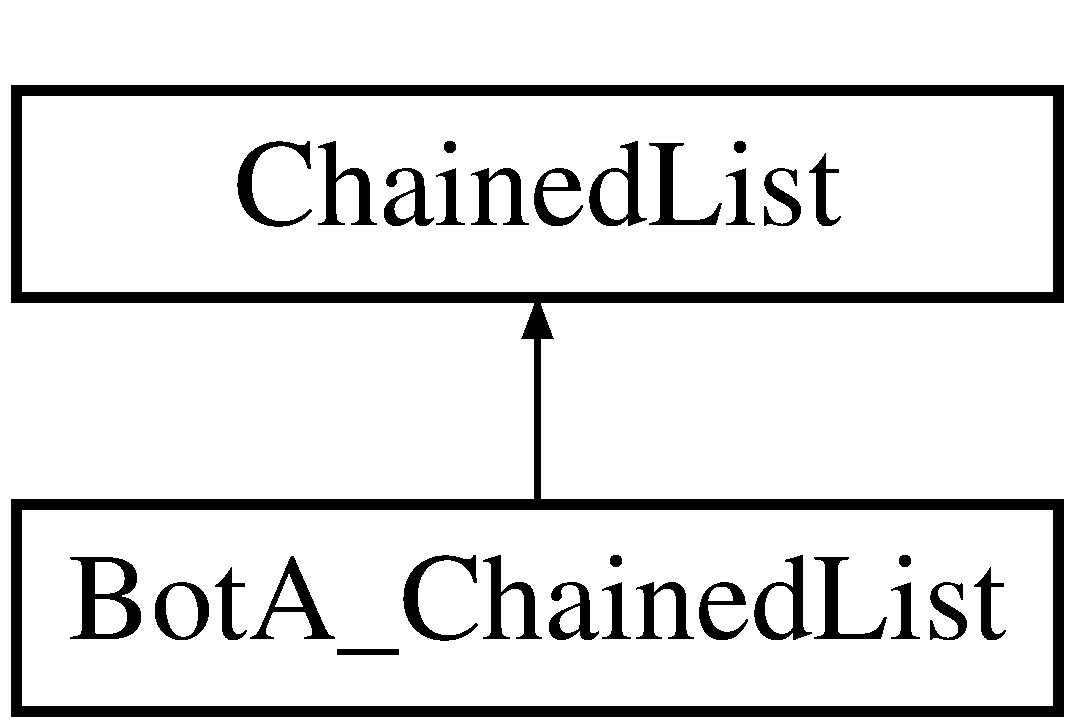
\includegraphics[height=2cm]{classBotA__ChainedList}
\end{center}
\end{figure}
\subsection*{Public Member Functions}
\begin{CompactItemize}
\item 
{\bf BotA\_\-ChainedList} ()
\end{CompactItemize}
\subsection*{Protected Member Functions}
\begin{CompactItemize}
\item 
virtual {\bf ListNode} $\ast$ {\bf createListNode} ({\bf TreeNode} $\ast$treeNode)
\end{CompactItemize}


\subsection{Detailed Description}
A specific version of \doxyref{ChainedList}{p.}{classChainedList} to use specific listNodes with heapStackCell values (only used with closeNodeList). 

\subsection{Constructor \& Destructor Documentation}
\index{BotA_ChainedList@{BotA\_\-ChainedList}!BotA_ChainedList@{BotA\_\-ChainedList}}
\index{BotA_ChainedList@{BotA\_\-ChainedList}!BotA_ChainedList@{BotA\_\-ChainedList}}
\subsubsection{\setlength{\rightskip}{0pt plus 5cm}BotA\_\-ChainedList::BotA\_\-ChainedList ()}\label{classBotA__ChainedList_80fa7bd09d33c568b6384d550a32334f}


Constructor of an empty chained list 

\subsection{Member Function Documentation}
\index{BotA_ChainedList@{BotA\_\-ChainedList}!createListNode@{createListNode}}
\index{createListNode@{createListNode}!BotA_ChainedList@{BotA\_\-ChainedList}}
\subsubsection{\setlength{\rightskip}{0pt plus 5cm}{\bf ListNode} $\ast$ BotA\_\-ChainedList::createListNode ({\bf TreeNode} $\ast$ {\em treeNode})\hspace{0.3cm}{\tt  [protected, virtual]}}\label{classBotA__ChainedList_0d0aa702abdd01801e3262ba55ed9315}


Destructor Create an \doxyref{ListNode}{p.}{classListNode} containing a treeNode \begin{Desc}
\item[Parameters:]
\begin{description}
\item[{\em treeNode}]\doxyref{TreeNode}{p.}{classTreeNode} to store in this \doxyref{ListNode}{p.}{classListNode} \end{description}
\end{Desc}
\begin{Desc}
\item[Returns:]New \doxyref{ListNode}{p.}{classListNode} filled with the treeNode argument \end{Desc}


Reimplemented from {\bf ChainedList} \doxyref{}{p.}{classChainedList_fa807d5bcc23ab479f10a3771fb22735}.

The documentation for this class was generated from the following files:\begin{CompactItemize}
\item 
include/Solver/BotA/BotA\_\-ChainedList.h\item 
src/Solver/BotA/BotA\_\-ChainedList.cpp\end{CompactItemize}

\section{BotA\_\-HashTable Class Reference}
\label{classBotA__HashTable}\index{BotA_HashTable@{BotA\_\-HashTable}}
A version of \doxyref{HashTable}{p.}{classHashTable} specific to closeNodeList in heap stack With it, we can get or change heapStackCell value of a specific node in the hashtable.  


{\tt \#include $<$BotA\_\-HashTable.h$>$}

Inheritance diagram for BotA\_\-HashTable::\begin{figure}[H]
\begin{center}
\leavevmode
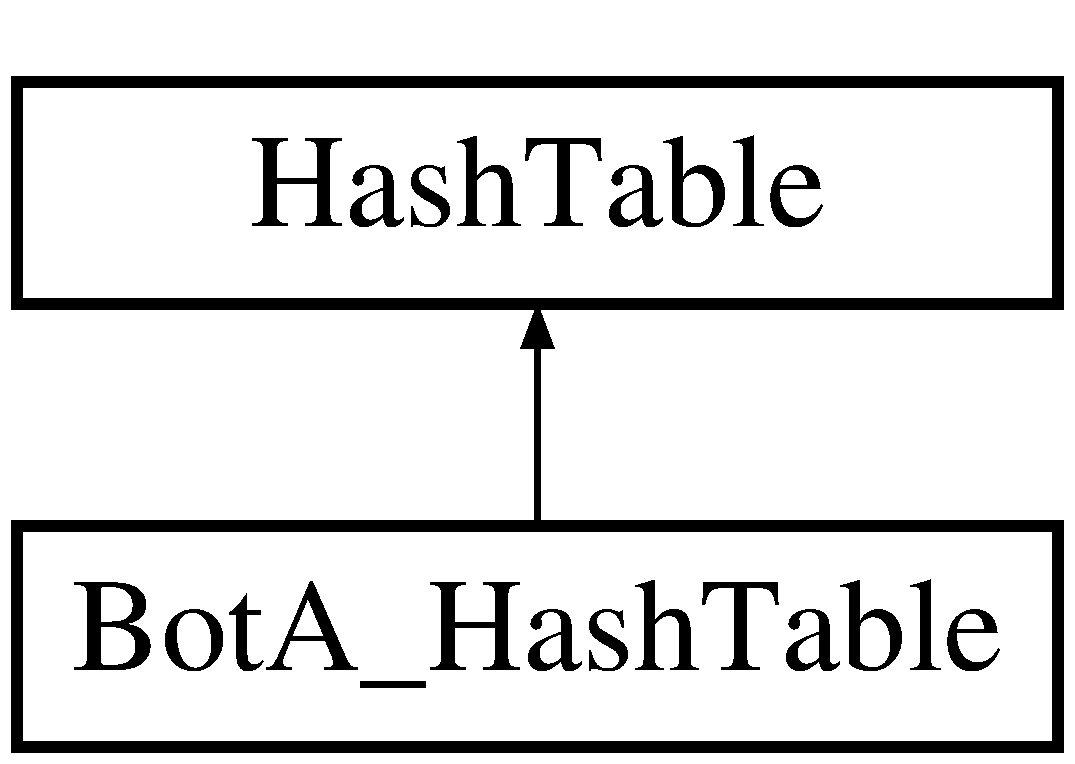
\includegraphics[height=2cm]{classBotA__HashTable}
\end{center}
\end{figure}
\subsection*{Public Member Functions}
\begin{CompactItemize}
\item 
{\bf BotA\_\-HashTable} (int {\bf length})
\item 
virtual bool {\bf isPresent} (const {\bf Node} $\ast$node) const 
\item 
int {\bf getHeapStackCell} (const {\bf Node} $\ast$node)
\item 
bool {\bf changeHeapStackCell} (const {\bf Node} $\ast$node, const int newHeapStackCell)
\end{CompactItemize}


\subsection{Detailed Description}
A version of \doxyref{HashTable}{p.}{classHashTable} specific to closeNodeList in heap stack With it, we can get or change heapStackCell value of a specific node in the hashtable. 

\subsection{Constructor \& Destructor Documentation}
\index{BotA_HashTable@{BotA\_\-HashTable}!BotA_HashTable@{BotA\_\-HashTable}}
\index{BotA_HashTable@{BotA\_\-HashTable}!BotA_HashTable@{BotA\_\-HashTable}}
\subsubsection{\setlength{\rightskip}{0pt plus 5cm}BotA\_\-HashTable::BotA\_\-HashTable (int {\em length})}\label{classBotA__HashTable_3e205cf3099dc18a978f6c17b6fdd276}


Constructor for new node \begin{Desc}
\item[Parameters:]
\begin{description}
\item[{\em treeNode}]treeNode to be stocked on this item \end{description}
\end{Desc}


\subsection{Member Function Documentation}
\index{BotA_HashTable@{BotA\_\-HashTable}!isPresent@{isPresent}}
\index{isPresent@{isPresent}!BotA_HashTable@{BotA\_\-HashTable}}
\subsubsection{\setlength{\rightskip}{0pt plus 5cm}bool BotA\_\-HashTable::isPresent (const {\bf Node} $\ast$ {\em node}) const\hspace{0.3cm}{\tt  [virtual]}}\label{classBotA__HashTable_e6005e8a8ed9551f640ecd325a8165f8}


Test if an \doxyref{Node}{p.}{classNode} is already present into the hashTable \begin{Desc}
\item[Parameters:]
\begin{description}
\item[{\em node}]\doxyref{Node}{p.}{classNode} we want to test \end{description}
\end{Desc}
\begin{Desc}
\item[Returns:]value of treenode (f(x)) is present, -1 if not \end{Desc}


Reimplemented from {\bf HashTable} \doxyref{}{p.}{classHashTable_1a1b16b0cfd69e0771cb55fe802229eb}.\index{BotA_HashTable@{BotA\_\-HashTable}!getHeapStackCell@{getHeapStackCell}}
\index{getHeapStackCell@{getHeapStackCell}!BotA_HashTable@{BotA\_\-HashTable}}
\subsubsection{\setlength{\rightskip}{0pt plus 5cm}int BotA\_\-HashTable::getHeapStackCell (const {\bf Node} $\ast$ {\em node})}\label{classBotA__HashTable_65499c783b7e18477c2091d4d690a955}


Get the heapStackCell value (cell number of node in the heapStack) from a node in the hashTable \begin{Desc}
\item[Parameters:]
\begin{description}
\item[{\em node}]node we want to get value \end{description}
\end{Desc}
\begin{Desc}
\item[Returns:]heapStackCell value of the node or -1 if value is not in the hashTable. \end{Desc}
\index{BotA_HashTable@{BotA\_\-HashTable}!changeHeapStackCell@{changeHeapStackCell}}
\index{changeHeapStackCell@{changeHeapStackCell}!BotA_HashTable@{BotA\_\-HashTable}}
\subsubsection{\setlength{\rightskip}{0pt plus 5cm}bool BotA\_\-HashTable::changeHeapStackCell (const {\bf Node} $\ast$ {\em node}, const int {\em newHeapStackCell})}\label{classBotA__HashTable_8c1cd848959157f7f9998c89a6f97780}


change the heapStackCell value (cell number of node in the heapStack) from a \doxyref{Node}{p.}{classNode} in the hashTable \begin{Desc}
\item[Parameters:]
\begin{description}
\item[{\em node}]node we want to change value \item[{\em newHeapStackCell}]new heap stack cell to assign to this node \end{description}
\end{Desc}
\begin{Desc}
\item[Returns:]true if value is changed, false if no node like this in the hashtable \end{Desc}


The documentation for this class was generated from the following files:\begin{CompactItemize}
\item 
include/Solver/BotA/BotA\_\-HashTable.h\item 
src/Solver/BotA/BotA\_\-HashTable.cpp\end{CompactItemize}

\section{BotA\_\-HeapStack Class Reference}
\label{classBotA__HeapStack}\index{BotA_HeapStack@{BotA\_\-HeapStack}}
A Heap Stack of TreeNodes. It can work like a chainedList to sort TreeNodes in order of cost. Smallest is always root treeNode of stack.  


{\tt \#include $<$BotA\_\-HeapStack.h$>$}

Inheritance diagram for BotA\_\-HeapStack::\begin{figure}[H]
\begin{center}
\leavevmode
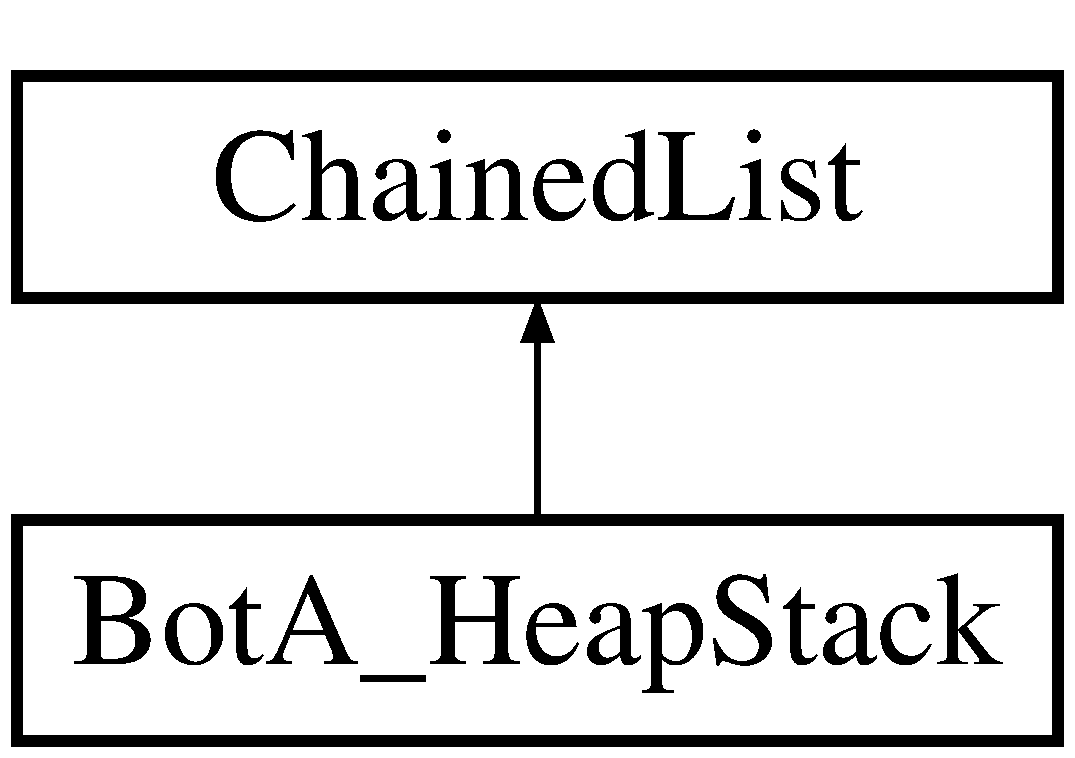
\includegraphics[height=2cm]{classBotA__HeapStack}
\end{center}
\end{figure}
\subsection*{Public Member Functions}
\begin{CompactItemize}
\item 
{\bf BotA\_\-HeapStack} ()
\item 
virtual {\bf $\sim$BotA\_\-HeapStack} ()
\item 
BotA\_\-TreeNode $\ast$$\ast$ {\bf getTreeNodeTab} (void) const 
\item 
int {\bf getTabLength} (void) const 
\item 
int {\bf getLength} (void) const 
\item 
void {\bf addItem} ({\bf TreeNode} $\ast$item)
\item 
virtual void {\bf deleteFirstItem} (void)
\item 
virtual {\bf ListNode} $\ast$ {\bf getFirstItem} (void) const 
\item 
virtual bool {\bf isSmaller} (int cell1, int cell2) const 
\item 
void {\bf repositionCell} (int cell)
\item 
virtual void {\bf addFirstItem} ({\bf TreeNode} $\ast$item)
\item 
virtual void {\bf addLastItem} ({\bf TreeNode} $\ast$item)
\item 
virtual void {\bf deleteLastItem} (void)
\end{CompactItemize}
\subsection*{Static Public Attributes}
\begin{CompactItemize}
\item 
static const int {\bf TAB\_\-MEMORY\_\-STEP} = 1000
\end{CompactItemize}
\subsection*{Protected Member Functions}
\begin{CompactItemize}
\item 
void {\bf minHeapify} (int cell)
\item 
int {\bf parent} (int cell)
\item 
int {\bf leftChild} (int cell)
\item 
int {\bf rightChild} (int cell)
\end{CompactItemize}
\subsection*{Protected Attributes}
\begin{CompactItemize}
\item 
BotA\_\-TreeNode $\ast$$\ast$ {\bf treeNodeTab}
\item 
int {\bf tabLength}
\end{CompactItemize}


\subsection{Detailed Description}
A Heap Stack of TreeNodes. It can work like a chainedList to sort TreeNodes in order of cost. Smallest is always root treeNode of stack. 

\subsection{Constructor \& Destructor Documentation}
\index{BotA_HeapStack@{BotA\_\-HeapStack}!BotA_HeapStack@{BotA\_\-HeapStack}}
\index{BotA_HeapStack@{BotA\_\-HeapStack}!BotA_HeapStack@{BotA\_\-HeapStack}}
\subsubsection{\setlength{\rightskip}{0pt plus 5cm}BotA\_\-HeapStack::BotA\_\-HeapStack ()}\label{classBotA__HeapStack_17543e44fa4f8a08750b100f29f49238}


Constructor of an empty chained list \index{BotA_HeapStack@{BotA\_\-HeapStack}!~BotA_HeapStack@{$\sim$BotA\_\-HeapStack}}
\index{~BotA_HeapStack@{$\sim$BotA\_\-HeapStack}!BotA_HeapStack@{BotA\_\-HeapStack}}
\subsubsection{\setlength{\rightskip}{0pt plus 5cm}BotA\_\-HeapStack::$\sim$BotA\_\-HeapStack ()\hspace{0.3cm}{\tt  [virtual]}}\label{classBotA__HeapStack_232e70d9e3caffb6bff404544d4d1c43}


Destructor 

\subsection{Member Function Documentation}
\index{BotA_HeapStack@{BotA\_\-HeapStack}!getTreeNodeTab@{getTreeNodeTab}}
\index{getTreeNodeTab@{getTreeNodeTab}!BotA_HeapStack@{BotA\_\-HeapStack}}
\subsubsection{\setlength{\rightskip}{0pt plus 5cm}BotA\_\-TreeNode$\ast$$\ast$ BotA\_\-HeapStack::getTreeNodeTab (void) const\hspace{0.3cm}{\tt  [inline]}}\label{classBotA__HeapStack_7739ac56fed46ceadd88ab11dc701a17}


table of treenodes \index{BotA_HeapStack@{BotA\_\-HeapStack}!getTabLength@{getTabLength}}
\index{getTabLength@{getTabLength}!BotA_HeapStack@{BotA\_\-HeapStack}}
\subsubsection{\setlength{\rightskip}{0pt plus 5cm}int BotA\_\-HeapStack::getTabLength (void) const\hspace{0.3cm}{\tt  [inline]}}\label{classBotA__HeapStack_44c289e02963fb3ebc0c02d433f5910c}


length of treenode table (not number of items but number of cells) \index{BotA_HeapStack@{BotA\_\-HeapStack}!getLength@{getLength}}
\index{getLength@{getLength}!BotA_HeapStack@{BotA\_\-HeapStack}}
\subsubsection{\setlength{\rightskip}{0pt plus 5cm}int BotA\_\-HeapStack::getLength (void) const\hspace{0.3cm}{\tt  [inline]}}\label{classBotA__HeapStack_6d9feab2ffbaad17131a7151b308d051}


number of items in table 

Reimplemented from {\bf ChainedList} \doxyref{}{p.}{classChainedList_8cf0661ee6c0e0f6259cd2e487fe94ce}.\index{BotA_HeapStack@{BotA\_\-HeapStack}!addItem@{addItem}}
\index{addItem@{addItem}!BotA_HeapStack@{BotA\_\-HeapStack}}
\subsubsection{\setlength{\rightskip}{0pt plus 5cm}void BotA\_\-HeapStack::addItem ({\bf TreeNode} $\ast$ {\em item})}\label{classBotA__HeapStack_9c84241a6a1d5a1a0dadea6c25b8ec68}


Add an item into the stack depending of the value of its cost. \begin{Desc}
\item[Parameters:]
\begin{description}
\item[{\em item}]\doxyref{TreeNode}{p.}{classTreeNode} to add to the stack \end{description}
\end{Desc}
\index{BotA_HeapStack@{BotA\_\-HeapStack}!deleteFirstItem@{deleteFirstItem}}
\index{deleteFirstItem@{deleteFirstItem}!BotA_HeapStack@{BotA\_\-HeapStack}}
\subsubsection{\setlength{\rightskip}{0pt plus 5cm}void BotA\_\-HeapStack::deleteFirstItem (void)\hspace{0.3cm}{\tt  [virtual]}}\label{classBotA__HeapStack_798de6d8fe135f04a2d76a36eff147cd}


Delete first item of the stack and 

Reimplemented from {\bf ChainedList} \doxyref{}{p.}{classChainedList_01dc3f81d3a912ec2455734cdf2d1e46}.\index{BotA_HeapStack@{BotA\_\-HeapStack}!getFirstItem@{getFirstItem}}
\index{getFirstItem@{getFirstItem}!BotA_HeapStack@{BotA\_\-HeapStack}}
\subsubsection{\setlength{\rightskip}{0pt plus 5cm}{\bf ListNode} $\ast$ BotA\_\-HeapStack::getFirstItem (void) const\hspace{0.3cm}{\tt  [virtual]}}\label{classBotA__HeapStack_ebe93c0a849f73fa773e24ffc0aa16e8}


root item of the stack in a \doxyref{ListNode}{p.}{classListNode} for compatibilty with solver 

Reimplemented from {\bf ChainedList} \doxyref{}{p.}{classChainedList_fb20aaef36ab32d23a35bb0c909715b2}.\index{BotA_HeapStack@{BotA\_\-HeapStack}!isSmaller@{isSmaller}}
\index{isSmaller@{isSmaller}!BotA_HeapStack@{BotA\_\-HeapStack}}
\subsubsection{\setlength{\rightskip}{0pt plus 5cm}bool BotA\_\-HeapStack::isSmaller (int {\em cell1}, int {\em cell2}) const\hspace{0.3cm}{\tt  [virtual]}}\label{classBotA__HeapStack_2b59d857afbee3c2eedd6bb516e12942}


Test cost of 2 treenodes position in treeNodeTab \begin{Desc}
\item[Parameters:]
\begin{description}
\item[{\em cell1}]first cell position to test \item[{\em cell2}]second cell position to test \end{description}
\end{Desc}
\begin{Desc}
\item[Returns:]true if cost of treeNodeTab[cell1] is smaller than cost of treeNodeTab[cell2] \end{Desc}
\index{BotA_HeapStack@{BotA\_\-HeapStack}!repositionCell@{repositionCell}}
\index{repositionCell@{repositionCell}!BotA_HeapStack@{BotA\_\-HeapStack}}
\subsubsection{\setlength{\rightskip}{0pt plus 5cm}void BotA\_\-HeapStack::repositionCell (int {\em cell})}\label{classBotA__HeapStack_95f898c1e623d6a9456ea51bca4d7e10}


Re-position a cell of the tab (node in the heap stack) at this right position depending of its new lesser value than before \begin{Desc}
\item[Parameters:]
\begin{description}
\item[{\em cell}]cell we want to re-position depending of its new lesser value \end{description}
\end{Desc}
\index{BotA_HeapStack@{BotA\_\-HeapStack}!addFirstItem@{addFirstItem}}
\index{addFirstItem@{addFirstItem}!BotA_HeapStack@{BotA\_\-HeapStack}}
\subsubsection{\setlength{\rightskip}{0pt plus 5cm}void BotA\_\-HeapStack::addFirstItem ({\bf TreeNode} $\ast$ {\em item})\hspace{0.3cm}{\tt  [virtual]}}\label{classBotA__HeapStack_7ab05ef7a0237229c5973e95cfcefc1c}


Unused functions with Heap Stack search 

Reimplemented from {\bf ChainedList} \doxyref{}{p.}{classChainedList_52ad982ab220ad0eea5513180f434db2}.\index{BotA_HeapStack@{BotA\_\-HeapStack}!addLastItem@{addLastItem}}
\index{addLastItem@{addLastItem}!BotA_HeapStack@{BotA\_\-HeapStack}}
\subsubsection{\setlength{\rightskip}{0pt plus 5cm}void BotA\_\-HeapStack::addLastItem ({\bf TreeNode} $\ast$ {\em item})\hspace{0.3cm}{\tt  [virtual]}}\label{classBotA__HeapStack_aef3826b63645c27d10e7f673211fe94}


Add an item to the end of the chainedlist \begin{Desc}
\item[Parameters:]
\begin{description}
\item[{\em item}]Item to add \end{description}
\end{Desc}


Reimplemented from {\bf ChainedList} \doxyref{}{p.}{classChainedList_92aa990058d417146bc43beed16c90f6}.\index{BotA_HeapStack@{BotA\_\-HeapStack}!deleteLastItem@{deleteLastItem}}
\index{deleteLastItem@{deleteLastItem}!BotA_HeapStack@{BotA\_\-HeapStack}}
\subsubsection{\setlength{\rightskip}{0pt plus 5cm}void BotA\_\-HeapStack::deleteLastItem (void)\hspace{0.3cm}{\tt  [virtual]}}\label{classBotA__HeapStack_3d787006c437d954881f2c3833b6190b}


Delete last item of the list 

Reimplemented from {\bf ChainedList} \doxyref{}{p.}{classChainedList_de017c8ad7cbfc4d347473bf303b1da2}.\index{BotA_HeapStack@{BotA\_\-HeapStack}!minHeapify@{minHeapify}}
\index{minHeapify@{minHeapify}!BotA_HeapStack@{BotA\_\-HeapStack}}
\subsubsection{\setlength{\rightskip}{0pt plus 5cm}void BotA\_\-HeapStack::minHeapify (int {\em cell})\hspace{0.3cm}{\tt  [protected]}}\label{classBotA__HeapStack_71026f74850281d6435dc071448057af}


Put a cell of the tab (node in the heap Stack) at its right position depending of its value (move down the tree if necessary but never up) \begin{Desc}
\item[Parameters:]
\begin{description}
\item[{\em cell}]cell we want to move if necessary \end{description}
\end{Desc}
\index{BotA_HeapStack@{BotA\_\-HeapStack}!parent@{parent}}
\index{parent@{parent}!BotA_HeapStack@{BotA\_\-HeapStack}}
\subsubsection{\setlength{\rightskip}{0pt plus 5cm}int BotA\_\-HeapStack::parent (int {\em cell})\hspace{0.3cm}{\tt  [inline, protected]}}\label{classBotA__HeapStack_3920a89f0d98aeadfcf2f540f2148838}


Get parent node of a cell of the tab \begin{Desc}
\item[Parameters:]
\begin{description}
\item[{\em cell}]cell we want to find parent \end{description}
\end{Desc}
\begin{Desc}
\item[Returns:]num of parent cell in tab \end{Desc}
\index{BotA_HeapStack@{BotA\_\-HeapStack}!leftChild@{leftChild}}
\index{leftChild@{leftChild}!BotA_HeapStack@{BotA\_\-HeapStack}}
\subsubsection{\setlength{\rightskip}{0pt plus 5cm}int BotA\_\-HeapStack::leftChild (int {\em cell})\hspace{0.3cm}{\tt  [inline, protected]}}\label{classBotA__HeapStack_869d79be31cdb2f69b77b97af6d88482}


Get left child node of a cell of the tab \begin{Desc}
\item[Parameters:]
\begin{description}
\item[{\em cell}]cell we want to find left child node \end{description}
\end{Desc}
\begin{Desc}
\item[Returns:]num of left child cell in tab \end{Desc}
\index{BotA_HeapStack@{BotA\_\-HeapStack}!rightChild@{rightChild}}
\index{rightChild@{rightChild}!BotA_HeapStack@{BotA\_\-HeapStack}}
\subsubsection{\setlength{\rightskip}{0pt plus 5cm}int BotA\_\-HeapStack::rightChild (int {\em cell})\hspace{0.3cm}{\tt  [inline, protected]}}\label{classBotA__HeapStack_cb75b4e244ac2c48253b0c53885477b0}


Get right child node of a cell of the tab \begin{Desc}
\item[Parameters:]
\begin{description}
\item[{\em cell}]cell we want to find right child node \end{description}
\end{Desc}
\begin{Desc}
\item[Returns:]num of right child cell in tab \end{Desc}


\subsection{Member Data Documentation}
\index{BotA_HeapStack@{BotA\_\-HeapStack}!treeNodeTab@{treeNodeTab}}
\index{treeNodeTab@{treeNodeTab}!BotA_HeapStack@{BotA\_\-HeapStack}}
\subsubsection{\setlength{\rightskip}{0pt plus 5cm}BotA\_\-TreeNode$\ast$$\ast$ {\bf BotA\_\-HeapStack::treeNodeTab}\hspace{0.3cm}{\tt  [protected]}}\label{classBotA__HeapStack_1fe52f81088565146a0dde5e5b949d47}


Tab of (closed) treenodes sorted by heap stack (see implementation of heap stack to know why we use a tab and not a tree). \index{BotA_HeapStack@{BotA\_\-HeapStack}!tabLength@{tabLength}}
\index{tabLength@{tabLength}!BotA_HeapStack@{BotA\_\-HeapStack}}
\subsubsection{\setlength{\rightskip}{0pt plus 5cm}int {\bf BotA\_\-HeapStack::tabLength}\hspace{0.3cm}{\tt  [protected]}}\label{classBotA__HeapStack_d43c3f89411288466a3eda349689b028}


Length of the treeNode tab \index{BotA_HeapStack@{BotA\_\-HeapStack}!TAB_MEMORY_STEP@{TAB\_\-MEMORY\_\-STEP}}
\index{TAB_MEMORY_STEP@{TAB\_\-MEMORY\_\-STEP}!BotA_HeapStack@{BotA\_\-HeapStack}}
\subsubsection{\setlength{\rightskip}{0pt plus 5cm}const int {\bf BotA\_\-HeapStack::TAB\_\-MEMORY\_\-STEP} = 1000\hspace{0.3cm}{\tt  [static]}}\label{classBotA__HeapStack_8f2f4081317b23e52b0be851dba07965}


alloc and dealloc step of tab 

The documentation for this class was generated from the following files:\begin{CompactItemize}
\item 
include/Solver/BotA/BotA\_\-HeapStack.h\item 
src/Solver/BotA/BotA\_\-HeapStack.cpp\end{CompactItemize}

\section{BotA\_\-ListNode Class Reference}
\label{classBotA__ListNode}\index{BotA_ListNode@{BotA\_\-ListNode}}
A version of \doxyref{ListNode}{p.}{classListNode} with \char`\"{}f\char`\"{} and \char`\"{}g\char`\"{} getters where f(x)=g(x)+h(x). It's used to make the A$\ast$ solver.  


{\tt \#include $<$BotA\_\-ListNode.h$>$}

Inheritance diagram for BotA\_\-ListNode::\begin{figure}[H]
\begin{center}
\leavevmode
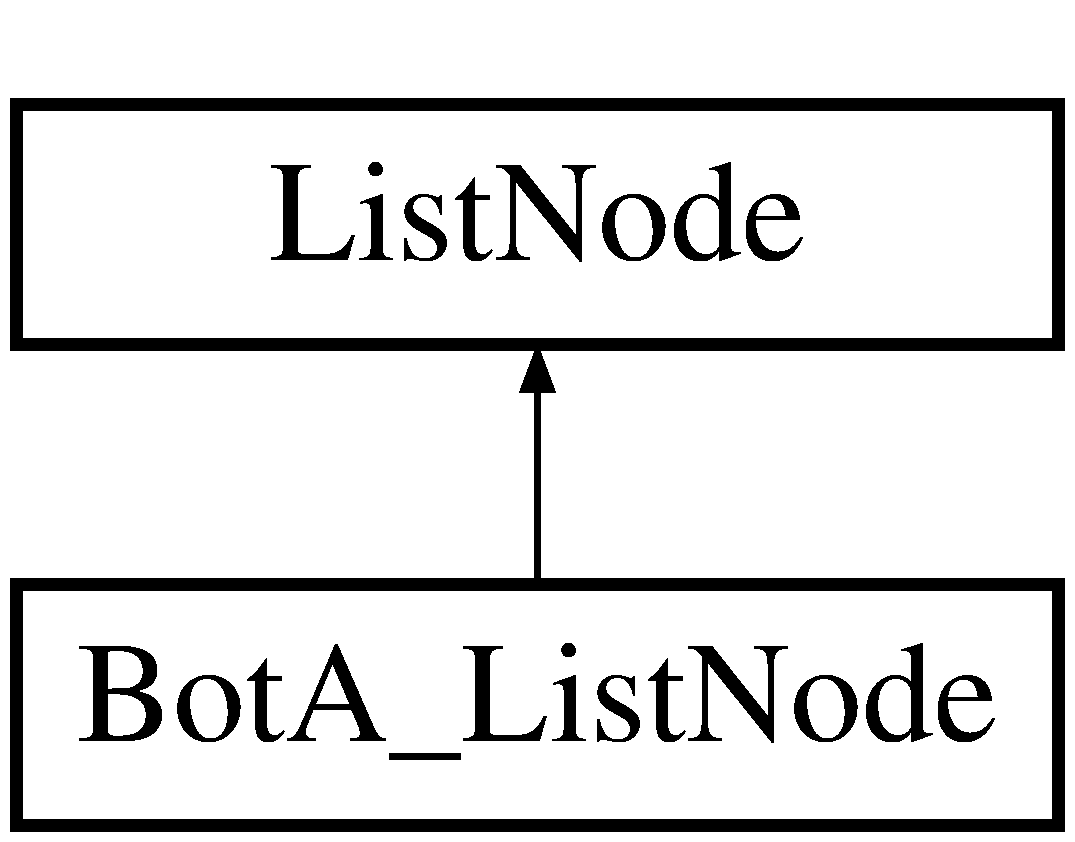
\includegraphics[height=2cm]{classBotA__ListNode}
\end{center}
\end{figure}
\subsection*{Public Member Functions}
\begin{CompactItemize}
\item 
{\bf BotA\_\-ListNode} ({\bf TreeNode} $\ast${\bf treeNode})
\item 
int {\bf getF} (void) const 
\item 
int {\bf getG} (void) const 
\item 
int {\bf getH} (void) const 
\end{CompactItemize}


\subsection{Detailed Description}
A version of \doxyref{ListNode}{p.}{classListNode} with \char`\"{}f\char`\"{} and \char`\"{}g\char`\"{} getters where f(x)=g(x)+h(x). It's used to make the A$\ast$ solver. 

\subsection{Constructor \& Destructor Documentation}
\index{BotA_ListNode@{BotA\_\-ListNode}!BotA_ListNode@{BotA\_\-ListNode}}
\index{BotA_ListNode@{BotA\_\-ListNode}!BotA_ListNode@{BotA\_\-ListNode}}
\subsubsection{\setlength{\rightskip}{0pt plus 5cm}BotA\_\-ListNode::BotA\_\-ListNode ({\bf TreeNode} $\ast$ {\em treeNode})}\label{classBotA__ListNode_fd79ea26994bac4e30ddcde3f21abf8d}


Constructor for empty node \begin{Desc}
\item[Parameters:]
\begin{description}
\item[{\em treeNode}]treeNode to be stocked on this item \end{description}
\end{Desc}


\subsection{Member Function Documentation}
\index{BotA_ListNode@{BotA\_\-ListNode}!getF@{getF}}
\index{getF@{getF}!BotA_ListNode@{BotA\_\-ListNode}}
\subsubsection{\setlength{\rightskip}{0pt plus 5cm}int BotA\_\-ListNode::getF (void) const\hspace{0.3cm}{\tt  [inline]}}\label{classBotA__ListNode_cee4207413e0d073568133b8711c2bf3}


f(x) value \index{BotA_ListNode@{BotA\_\-ListNode}!getG@{getG}}
\index{getG@{getG}!BotA_ListNode@{BotA\_\-ListNode}}
\subsubsection{\setlength{\rightskip}{0pt plus 5cm}int BotA\_\-ListNode::getG (void) const\hspace{0.3cm}{\tt  [inline]}}\label{classBotA__ListNode_ad2ef2eb526cab5d6e3dc06155bf2d07}


g(x) value \index{BotA_ListNode@{BotA\_\-ListNode}!getH@{getH}}
\index{getH@{getH}!BotA_ListNode@{BotA\_\-ListNode}}
\subsubsection{\setlength{\rightskip}{0pt plus 5cm}int BotA\_\-ListNode::getH (void) const\hspace{0.3cm}{\tt  [inline]}}\label{classBotA__ListNode_16501a9982c49077d9fcd7bbf7a200e7}


h(x) value 

The documentation for this class was generated from the following files:\begin{CompactItemize}
\item 
include/Solver/BotA/BotA\_\-ListNode.h\item 
src/Solver/BotA/BotA\_\-ListNode.cpp\end{CompactItemize}

\section{BotA\_\-ListNode2 Class Reference}
\label{classBotA__ListNode2}\index{BotA_ListNode2@{BotA\_\-ListNode2}}
A version of \doxyref{ListNode}{p.}{classListNode} with \char`\"{}f\char`\"{} and \char`\"{}g\char`\"{} getters where f(x)=g(x)+h(x). It's used to make the A$\ast$ solver WARNING : this second version of \doxyref{ListNode}{p.}{classListNode} is dedicated to close hashtable and use one more variable : \char`\"{}heapStackCell\char`\"{}. heapStackCell is the number of cell treeNode of this Listnode is currently in.  


{\tt \#include $<$BotA\_\-ListNode2.h$>$}

Inheritance diagram for BotA\_\-ListNode2::\begin{figure}[H]
\begin{center}
\leavevmode
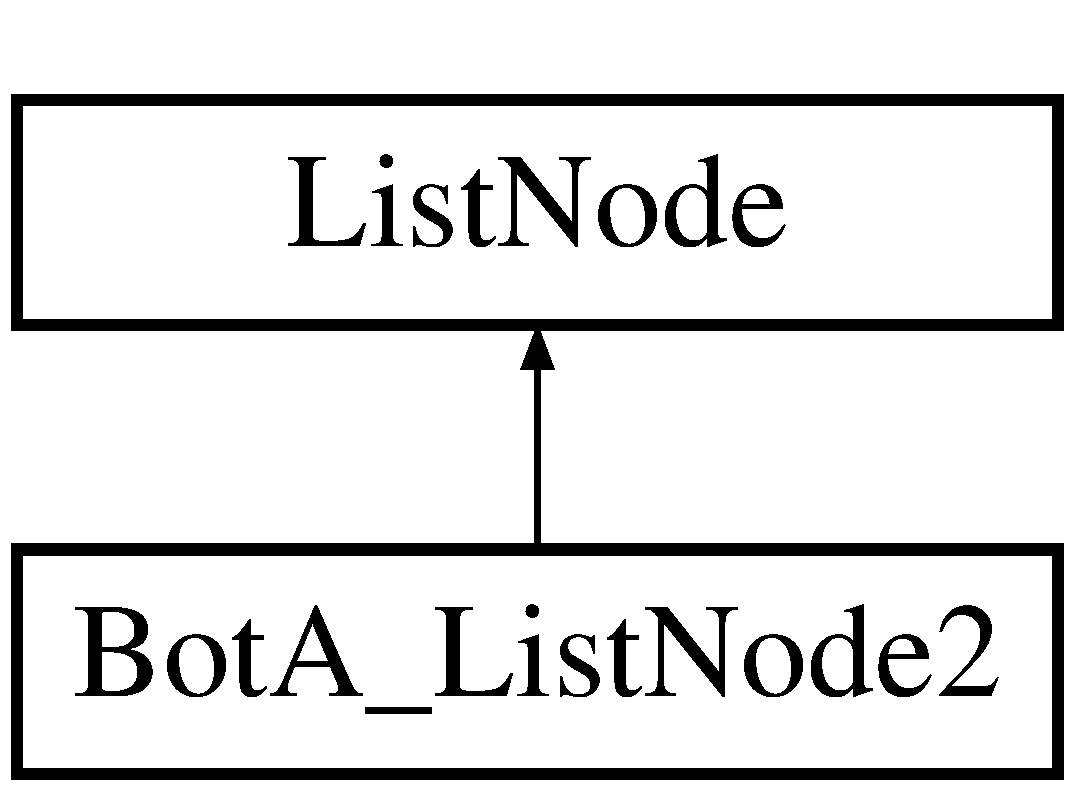
\includegraphics[height=2cm]{classBotA__ListNode2}
\end{center}
\end{figure}
\subsection*{Public Member Functions}
\begin{CompactItemize}
\item 
{\bf BotA\_\-ListNode2} ({\bf TreeNode} $\ast${\bf treeNode})
\item 
{\bf BotA\_\-ListNode2} ({\bf TreeNode} $\ast${\bf treeNode}, int {\bf heapStackCell})
\item 
int {\bf getF} (void) const 
\item 
int {\bf getG} (void) const 
\item 
int {\bf getH} (void) const 
\item 
int {\bf getHeapStackCell} (void) const 
\item 
void {\bf setHeapStackCell} (int {\bf heapStackCell})
\end{CompactItemize}
\subsection*{Protected Attributes}
\begin{CompactItemize}
\item 
int {\bf heapStackCell}
\end{CompactItemize}


\subsection{Detailed Description}
A version of \doxyref{ListNode}{p.}{classListNode} with \char`\"{}f\char`\"{} and \char`\"{}g\char`\"{} getters where f(x)=g(x)+h(x). It's used to make the A$\ast$ solver WARNING : this second version of \doxyref{ListNode}{p.}{classListNode} is dedicated to close hashtable and use one more variable : \char`\"{}heapStackCell\char`\"{}. heapStackCell is the number of cell treeNode of this Listnode is currently in. 

\subsection{Constructor \& Destructor Documentation}
\index{BotA_ListNode2@{BotA\_\-ListNode2}!BotA_ListNode2@{BotA\_\-ListNode2}}
\index{BotA_ListNode2@{BotA\_\-ListNode2}!BotA_ListNode2@{BotA\_\-ListNode2}}
\subsubsection{\setlength{\rightskip}{0pt plus 5cm}BotA\_\-ListNode2::BotA\_\-ListNode2 ({\bf TreeNode} $\ast$ {\em treeNode})}\label{classBotA__ListNode2_744f419bf670aa28bd55e51908984175}


Constructor for new node \begin{Desc}
\item[Parameters:]
\begin{description}
\item[{\em treeNode}]treeNode to be stocked on this item \end{description}
\end{Desc}
\index{BotA_ListNode2@{BotA\_\-ListNode2}!BotA_ListNode2@{BotA\_\-ListNode2}}
\index{BotA_ListNode2@{BotA\_\-ListNode2}!BotA_ListNode2@{BotA\_\-ListNode2}}
\subsubsection{\setlength{\rightskip}{0pt plus 5cm}BotA\_\-ListNode2::BotA\_\-ListNode2 ({\bf TreeNode} $\ast$ {\em treeNode}, int {\em heapStackCell})}\label{classBotA__ListNode2_4ad9b6c38517f87bff4a47f4da0f518b}


Constructor for new node \begin{Desc}
\item[Parameters:]
\begin{description}
\item[{\em treeNode}]treeNode to be stocked on this item \item[{\em heapStackCell}]Number of cell this treeNode is on heap stack \end{description}
\end{Desc}


\subsection{Member Function Documentation}
\index{BotA_ListNode2@{BotA\_\-ListNode2}!getF@{getF}}
\index{getF@{getF}!BotA_ListNode2@{BotA\_\-ListNode2}}
\subsubsection{\setlength{\rightskip}{0pt plus 5cm}int BotA\_\-ListNode2::getF (void) const\hspace{0.3cm}{\tt  [inline]}}\label{classBotA__ListNode2_47be9d3348d65e5398d0cd21a2a5bf7e}


f(x) value \index{BotA_ListNode2@{BotA\_\-ListNode2}!getG@{getG}}
\index{getG@{getG}!BotA_ListNode2@{BotA\_\-ListNode2}}
\subsubsection{\setlength{\rightskip}{0pt plus 5cm}int BotA\_\-ListNode2::getG (void) const\hspace{0.3cm}{\tt  [inline]}}\label{classBotA__ListNode2_6954ebea0a96ff87724081f061cbcc8c}


g(x) value \index{BotA_ListNode2@{BotA\_\-ListNode2}!getH@{getH}}
\index{getH@{getH}!BotA_ListNode2@{BotA\_\-ListNode2}}
\subsubsection{\setlength{\rightskip}{0pt plus 5cm}int BotA\_\-ListNode2::getH (void) const\hspace{0.3cm}{\tt  [inline]}}\label{classBotA__ListNode2_e36ff05e3724c201c1a78d69f5f0f50d}


h(x) value \index{BotA_ListNode2@{BotA\_\-ListNode2}!getHeapStackCell@{getHeapStackCell}}
\index{getHeapStackCell@{getHeapStackCell}!BotA_ListNode2@{BotA\_\-ListNode2}}
\subsubsection{\setlength{\rightskip}{0pt plus 5cm}int BotA\_\-ListNode2::getHeapStackCell (void) const\hspace{0.3cm}{\tt  [inline]}}\label{classBotA__ListNode2_91b67f8b4eeb63cf63786b10e9f7c45b}


heapStackCell value \index{BotA_ListNode2@{BotA\_\-ListNode2}!setHeapStackCell@{setHeapStackCell}}
\index{setHeapStackCell@{setHeapStackCell}!BotA_ListNode2@{BotA\_\-ListNode2}}
\subsubsection{\setlength{\rightskip}{0pt plus 5cm}void BotA\_\-ListNode2::setHeapStackCell (int {\em heapStackCell})\hspace{0.3cm}{\tt  [inline]}}\label{classBotA__ListNode2_64d192ed333dfe207bec84c28e8b6bf3}


Set heapStackCell value 

\subsection{Member Data Documentation}
\index{BotA_ListNode2@{BotA\_\-ListNode2}!heapStackCell@{heapStackCell}}
\index{heapStackCell@{heapStackCell}!BotA_ListNode2@{BotA\_\-ListNode2}}
\subsubsection{\setlength{\rightskip}{0pt plus 5cm}int {\bf BotA\_\-ListNode2::heapStackCell}\hspace{0.3cm}{\tt  [protected]}}\label{classBotA__ListNode2_7d599584e366ba21c4afb894acabec62}


Number of cell treeNode is currently in 

The documentation for this class was generated from the following files:\begin{CompactItemize}
\item 
include/Solver/BotA/BotA\_\-ListNode2.h\item 
src/Solver/BotA/BotA\_\-ListNode2.cpp\end{CompactItemize}

\section{BotBestMovesS Class Reference}
\label{classBotBestMovesS}\index{BotBestMovesS@{BotBestMovesS}}
A$\ast$ algorithm based on moves number of the pusher. Nodes with less moves are explored first. WARNING : this algorithm doesn't return best moves solution of this level but only a good solution. This is because a state representation of the level doesn't keep exact pusher position but only a pusher zone. This solver will work efficiently (but with a lot of extra work) only if we make level representation with boxes position (zone) and exact pusher position (integer).  


{\tt \#include $<$BotBestMovesS.h$>$}

Inheritance diagram for BotBestMovesS::\begin{figure}[H]
\begin{center}
\leavevmode
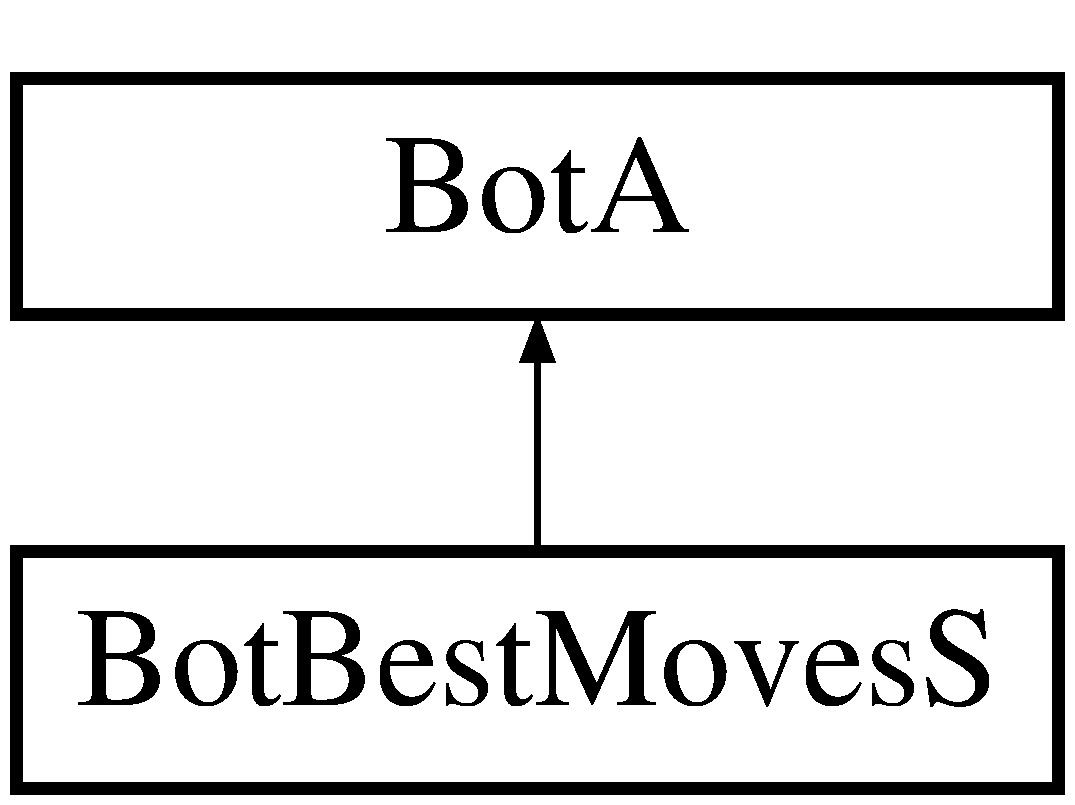
\includegraphics[height=2cm]{classBotBestMovesS}
\end{center}
\end{figure}
\subsection*{Public Member Functions}
\begin{CompactItemize}
\item 
virtual const char $\ast$ {\bf SOLVER\_\-NAME} ()
\item 
{\bf BotBestMovesS} (Base $\ast$base, {\bf Level} $\ast$level, int maxNodeNumber, int maxRamSize, int openTableSize, int closeTableSize, int {\bf costLimit}, int deadlockedBoxesSearch=2)
\item 
virtual int {\bf f} ({\bf TreeNode} $\ast$treeNode) const 
\item 
virtual int {\bf h} ({\bf TreeNode} $\ast$treeNode) const 
\end{CompactItemize}


\subsection{Detailed Description}
A$\ast$ algorithm based on moves number of the pusher. Nodes with less moves are explored first. WARNING : this algorithm doesn't return best moves solution of this level but only a good solution. This is because a state representation of the level doesn't keep exact pusher position but only a pusher zone. This solver will work efficiently (but with a lot of extra work) only if we make level representation with boxes position (zone) and exact pusher position (integer). 

\subsection{Constructor \& Destructor Documentation}
\index{BotBestMovesS@{BotBestMovesS}!BotBestMovesS@{BotBestMovesS}}
\index{BotBestMovesS@{BotBestMovesS}!BotBestMovesS@{BotBestMovesS}}
\subsubsection{\setlength{\rightskip}{0pt plus 5cm}BotBestMovesS::BotBestMovesS (Base $\ast$ {\em base}, {\bf Level} $\ast$ {\em level}, int {\em maxNodeNumber}, int {\em maxRamSize}, int {\em openTableSize}, int {\em closeTableSize}, int {\em costLimit}, int {\em deadlockedBoxesSearch} = {\tt 2})}\label{classBotBestMovesS_4f949103618847e78611d02647293072}


Constructor for a solver of a level \begin{Desc}
\item[Parameters:]
\begin{description}
\item[{\em base}]main class of the game \item[{\em level}]\doxyref{Level}{p.}{classLevel} to be used \item[{\em maxNodeNumber}]Limit number of nodes to explore \item[{\em maxRamSize}]Limit max ram size to allocate \item[{\em openTableSize}]size of Open Table to allocate (hashtable) \item[{\em closeTableSize}]size of Close Table to allocate (hashtable) \item[{\em limit}]of accepted f(x). if costLimit = -1, costLimit = +infinity \item[{\em deadlockedBoxesSearch}]number of boxes to use when testing every possible positions of deadlock \end{description}
\end{Desc}


\subsection{Member Function Documentation}
\index{BotBestMovesS@{BotBestMovesS}!SOLVER_NAME@{SOLVER\_\-NAME}}
\index{SOLVER_NAME@{SOLVER\_\-NAME}!BotBestMovesS@{BotBestMovesS}}
\subsubsection{\setlength{\rightskip}{0pt plus 5cm}virtual const char$\ast$ BotBestMovesS::SOLVER\_\-NAME ()\hspace{0.3cm}{\tt  [inline, virtual]}}\label{classBotBestMovesS_c29b9292fd9d234d1d4e7c8ef4e36720}


Name of this solver 

Implements {\bf BotA} \doxyref{}{p.}{classBotA_ab85547e677baf43658369ab19a461c4}.\index{BotBestMovesS@{BotBestMovesS}!f@{f}}
\index{f@{f}!BotBestMovesS@{BotBestMovesS}}
\subsubsection{\setlength{\rightskip}{0pt plus 5cm}int BotBestMovesS::f ({\bf TreeNode} $\ast$ {\em treeNode}) const\hspace{0.3cm}{\tt  [virtual]}}\label{classBotBestMovesS_e30409d7af027a14505718843653893c}


Cost function to evaluate the cost of a treenode with its position in the tree (parent of treenode must be assigned before calling this function) this cost function will compute number of moves from the start until this node. So we can search min moves number first WARNING : not finished yet, to be really efficient, h(x) must be definied \index{BotBestMovesS@{BotBestMovesS}!h@{h}}
\index{h@{h}!BotBestMovesS@{BotBestMovesS}}
\subsubsection{\setlength{\rightskip}{0pt plus 5cm}int BotBestMovesS::h ({\bf TreeNode} $\ast$ {\em treeNode}) const\hspace{0.3cm}{\tt  [virtual]}}\label{classBotBestMovesS_737fff641aa19f3d89cf98cf87c6ba76}


Cost function to evaluate the cost of admissibly estimated distance to a goal treenode from this treenode (parent of treenode must be assigned before calling this function) 

Implements {\bf BotA} \doxyref{}{p.}{classBotA_c9d54cca141a1f1638a3482a616e9403}.

The documentation for this class was generated from the following files:\begin{CompactItemize}
\item 
include/Solver/BotBestMovesS/BotBestMovesS.h\item 
src/Solver/BotBestMovesS/BotBestMovesS.cpp\end{CompactItemize}

\section{BotBestPushesS\_\-Penalties Class Reference}
\label{classBotBestPushesS__Penalties}\index{BotBestPushesS_Penalties@{BotBestPushesS\_\-Penalties}}
Management of cost penalties. Try to detect every sub-states that causes a penalty to the initial cost.  


{\tt \#include $<$BotBestPushesS\_\-Penalties.h$>$}

\subsection*{Public Member Functions}
\begin{CompactItemize}
\item 
{\bf BotBestPushesS\_\-Penalties} (Solver $\ast${\bf solver})
\item 
{\bf $\sim$BotBestPushesS\_\-Penalties} ()
\item 
Solver $\ast$ {\bf getSolver} (void) const 
\item 
{\bf Node} $\ast$$\ast$$\ast$ {\bf getPenaltiesNodeList} (void) const 
\item 
{\bf Level} $\ast$ {\bf getEmptyLevel} (void) const 
\item 
int {\bf getPenaltyOfTreeNode} ({\bf TreeNode} $\ast$treenode) const 
\item 
bool {\bf penaltiesListTest} (int $\ast$tab, int tabLength, int $\ast$nodeLimit=NULL, int pusherLevelPos=-1)
\end{CompactItemize}
\subsection*{Protected Member Functions}
\begin{CompactItemize}
\item 
void {\bf addToPNodes} ({\bf Node} $\ast$newPenalizedNode, int penalty, int numOfBoxes)
\item 
void {\bf orderList} (int index) const 
\item 
void {\bf initPenaltiesList} (int numberOfBoxes)
\item 
void {\bf createPenaltiesList} (int numberOfBoxes)
\item 
void {\bf savePenaltiesList} ()
\item 
void {\bf loadPenaltiesList} (char $\ast$fileName, int numberOfBoxes)
\item 
void {\bf increasePenaltiesListTest} (int positions, int $\ast$$\ast$tab, int $\ast$tabLength)
\item 
bool {\bf lastPenaltiesListTest} (int positions, int $\ast$tab, int tabLength)
\item 
int {\bf validNode} ({\bf Node} $\ast$node, int numOfBoxes, int prereq, int penaltyDown, int penaltyUp, bool quickValid=false, int maxNodes=INT\_\-MAX)
\item 
bool {\bf isUselessPenalty} ({\bf Level} $\ast$l)
\item 
bool {\bf ramLimitReached} (char $\ast$message) const 
\item 
bool {\bf notResolved} (char $\ast$message) const 
\end{CompactItemize}
\subsection*{Protected Attributes}
\begin{CompactItemize}
\item 
Base $\ast$ {\bf base}
\item 
Solver $\ast$ {\bf solver}
\item 
{\bf Node} $\ast$$\ast$$\ast$ {\bf pNodes}
\item 
int $\ast$$\ast$ {\bf pValues}
\item 
int {\bf pLength}
\item 
int $\ast$ {\bf pListLengths}
\item 
int $\ast$ {\bf penaltiesTestTab}
\item 
int {\bf penaltiesTestTabLength}
\item 
{\bf Level} $\ast$ {\bf emptyLevel}
\item 
const {\bf Level} $\ast$ {\bf level}
\item 
const {\bf Zone} $\ast$ {\bf goalZone}
\item 
const int $\ast$ {\bf zoneToLevelPos}
\item 
const int {\bf zoneToLevelPosLength}
\item 
const int $\ast$ {\bf levelToZonePos}
\end{CompactItemize}


\subsection{Detailed Description}
Management of cost penalties. Try to detect every sub-states that causes a penalty to the initial cost. 

\subsection{Constructor \& Destructor Documentation}
\index{BotBestPushesS_Penalties@{BotBestPushesS\_\-Penalties}!BotBestPushesS_Penalties@{BotBestPushesS\_\-Penalties}}
\index{BotBestPushesS_Penalties@{BotBestPushesS\_\-Penalties}!BotBestPushesS_Penalties@{BotBestPushesS\_\-Penalties}}
\subsubsection{\setlength{\rightskip}{0pt plus 5cm}BotBestPushesS\_\-Penalties::BotBestPushesS\_\-Penalties (Solver $\ast$ {\em solver})}\label{classBotBestPushesS__Penalties_b345805a63cbceda613e165078957656}


Constructor \index{BotBestPushesS_Penalties@{BotBestPushesS\_\-Penalties}!~BotBestPushesS_Penalties@{$\sim$BotBestPushesS\_\-Penalties}}
\index{~BotBestPushesS_Penalties@{$\sim$BotBestPushesS\_\-Penalties}!BotBestPushesS_Penalties@{BotBestPushesS\_\-Penalties}}
\subsubsection{\setlength{\rightskip}{0pt plus 5cm}BotBestPushesS\_\-Penalties::$\sim$BotBestPushesS\_\-Penalties ()}\label{classBotBestPushesS__Penalties_614eae0576c5f40d2ec7a7f51a094007}


Destructor 

\subsection{Member Function Documentation}
\index{BotBestPushesS_Penalties@{BotBestPushesS\_\-Penalties}!getSolver@{getSolver}}
\index{getSolver@{getSolver}!BotBestPushesS_Penalties@{BotBestPushesS\_\-Penalties}}
\subsubsection{\setlength{\rightskip}{0pt plus 5cm}Solver$\ast$ BotBestPushesS\_\-Penalties::getSolver (void) const\hspace{0.3cm}{\tt  [inline]}}\label{classBotBestPushesS__Penalties_4547d90bdcebfa631a963248e2b99484}


Assigned solver \index{BotBestPushesS_Penalties@{BotBestPushesS\_\-Penalties}!getPenaltiesNodeList@{getPenaltiesNodeList}}
\index{getPenaltiesNodeList@{getPenaltiesNodeList}!BotBestPushesS_Penalties@{BotBestPushesS\_\-Penalties}}
\subsubsection{\setlength{\rightskip}{0pt plus 5cm}{\bf Node}$\ast$$\ast$$\ast$ BotBestPushesS\_\-Penalties::getPenaltiesNodeList (void) const\hspace{0.3cm}{\tt  [inline]}}\label{classBotBestPushesS__Penalties_44f975a0809c00979cca14a97de85617}


list of penalties sub-states \index{BotBestPushesS_Penalties@{BotBestPushesS\_\-Penalties}!getEmptyLevel@{getEmptyLevel}}
\index{getEmptyLevel@{getEmptyLevel}!BotBestPushesS_Penalties@{BotBestPushesS\_\-Penalties}}
\subsubsection{\setlength{\rightskip}{0pt plus 5cm}{\bf Level}$\ast$ BotBestPushesS\_\-Penalties::getEmptyLevel (void) const\hspace{0.3cm}{\tt  [inline]}}\label{classBotBestPushesS__Penalties_6356f0affd2660d0686252b3e517f754}


level with no boxes or pusher \index{BotBestPushesS_Penalties@{BotBestPushesS\_\-Penalties}!getPenaltyOfTreeNode@{getPenaltyOfTreeNode}}
\index{getPenaltyOfTreeNode@{getPenaltyOfTreeNode}!BotBestPushesS_Penalties@{BotBestPushesS\_\-Penalties}}
\subsubsection{\setlength{\rightskip}{0pt plus 5cm}int BotBestPushesS\_\-Penalties::getPenaltyOfTreeNode ({\bf TreeNode} $\ast$ {\em treenode}) const}\label{classBotBestPushesS__Penalties_e161b0463e18d7aaa973cca455396330}


Get this treenode penalty \begin{Desc}
\item[Parameters:]
\begin{description}
\item[{\em treenode}]treenode to be tested \end{description}
\end{Desc}
\begin{Desc}
\item[Returns:]penalty of this treenode \end{Desc}
\index{BotBestPushesS_Penalties@{BotBestPushesS\_\-Penalties}!penaltiesListTest@{penaltiesListTest}}
\index{penaltiesListTest@{penaltiesListTest}!BotBestPushesS_Penalties@{BotBestPushesS\_\-Penalties}}
\subsubsection{\setlength{\rightskip}{0pt plus 5cm}bool BotBestPushesS\_\-Penalties::penaltiesListTest (int $\ast$ {\em tab}, int {\em tabLength}, int $\ast$ {\em nodeLimit} = {\tt NULL}, int {\em pusherLevelPos} = {\tt -1})}\label{classBotBestPushesS__Penalties_db1dfb47ce2f502722029407b22c16f6}


Test the actual sub-node (defined in memory) by creating a temporary level and testing it with every possible pusherZone. \begin{Desc}
\item[Parameters:]
\begin{description}
\item[{\em tab}]tab of cell positions to test \item[{\em tabLength}]length of tab \item[{\em nodeLimit}]limit of nodes we will use to test. Will be decrease by number of really used nodes \end{description}
\end{Desc}
\begin{Desc}
\item[Returns:]true if solver exceed max ram value, false if not. \end{Desc}
\index{BotBestPushesS_Penalties@{BotBestPushesS\_\-Penalties}!addToPNodes@{addToPNodes}}
\index{addToPNodes@{addToPNodes}!BotBestPushesS_Penalties@{BotBestPushesS\_\-Penalties}}
\subsubsection{\setlength{\rightskip}{0pt plus 5cm}void BotBestPushesS\_\-Penalties::addToPNodes ({\bf Node} $\ast$ {\em newPenalizedNode}, int {\em penalty}, int {\em numOfBoxes})\hspace{0.3cm}{\tt  [protected]}}\label{classBotBestPushesS__Penalties_bf9353aefcff92af8849b07be22943cb}


Add a node and its penalty to list of penalized nodes \begin{Desc}
\item[Parameters:]
\begin{description}
\item[{\em newPenalizedNode}]node to add \item[{\em penalty}]penalty associed to this node \item[{\em numOfBoxes}]number of boxes in this node \end{description}
\end{Desc}
\index{BotBestPushesS_Penalties@{BotBestPushesS\_\-Penalties}!orderList@{orderList}}
\index{orderList@{orderList}!BotBestPushesS_Penalties@{BotBestPushesS\_\-Penalties}}
\subsubsection{\setlength{\rightskip}{0pt plus 5cm}void BotBestPushesS\_\-Penalties::orderList (int {\em index}) const\hspace{0.3cm}{\tt  [protected]}}\label{classBotBestPushesS__Penalties_dfba65e77bf7e3e5b075007ebeaf7e55}


Sort one nodes list in order of penalty of each node \begin{Desc}
\item[Parameters:]
\begin{description}
\item[{\em index}]index of pNodes (and pValues) cells we want to sort \end{description}
\end{Desc}
\index{BotBestPushesS_Penalties@{BotBestPushesS\_\-Penalties}!initPenaltiesList@{initPenaltiesList}}
\index{initPenaltiesList@{initPenaltiesList}!BotBestPushesS_Penalties@{BotBestPushesS\_\-Penalties}}
\subsubsection{\setlength{\rightskip}{0pt plus 5cm}void BotBestPushesS\_\-Penalties::initPenaltiesList (int {\em numberOfBoxes})\hspace{0.3cm}{\tt  [protected]}}\label{classBotBestPushesS__Penalties_d6f650bca266f98a83ad6128d4176b5a}


Initialize list of penalized sub-nodes in memory. Load it from file if already generated and generate (and store) it if not. \begin{Desc}
\item[Parameters:]
\begin{description}
\item[{\em numberOfBoxes}]number of boxes to put in a level before testing. If every sub-node of \char`\"{}n\char`\"{} boxes is generated, it means every penalties of \char`\"{}n\char`\"{} boxes will be stopped. \end{description}
\end{Desc}
\index{BotBestPushesS_Penalties@{BotBestPushesS\_\-Penalties}!createPenaltiesList@{createPenaltiesList}}
\index{createPenaltiesList@{createPenaltiesList}!BotBestPushesS_Penalties@{BotBestPushesS\_\-Penalties}}
\subsubsection{\setlength{\rightskip}{0pt plus 5cm}void BotBestPushesS\_\-Penalties::createPenaltiesList (int {\em numberOfBoxes})\hspace{0.3cm}{\tt  [protected]}}\label{classBotBestPushesS__Penalties_ee0b88eecb8daed538c914e6f00c8b7b}


Generate list of penalized sub-nodes in memory and save it in a file. \begin{Desc}
\item[Parameters:]
\begin{description}
\item[{\em numberOfBoxes}]number of boxes to put in a level before testing. If every sub-node of \char`\"{}n\char`\"{} boxes is generated, it means every penalties of \char`\"{}n\char`\"{} boxes will be stopped. \end{description}
\end{Desc}
\index{BotBestPushesS_Penalties@{BotBestPushesS\_\-Penalties}!savePenaltiesList@{savePenaltiesList}}
\index{savePenaltiesList@{savePenaltiesList}!BotBestPushesS_Penalties@{BotBestPushesS\_\-Penalties}}
\subsubsection{\setlength{\rightskip}{0pt plus 5cm}void BotBestPushesS\_\-Penalties::savePenaltiesList ()\hspace{0.3cm}{\tt  [protected]}}\label{classBotBestPushesS__Penalties_6b351f8ac06b8150beceeab378b43a45}


Save list of penalized sub-nodes from memory to a file \index{BotBestPushesS_Penalties@{BotBestPushesS\_\-Penalties}!loadPenaltiesList@{loadPenaltiesList}}
\index{loadPenaltiesList@{loadPenaltiesList}!BotBestPushesS_Penalties@{BotBestPushesS\_\-Penalties}}
\subsubsection{\setlength{\rightskip}{0pt plus 5cm}void BotBestPushesS\_\-Penalties::loadPenaltiesList (char $\ast$ {\em fileName}, int {\em numberOfBoxes})\hspace{0.3cm}{\tt  [protected]}}\label{classBotBestPushesS__Penalties_34446fc4f0df66d9633be3be3e2bcaec}


Load list of penalized sub-nodes from a file to memory \begin{Desc}
\item[Parameters:]
\begin{description}
\item[{\em file}]file we want to read from \item[{\em numberOfBoxes}]maximum number of boxes in nodes we want to load. \end{description}
\end{Desc}
\index{BotBestPushesS_Penalties@{BotBestPushesS\_\-Penalties}!increasePenaltiesListTest@{increasePenaltiesListTest}}
\index{increasePenaltiesListTest@{increasePenaltiesListTest}!BotBestPushesS_Penalties@{BotBestPushesS\_\-Penalties}}
\subsubsection{\setlength{\rightskip}{0pt plus 5cm}void BotBestPushesS\_\-Penalties::increasePenaltiesListTest (int {\em positions}, int $\ast$$\ast$ {\em tab}, int $\ast$ {\em tabLength})\hspace{0.3cm}{\tt  [protected]}}\label{classBotBestPushesS__Penalties_f38f841e453f608578cb61c28b74a692}


To test every sub-nodes, we start by testing every boxes positions with only a box. Then we test every boxes positions with 2 boxes, and 3, ... We need to increase positions of boxes in a tab. With 1 box : 1,2,3, ... With 2 boxes : 1,2 $|$ 1,3 $|$ 1,4 $|$ ... $|$ 1,N $|$ 2,3 $|$ 2,4 $|$ ... $|$ N-1,N ... This function increase boxes positions with M boxes and N positions in the level. \begin{Desc}
\item[Parameters:]
\begin{description}
\item[{\em positions}]number of positions we want to increase \item[{\em tab}]pointer to tab with all positions \item[{\em tabLength}]pointer to length of tab \end{description}
\end{Desc}
\index{BotBestPushesS_Penalties@{BotBestPushesS\_\-Penalties}!lastPenaltiesListTest@{lastPenaltiesListTest}}
\index{lastPenaltiesListTest@{lastPenaltiesListTest}!BotBestPushesS_Penalties@{BotBestPushesS\_\-Penalties}}
\subsubsection{\setlength{\rightskip}{0pt plus 5cm}bool BotBestPushesS\_\-Penalties::lastPenaltiesListTest (int {\em positions}, int $\ast$ {\em tab}, int {\em tabLength})\hspace{0.3cm}{\tt  [protected]}}\label{classBotBestPushesS__Penalties_7e26b7072bd434da74e2edbc5bd8b9db}


To test every sub-nodes, we start by testing every boxes positions with only a box. Then we test every boxes positions with 2 boxes, and 3, ... We need to increase positions of boxes in a tab. With 1 box : 1,2,3, ... With 2 boxes : 1,2 $|$ 1,3 $|$ 1,4 $|$ ... $|$ 1,N $|$ 2,3 $|$ 2,4 $|$ ... $|$ N-1,N ... This function tell us when positions are last positions of a specific number of boxes. (for 1 box : N, for 2 boxes : N-1,N, for 3 boxes : N-2,N-1,N) \begin{Desc}
\item[Parameters:]
\begin{description}
\item[{\em positions}]number of positions we want to increase \item[{\em tab}]pointer to tab with all positions \item[{\em tabLength}]pointer to length of tab \end{description}
\end{Desc}
\begin{Desc}
\item[Returns:]true if last boxes positions, false if not \end{Desc}
\index{BotBestPushesS_Penalties@{BotBestPushesS\_\-Penalties}!validNode@{validNode}}
\index{validNode@{validNode}!BotBestPushesS_Penalties@{BotBestPushesS\_\-Penalties}}
\subsubsection{\setlength{\rightskip}{0pt plus 5cm}int BotBestPushesS\_\-Penalties::validNode ({\bf Node} $\ast$ {\em node}, int {\em numOfBoxes}, int {\em prereq}, int {\em penaltyDown}, int {\em penaltyUp}, bool {\em quickValid} = {\tt false}, int {\em maxNodes} = {\tt INT\_\-MAX})\hspace{0.3cm}{\tt  [protected]}}\label{classBotBestPushesS__Penalties_73fd09c4c25277a370a9acdabbc2f0d9}


Test if node penalty if valid for each sub-group of goals If no, this penalty is not a valid penalty because it can break optimality of solution \begin{Desc}
\item[Parameters:]
\begin{description}
\item[{\em node}]node to test \item[{\em numOfBoxes}]number of boxes in this node \item[{\em prereq}]penalties search already done (num of boxes tested) \item[{\em penaltyDown}]penalty already given to this node. New penalty can only be above this value \item[{\em penaltyUp}]penalty we want to confirm. Real penalty can only be under this value \item[{\em quickValid}]true if valid is done quickly (not test of all goals configurations). It's quick but it can also be non optimal \item[{\em maxNodes}]maximum nodes to use to valid \end{description}
\end{Desc}
\begin{Desc}
\item[Returns:]valid penalty (if 0, penalty is not valid). if -1, max nodes is reached during validation \end{Desc}
\index{BotBestPushesS_Penalties@{BotBestPushesS\_\-Penalties}!isUselessPenalty@{isUselessPenalty}}
\index{isUselessPenalty@{isUselessPenalty}!BotBestPushesS_Penalties@{BotBestPushesS\_\-Penalties}}
\subsubsection{\setlength{\rightskip}{0pt plus 5cm}bool BotBestPushesS\_\-Penalties::isUselessPenalty ({\bf Level} $\ast$ {\em l})\hspace{0.3cm}{\tt  [protected]}}\label{classBotBestPushesS__Penalties_7e542f0d454f2604533c868f4c42f50e}


If, in a level, the pusher in surrounded by boxes or walls, then it's not usefull to test its penalty \begin{Desc}
\item[Parameters:]
\begin{description}
\item[{\em l}]level we want to test \end{description}
\end{Desc}
\begin{Desc}
\item[Returns:]true if this a penalty test is useless on this level, false if not \end{Desc}
\index{BotBestPushesS_Penalties@{BotBestPushesS\_\-Penalties}!ramLimitReached@{ramLimitReached}}
\index{ramLimitReached@{ramLimitReached}!BotBestPushesS_Penalties@{BotBestPushesS\_\-Penalties}}
\subsubsection{\setlength{\rightskip}{0pt plus 5cm}bool BotBestPushesS\_\-Penalties::ramLimitReached (char $\ast$ {\em message}) const\hspace{0.3cm}{\tt  [protected]}}\label{classBotBestPushesS__Penalties_411a7cbfa085787bb6b78fb1405ef327}


test a return message from a solver. \begin{Desc}
\item[Returns:]true if message says \char`\"{}Impossible to solve : Ram Limit or Max Nodes Limit reached\char`\"{}, false if not \end{Desc}
\index{BotBestPushesS_Penalties@{BotBestPushesS\_\-Penalties}!notResolved@{notResolved}}
\index{notResolved@{notResolved}!BotBestPushesS_Penalties@{BotBestPushesS\_\-Penalties}}
\subsubsection{\setlength{\rightskip}{0pt plus 5cm}bool BotBestPushesS\_\-Penalties::notResolved (char $\ast$ {\em message}) const\hspace{0.3cm}{\tt  [protected]}}\label{classBotBestPushesS__Penalties_e89ec8f9c9612526cb5dc2032c0a1456}


test a return message from a solver. \begin{Desc}
\item[Returns:]true if message says \char`\"{}Impossible to solve : No more nodes in waiting list\char`\"{} or \char`\"{}Impossible to solve : first node has no child\char`\"{}, false if not \end{Desc}


\subsection{Member Data Documentation}
\index{BotBestPushesS_Penalties@{BotBestPushesS\_\-Penalties}!base@{base}}
\index{base@{base}!BotBestPushesS_Penalties@{BotBestPushesS\_\-Penalties}}
\subsubsection{\setlength{\rightskip}{0pt plus 5cm}Base$\ast$ {\bf BotBestPushesS\_\-Penalties::base}\hspace{0.3cm}{\tt  [protected]}}\label{classBotBestPushesS__Penalties_5c1ba1fca72dfe56875446d5657188f4}


Main class of the game \index{BotBestPushesS_Penalties@{BotBestPushesS\_\-Penalties}!solver@{solver}}
\index{solver@{solver}!BotBestPushesS_Penalties@{BotBestPushesS\_\-Penalties}}
\subsubsection{\setlength{\rightskip}{0pt plus 5cm}Solver$\ast$ {\bf BotBestPushesS\_\-Penalties::solver}\hspace{0.3cm}{\tt  [protected]}}\label{classBotBestPushesS__Penalties_5ebe6be6d785039908e4d7a04cd12903}


deadlock object belang to this solver \index{BotBestPushesS_Penalties@{BotBestPushesS\_\-Penalties}!pNodes@{pNodes}}
\index{pNodes@{pNodes}!BotBestPushesS_Penalties@{BotBestPushesS\_\-Penalties}}
\subsubsection{\setlength{\rightskip}{0pt plus 5cm}{\bf Node}$\ast$$\ast$$\ast$ {\bf BotBestPushesS\_\-Penalties::pNodes}\hspace{0.3cm}{\tt  [protected]}}\label{classBotBestPushesS__Penalties_3bc0c9d112ab2b3468ffa72349eec98e}


List of node representations of penalties sub-nodes. Sorted by number of boxes by sub-nodes. pNodes[i][j] is the (j)th sub-state with (i+1) boxes \index{BotBestPushesS_Penalties@{BotBestPushesS\_\-Penalties}!pValues@{pValues}}
\index{pValues@{pValues}!BotBestPushesS_Penalties@{BotBestPushesS\_\-Penalties}}
\subsubsection{\setlength{\rightskip}{0pt plus 5cm}int$\ast$$\ast$ {\bf BotBestPushesS\_\-Penalties::pValues}\hspace{0.3cm}{\tt  [protected]}}\label{classBotBestPushesS__Penalties_8fb981df6d117480191f633e44e8276c}


penalties values of sub-nodes pValues[i][j] is the (j)th sub-state with (i+1) boxes \index{BotBestPushesS_Penalties@{BotBestPushesS\_\-Penalties}!pLength@{pLength}}
\index{pLength@{pLength}!BotBestPushesS_Penalties@{BotBestPushesS\_\-Penalties}}
\subsubsection{\setlength{\rightskip}{0pt plus 5cm}int {\bf BotBestPushesS\_\-Penalties::pLength}\hspace{0.3cm}{\tt  [protected]}}\label{classBotBestPushesS__Penalties_53c9af17afaf34c5c1e0537677067b69}


Length of pNodes \index{BotBestPushesS_Penalties@{BotBestPushesS\_\-Penalties}!pListLengths@{pListLengths}}
\index{pListLengths@{pListLengths}!BotBestPushesS_Penalties@{BotBestPushesS\_\-Penalties}}
\subsubsection{\setlength{\rightskip}{0pt plus 5cm}int$\ast$ {\bf BotBestPushesS\_\-Penalties::pListLengths}\hspace{0.3cm}{\tt  [protected]}}\label{classBotBestPushesS__Penalties_6817225e3b44c1760edf1632540e545a}


length of each list of pNodes and pValues \index{BotBestPushesS_Penalties@{BotBestPushesS\_\-Penalties}!penaltiesTestTab@{penaltiesTestTab}}
\index{penaltiesTestTab@{penaltiesTestTab}!BotBestPushesS_Penalties@{BotBestPushesS\_\-Penalties}}
\subsubsection{\setlength{\rightskip}{0pt plus 5cm}int$\ast$ {\bf BotBestPushesS\_\-Penalties::penaltiesTestTab}\hspace{0.3cm}{\tt  [protected]}}\label{classBotBestPushesS__Penalties_5b110a5ece34728efed715cbbe525ad9}


Tab of current boxes positions in penalties test \index{BotBestPushesS_Penalties@{BotBestPushesS\_\-Penalties}!penaltiesTestTabLength@{penaltiesTestTabLength}}
\index{penaltiesTestTabLength@{penaltiesTestTabLength}!BotBestPushesS_Penalties@{BotBestPushesS\_\-Penalties}}
\subsubsection{\setlength{\rightskip}{0pt plus 5cm}int {\bf BotBestPushesS\_\-Penalties::penaltiesTestTabLength}\hspace{0.3cm}{\tt  [protected]}}\label{classBotBestPushesS__Penalties_c2a3587554029a971904d5b506c78c8f}


Length of deadlockTestTab \index{BotBestPushesS_Penalties@{BotBestPushesS\_\-Penalties}!emptyLevel@{emptyLevel}}
\index{emptyLevel@{emptyLevel}!BotBestPushesS_Penalties@{BotBestPushesS\_\-Penalties}}
\subsubsection{\setlength{\rightskip}{0pt plus 5cm}{\bf Level}$\ast$ {\bf BotBestPushesS\_\-Penalties::emptyLevel}\hspace{0.3cm}{\tt  [protected]}}\label{classBotBestPushesS__Penalties_fbc8a1a3da4ab7aabd968096833a5a8d}


\doxyref{Level}{p.}{classLevel} with no boxes or pusher \index{BotBestPushesS_Penalties@{BotBestPushesS\_\-Penalties}!level@{level}}
\index{level@{level}!BotBestPushesS_Penalties@{BotBestPushesS\_\-Penalties}}
\subsubsection{\setlength{\rightskip}{0pt plus 5cm}const {\bf Level}$\ast$ {\bf BotBestPushesS\_\-Penalties::level}\hspace{0.3cm}{\tt  [protected]}}\label{classBotBestPushesS__Penalties_4079d744ae6e9b79b8ce1d22dd884011}


Initial level we want to solve \index{BotBestPushesS_Penalties@{BotBestPushesS\_\-Penalties}!goalZone@{goalZone}}
\index{goalZone@{goalZone}!BotBestPushesS_Penalties@{BotBestPushesS\_\-Penalties}}
\subsubsection{\setlength{\rightskip}{0pt plus 5cm}const {\bf Zone}$\ast$ {\bf BotBestPushesS\_\-Penalties::goalZone}\hspace{0.3cm}{\tt  [protected]}}\label{classBotBestPushesS__Penalties_4cf6ddfe290d1c5cb0d2d4bc38acfdc0}


\doxyref{Zone}{p.}{classZone} representation of all goals in this level \index{BotBestPushesS_Penalties@{BotBestPushesS\_\-Penalties}!zoneToLevelPos@{zoneToLevelPos}}
\index{zoneToLevelPos@{zoneToLevelPos}!BotBestPushesS_Penalties@{BotBestPushesS\_\-Penalties}}
\subsubsection{\setlength{\rightskip}{0pt plus 5cm}const int$\ast$ {\bf BotBestPushesS\_\-Penalties::zoneToLevelPos}\hspace{0.3cm}{\tt  [protected]}}\label{classBotBestPushesS__Penalties_0bb55dcbc77f91b4035f073172eeecba}


translation table between new positions in zone and old positions in level \index{BotBestPushesS_Penalties@{BotBestPushesS\_\-Penalties}!zoneToLevelPosLength@{zoneToLevelPosLength}}
\index{zoneToLevelPosLength@{zoneToLevelPosLength}!BotBestPushesS_Penalties@{BotBestPushesS\_\-Penalties}}
\subsubsection{\setlength{\rightskip}{0pt plus 5cm}const int {\bf BotBestPushesS\_\-Penalties::zoneToLevelPosLength}\hspace{0.3cm}{\tt  [protected]}}\label{classBotBestPushesS__Penalties_57c56658519cd88e4d07ca57f2a8571f}


Length of translation table \index{BotBestPushesS_Penalties@{BotBestPushesS\_\-Penalties}!levelToZonePos@{levelToZonePos}}
\index{levelToZonePos@{levelToZonePos}!BotBestPushesS_Penalties@{BotBestPushesS\_\-Penalties}}
\subsubsection{\setlength{\rightskip}{0pt plus 5cm}const int$\ast$ {\bf BotBestPushesS\_\-Penalties::levelToZonePos}\hspace{0.3cm}{\tt  [protected]}}\label{classBotBestPushesS__Penalties_d50db76e64b6de44d0add9a7fd966b7a}


translation table between old positions in level and new positions in zone 

The documentation for this class was generated from the following files:\begin{CompactItemize}
\item 
include/Solver/BotBestPushesS/BotBestPushesS\_\-Penalties.h\item 
src/Solver/BotBestPushesS/BotBestPushesS\_\-Penalties.cpp\end{CompactItemize}

\section{BotBFS Class Reference}
\label{classBotBFS}\index{BotBFS@{BotBFS}}
Breadth-first search implementation of solver.  


{\tt \#include $<$BotBFS.h$>$}

\subsection*{Public Member Functions}
\begin{CompactItemize}
\item 
virtual const char $\ast$ {\bf SOLVER\_\-NAME} ()
\item 
{\bf BotBFS} (Base $\ast$base, {\bf Level} $\ast$level, int maxNodeNumber, int maxRamSize, int openTableSize=870967, int closeTableSize=51827, int deadlockedBoxesSearch=2)
\end{CompactItemize}
\subsection*{Protected Member Functions}
\begin{CompactItemize}
\item 
virtual void {\bf addTreeNodeToCloseList} ({\bf TreeNode} $\ast$treeNode)
\end{CompactItemize}


\subsection{Detailed Description}
Breadth-first search implementation of solver. 

\subsection{Constructor \& Destructor Documentation}
\index{BotBFS@{BotBFS}!BotBFS@{BotBFS}}
\index{BotBFS@{BotBFS}!BotBFS@{BotBFS}}
\subsubsection{\setlength{\rightskip}{0pt plus 5cm}BotBFS::BotBFS (Base $\ast$ {\em base}, {\bf Level} $\ast$ {\em level}, int {\em maxNodeNumber}, int {\em maxRamSize}, int {\em openTableSize} = {\tt 870967}, int {\em closeTableSize} = {\tt 51827}, int {\em deadlockedBoxesSearch} = {\tt 2})}\label{classBotBFS_d67f40fde0ae85805791ad6416bc7194}


Constructor for a solver of a level \begin{Desc}
\item[Parameters:]
\begin{description}
\item[{\em base}]main class of the game \item[{\em level}]\doxyref{Level}{p.}{classLevel} to be used \item[{\em maxNodeNumber}]Limit number of nodes to explore \item[{\em maxRamSize}]Limit max ram size to allocate \item[{\em openTableSize}]size of Open Table to allocate (hashtable) \item[{\em closeTableSize}]size of Close Table to allocate (hashtable) \item[{\em deadlockedBoxesSearch}]number of boxes to use when testing every possible positions of deadlock \end{description}
\end{Desc}


\subsection{Member Function Documentation}
\index{BotBFS@{BotBFS}!SOLVER_NAME@{SOLVER\_\-NAME}}
\index{SOLVER_NAME@{SOLVER\_\-NAME}!BotBFS@{BotBFS}}
\subsubsection{\setlength{\rightskip}{0pt plus 5cm}virtual const char$\ast$ BotBFS::SOLVER\_\-NAME ()\hspace{0.3cm}{\tt  [inline, virtual]}}\label{classBotBFS_761cad471c1c45b100386d3477e31913}


Name of this solver \index{BotBFS@{BotBFS}!addTreeNodeToCloseList@{addTreeNodeToCloseList}}
\index{addTreeNodeToCloseList@{addTreeNodeToCloseList}!BotBFS@{BotBFS}}
\subsubsection{\setlength{\rightskip}{0pt plus 5cm}void BotBFS::addTreeNodeToCloseList ({\bf TreeNode} $\ast$ {\em treeNode})\hspace{0.3cm}{\tt  [protected, virtual]}}\label{classBotBFS_12fa4f2911a53db2fc65c1c68a3e54f4}


Add a new \doxyref{TreeNode}{p.}{classTreeNode} to the waiting list at the right position. New Treenode is added TO THE END of the waiting list (breadth-first) 

The documentation for this class was generated from the following files:\begin{CompactItemize}
\item 
include/Solver/BotBFS/BotBFS.h\item 
src/Solver/BotBFS/BotBFS.cpp\end{CompactItemize}

\section{BotDFS Class Reference}
\label{classBotDFS}\index{BotDFS@{BotDFS}}
Depth-first search implementation of solver.  


{\tt \#include $<$BotDFS.h$>$}

\subsection*{Public Member Functions}
\begin{CompactItemize}
\item 
virtual const char $\ast$ {\bf SOLVER\_\-NAME} ()
\item 
{\bf BotDFS} (Base $\ast$base, {\bf Level} $\ast$level, int maxNodeNumber, int maxRamSize, int openTableSize=870967, int closeTableSize=51827, int deadlockedBoxesSearch=2)
\end{CompactItemize}
\subsection*{Protected Member Functions}
\begin{CompactItemize}
\item 
virtual void {\bf addTreeNodeToCloseList} ({\bf TreeNode} $\ast$treeNode)
\end{CompactItemize}


\subsection{Detailed Description}
Depth-first search implementation of solver. 

\subsection{Constructor \& Destructor Documentation}
\index{BotDFS@{BotDFS}!BotDFS@{BotDFS}}
\index{BotDFS@{BotDFS}!BotDFS@{BotDFS}}
\subsubsection{\setlength{\rightskip}{0pt plus 5cm}BotDFS::BotDFS (Base $\ast$ {\em base}, {\bf Level} $\ast$ {\em level}, int {\em maxNodeNumber}, int {\em maxRamSize}, int {\em openTableSize} = {\tt 870967}, int {\em closeTableSize} = {\tt 51827}, int {\em deadlockedBoxesSearch} = {\tt 2})}\label{classBotDFS_9047cb17f47c0d90f4e1eaae9d0401b0}


Constructor for a solver of a level \begin{Desc}
\item[Parameters:]
\begin{description}
\item[{\em base}]main class of the game \item[{\em level}]\doxyref{Level}{p.}{classLevel} to be used \item[{\em maxNodeNumber}]Limit number of nodes to explore \item[{\em maxRamSize}]Limit max ram size to allocate \item[{\em openTableSize}]size of Open Table to allocate (hashtable) \item[{\em closeTableSize}]size of Close Table to allocate (hashtable) \item[{\em deadlockedBoxesSearch}]number of boxes to use when testing every possible positions of deadlock \end{description}
\end{Desc}


\subsection{Member Function Documentation}
\index{BotDFS@{BotDFS}!SOLVER_NAME@{SOLVER\_\-NAME}}
\index{SOLVER_NAME@{SOLVER\_\-NAME}!BotDFS@{BotDFS}}
\subsubsection{\setlength{\rightskip}{0pt plus 5cm}virtual const char$\ast$ BotDFS::SOLVER\_\-NAME ()\hspace{0.3cm}{\tt  [inline, virtual]}}\label{classBotDFS_8bb0ff00db8f43b37f202db9b8beda54}


Name of this solver \index{BotDFS@{BotDFS}!addTreeNodeToCloseList@{addTreeNodeToCloseList}}
\index{addTreeNodeToCloseList@{addTreeNodeToCloseList}!BotDFS@{BotDFS}}
\subsubsection{\setlength{\rightskip}{0pt plus 5cm}void BotDFS::addTreeNodeToCloseList ({\bf TreeNode} $\ast$ {\em treeNode})\hspace{0.3cm}{\tt  [protected, virtual]}}\label{classBotDFS_3afca922876fc779342869706e7e6e18}


Add a new \doxyref{TreeNode}{p.}{classTreeNode} to the waiting list at the right position. New Treenode is added TO THE BEGINNING of the waiting list (depth-first) 

The documentation for this class was generated from the following files:\begin{CompactItemize}
\item 
include/Solver/BotDFS/BotDFS.h\item 
src/Solver/BotDFS/BotDFS.cpp\end{CompactItemize}

\section{BotGoodPushesS Class Reference}
\label{classBotGoodPushesS}\index{BotGoodPushesS@{BotGoodPushesS}}
A$\ast$ search algorithm based on estimated remaining pushes number of the pusher. (f(x) = h(x)) Nodes with less pushes are explored first. this algorithm DOESN'T return best pushes solution of this level but only a good solution.  


{\tt \#include $<$BotGoodPushesS.h$>$}

\subsection*{Public Member Functions}
\begin{CompactItemize}
\item 
virtual const char $\ast$ {\bf SOLVER\_\-NAME} ()
\item 
{\bf BotGoodPushesS} (Base $\ast$base, {\bf Level} $\ast$level, int maxNodeNumber, int maxRamSize, int openTableSize=870967, int closeTableSize=51827, int deadlockedBoxesSearch=2, bool onlyPushNumber=false)
\item 
virtual int {\bf g} ({\bf TreeNode} $\ast$treeNode, int pushCost) const 
\end{CompactItemize}


\subsection{Detailed Description}
A$\ast$ search algorithm based on estimated remaining pushes number of the pusher. (f(x) = h(x)) Nodes with less pushes are explored first. this algorithm DOESN'T return best pushes solution of this level but only a good solution. 

\subsection{Constructor \& Destructor Documentation}
\index{BotGoodPushesS@{BotGoodPushesS}!BotGoodPushesS@{BotGoodPushesS}}
\index{BotGoodPushesS@{BotGoodPushesS}!BotGoodPushesS@{BotGoodPushesS}}
\subsubsection{\setlength{\rightskip}{0pt plus 5cm}BotGoodPushesS::BotGoodPushesS (Base $\ast$ {\em base}, {\bf Level} $\ast$ {\em level}, int {\em maxNodeNumber}, int {\em maxRamSize}, int {\em openTableSize} = {\tt 870967}, int {\em closeTableSize} = {\tt 51827}, int {\em deadlockedBoxesSearch} = {\tt 2}, bool {\em onlyPushNumber} = {\tt false})}\label{classBotGoodPushesS_b723cfdba245ba514d0ffd71f8448bca}


Constructor for a solver of a level \begin{Desc}
\item[Parameters:]
\begin{description}
\item[{\em base}]main class of the game \item[{\em level}]\doxyref{Level}{p.}{classLevel} to be used \item[{\em maxNodeNumber}]Limit number of nodes to explore \item[{\em maxRamSize}]Limit max ram size to allocate \item[{\em openTableSize}]size of Open Table to allocate (hashtable) \item[{\em closeTableSize}]size of Close Table to allocate (hashtable) \item[{\em deadlockedBoxesSearch}]number of boxes to use when testing every possible positions of deadlock \item[{\em onlyPushNumber}]only keep number of pushes in Stats object. don't generate solution \doxyref{Path}{p.}{classPath} (CPU saving for deadlocks and penalties) \end{description}
\end{Desc}


\subsection{Member Function Documentation}
\index{BotGoodPushesS@{BotGoodPushesS}!SOLVER_NAME@{SOLVER\_\-NAME}}
\index{SOLVER_NAME@{SOLVER\_\-NAME}!BotGoodPushesS@{BotGoodPushesS}}
\subsubsection{\setlength{\rightskip}{0pt plus 5cm}virtual const char$\ast$ BotGoodPushesS::SOLVER\_\-NAME ()\hspace{0.3cm}{\tt  [inline, virtual]}}\label{classBotGoodPushesS_cfe20fe668b0833a6534acd0b900e10f}


Name of this solver \index{BotGoodPushesS@{BotGoodPushesS}!g@{g}}
\index{g@{g}!BotGoodPushesS@{BotGoodPushesS}}
\subsubsection{\setlength{\rightskip}{0pt plus 5cm}int BotGoodPushesS::g ({\bf TreeNode} $\ast$ {\em treeNode}, int {\em pushCost}) const\hspace{0.3cm}{\tt  [virtual]}}\label{classBotGoodPushesS_c71aad1f24224e3d78fd67d8fed3198f}


In this solver, we use f(x)=h(x) and not f(x)=g(x)+h(x) so g(x) must be egal to 0. \begin{Desc}
\item[Parameters:]
\begin{description}
\item[{\em treeNode}]to be computed \item[{\em pushCost}]number of pushes from its parent (usefull for macro-pushes) \end{description}
\end{Desc}
\begin{Desc}
\item[Returns:]always 0 \end{Desc}


The documentation for this class was generated from the following files:\begin{CompactItemize}
\item 
include/Solver/BotGoodPushesS/BotGoodPushesS.h\item 
src/Solver/BotGoodPushesS/BotGoodPushesS.cpp\end{CompactItemize}

\section{BotIDA Class Reference}
\label{classBotIDA}\index{BotIDA@{BotIDA}}
IDA$\ast$ algorithm based on best pushes number.  


{\tt \#include $<$BotIDA.h$>$}

\subsection*{Public Member Functions}
\begin{CompactItemize}
\item 
{\bf BotIDA} (Base $\ast${\bf base}, {\bf Level} $\ast${\bf level}, int {\bf maxNodeNumber}, int {\bf maxRamSize}, int openTableSize=870967, int closeTableSize=51827, int {\bf deadlockedBoxesSearch}=2, bool {\bf onlyPushNumber}=false, bool {\bf quickSearch}=false)
\item 
virtual {\bf $\sim$BotIDA} ()
\item 
Base $\ast$ {\bf getBase} (void) const 
\item 
const {\bf Level} $\ast$ {\bf getLevel} (void) const 
\item 
const int {\bf getNodeNumber} (void) const 
\item 
const int {\bf getMaxNodeNumber} (void) const 
\item 
const int {\bf getMaxRamSize} (void) const 
\item 
const Stats $\ast$ {\bf getStats} (void) const 
\item 
void {\bf resolve} (void)
\end{CompactItemize}
\subsection*{Public Attributes}
\begin{CompactItemize}
\item 
int {\bf OPENTABLE\_\-SIZE}
\item 
int {\bf CLOSETABLE\_\-SIZE}
\end{CompactItemize}
\subsection*{Protected Member Functions}
\begin{CompactItemize}
\item 
bool {\bf notLimited} (char $\ast$message) const 
\item 
bool {\bf notFinished} (char $\ast$message) const 
\item 
bool {\bf solutionFound} (char $\ast$message) const 
\item 
void {\bf saveSolution} (Solver $\ast$solver)
\item 
bool {\bf alreadySolved} ()
\item 
int {\bf initInitialCost} ()
\item 
int {\bf createInitialCost} ()
\item 
int {\bf loadInitialCost} (char $\ast$fileName)
\item 
void {\bf saveInitialCost} (int cost)
\end{CompactItemize}
\subsection*{Protected Attributes}
\begin{CompactItemize}
\item 
Base $\ast$ {\bf base}
\item 
{\bf Level} $\ast$ {\bf level}
\item 
int {\bf nodeNumber}
\item 
int {\bf maxNodeNumber}
\item 
int {\bf maxRamSize}
\item 
int {\bf deadlockedBoxesSearch}
\item 
bool {\bf onlyPushNumber}
\item 
bool {\bf quickSearch}
\item 
Stats $\ast$ {\bf stats}
\end{CompactItemize}


\subsection{Detailed Description}
IDA$\ast$ algorithm based on best pushes number. 

\subsection{Constructor \& Destructor Documentation}
\index{BotIDA@{BotIDA}!BotIDA@{BotIDA}}
\index{BotIDA@{BotIDA}!BotIDA@{BotIDA}}
\subsubsection{\setlength{\rightskip}{0pt plus 5cm}BotIDA::BotIDA (Base $\ast$ {\em base}, {\bf Level} $\ast$ {\em level}, int {\em maxNodeNumber}, int {\em maxRamSize}, int {\em openTableSize} = {\tt 870967}, int {\em closeTableSize} = {\tt 51827}, int {\em deadlockedBoxesSearch} = {\tt 2}, bool {\em onlyPushNumber} = {\tt false}, bool {\em quickSearch} = {\tt false})}\label{classBotIDA_135ad4c78649b0ac29fcf04e1c7ab176}


Constructor for a solver of a level \begin{Desc}
\item[Parameters:]
\begin{description}
\item[{\em base}]main class of the game \item[{\em level}]\doxyref{Level}{p.}{classLevel} to be used \item[{\em maxNodeNumber}]Limit number of nodes to explore \item[{\em maxRamSize}]Limit max ram size to allocate \item[{\em openTableSize}]size of Open Table to allocate (hashtable) \item[{\em closeTableSize}]size of Close Table to allocate (hashtable) \item[{\em limit}]of accepted f(x). if costLimit = -1, costLimit = +infinity \item[{\em deadlockedBoxesSearch}]number of boxes to use when testing every possible positions of deadlock \item[{\em onlyPushNumber}]only keep number of pushes in Stats object. don't generate solution \doxyref{Path}{p.}{classPath} (CPU saving for deadlocks and penalties) \item[{\em quickSearch}]don't test penalties of every nodes before adding it on the tree \end{description}
\end{Desc}
\index{BotIDA@{BotIDA}!~BotIDA@{$\sim$BotIDA}}
\index{~BotIDA@{$\sim$BotIDA}!BotIDA@{BotIDA}}
\subsubsection{\setlength{\rightskip}{0pt plus 5cm}BotIDA::$\sim$BotIDA ()\hspace{0.3cm}{\tt  [virtual]}}\label{classBotIDA_c6bdc03c34baa5ccbe9908aad6daec29}


Destructor 

\subsection{Member Function Documentation}
\index{BotIDA@{BotIDA}!getBase@{getBase}}
\index{getBase@{getBase}!BotIDA@{BotIDA}}
\subsubsection{\setlength{\rightskip}{0pt plus 5cm}Base$\ast$ BotIDA::getBase (void) const\hspace{0.3cm}{\tt  [inline]}}\label{classBotIDA_6f3eb9f9d2a851b4531b979222da7dc2}


Main class of the game \index{BotIDA@{BotIDA}!getLevel@{getLevel}}
\index{getLevel@{getLevel}!BotIDA@{BotIDA}}
\subsubsection{\setlength{\rightskip}{0pt plus 5cm}const {\bf Level}$\ast$ BotIDA::getLevel (void) const\hspace{0.3cm}{\tt  [inline]}}\label{classBotIDA_42942d768ccbe7a2fa09b618349753a0}


\doxyref{Level}{p.}{classLevel} assigned to solver \index{BotIDA@{BotIDA}!getNodeNumber@{getNodeNumber}}
\index{getNodeNumber@{getNodeNumber}!BotIDA@{BotIDA}}
\subsubsection{\setlength{\rightskip}{0pt plus 5cm}const int BotIDA::getNodeNumber (void) const\hspace{0.3cm}{\tt  [inline]}}\label{classBotIDA_8b2f778666d41522fea586bfe942b551}


nodeNumber \index{BotIDA@{BotIDA}!getMaxNodeNumber@{getMaxNodeNumber}}
\index{getMaxNodeNumber@{getMaxNodeNumber}!BotIDA@{BotIDA}}
\subsubsection{\setlength{\rightskip}{0pt plus 5cm}const int BotIDA::getMaxNodeNumber (void) const\hspace{0.3cm}{\tt  [inline]}}\label{classBotIDA_a6de6c643886a74a180489e0394136b8}


maximum \doxyref{Node}{p.}{classNode} Number \index{BotIDA@{BotIDA}!getMaxRamSize@{getMaxRamSize}}
\index{getMaxRamSize@{getMaxRamSize}!BotIDA@{BotIDA}}
\subsubsection{\setlength{\rightskip}{0pt plus 5cm}const int BotIDA::getMaxRamSize (void) const\hspace{0.3cm}{\tt  [inline]}}\label{classBotIDA_3319e1c754b776703f5ec4f090962ea7}


maximum ram size \index{BotIDA@{BotIDA}!getStats@{getStats}}
\index{getStats@{getStats}!BotIDA@{BotIDA}}
\subsubsection{\setlength{\rightskip}{0pt plus 5cm}const Stats$\ast$ BotIDA::getStats (void) const\hspace{0.3cm}{\tt  [inline]}}\label{classBotIDA_e7b8dd247539f235ef742063e9b55210}


stats of this level \index{BotIDA@{BotIDA}!resolve@{resolve}}
\index{resolve@{resolve}!BotIDA@{BotIDA}}
\subsubsection{\setlength{\rightskip}{0pt plus 5cm}void BotIDA::resolve (void)}\label{classBotIDA_4f3cc571bb603d2d7487db21cb1606e5}


Start to resolve with parameters given to constructor \index{BotIDA@{BotIDA}!notLimited@{notLimited}}
\index{notLimited@{notLimited}!BotIDA@{BotIDA}}
\subsubsection{\setlength{\rightskip}{0pt plus 5cm}bool BotIDA::notLimited (char $\ast$ {\em message}) const\hspace{0.3cm}{\tt  [protected]}}\label{classBotIDA_68af61458cf8e943d47c6e462e8e6e93}


Test if message say solution is not found because not enough ram or nodeNumber limited \begin{Desc}
\item[Parameters:]
\begin{description}
\item[{\em message}]message of previous solving \end{description}
\end{Desc}
\begin{Desc}
\item[Returns:]true if message say \char`\"{}not limited\char`\"{} \end{Desc}
\index{BotIDA@{BotIDA}!notFinished@{notFinished}}
\index{notFinished@{notFinished}!BotIDA@{BotIDA}}
\subsubsection{\setlength{\rightskip}{0pt plus 5cm}bool BotIDA::notFinished (char $\ast$ {\em message}) const\hspace{0.3cm}{\tt  [protected]}}\label{classBotIDA_93d4621fcdb45d49162d05827d8de8f9}


Test if message say solution is found or max limit reached \begin{Desc}
\item[Parameters:]
\begin{description}
\item[{\em message}]message of previous solving \end{description}
\end{Desc}
\begin{Desc}
\item[Returns:]true if message say solution is not found and limit not reached \end{Desc}
\index{BotIDA@{BotIDA}!solutionFound@{solutionFound}}
\index{solutionFound@{solutionFound}!BotIDA@{BotIDA}}
\subsubsection{\setlength{\rightskip}{0pt plus 5cm}bool BotIDA::solutionFound (char $\ast$ {\em message}) const\hspace{0.3cm}{\tt  [protected]}}\label{classBotIDA_22a66104895895cb160c1601a0e4d22b}


Test if message say solution is found \begin{Desc}
\item[Parameters:]
\begin{description}
\item[{\em message}]message of previous solving \end{description}
\end{Desc}
\begin{Desc}
\item[Returns:]true if message say solution is found \end{Desc}
\index{BotIDA@{BotIDA}!saveSolution@{saveSolution}}
\index{saveSolution@{saveSolution}!BotIDA@{BotIDA}}
\subsubsection{\setlength{\rightskip}{0pt plus 5cm}void BotIDA::saveSolution (Solver $\ast$ {\em solver})\hspace{0.3cm}{\tt  [protected]}}\label{classBotIDA_4684756dd37d00ec7f66763376c7c35c}


Save solution of this solver iteration \begin{Desc}
\item[Parameters:]
\begin{description}
\item[{\em solver}]solver with solution \end{description}
\end{Desc}
\index{BotIDA@{BotIDA}!alreadySolved@{alreadySolved}}
\index{alreadySolved@{alreadySolved}!BotIDA@{BotIDA}}
\subsubsection{\setlength{\rightskip}{0pt plus 5cm}bool BotIDA::alreadySolved ()\hspace{0.3cm}{\tt  [protected]}}\label{classBotIDA_9c046efffa6d14471d4f05548a1394a0}


Test if a file named \char`\"{}IDASolution.dat\char`\"{} exists in the level repertory \begin{Desc}
\item[Returns:]true if a file already exists (so, level is solved), false if not \end{Desc}
\index{BotIDA@{BotIDA}!initInitialCost@{initInitialCost}}
\index{initInitialCost@{initInitialCost}!BotIDA@{BotIDA}}
\subsubsection{\setlength{\rightskip}{0pt plus 5cm}int BotIDA::initInitialCost ()\hspace{0.3cm}{\tt  [protected]}}\label{classBotIDA_84c8b45a703818136c33fa5e6b047a63}


Initialize correct iteration cost of IDA$\ast$ from a file or directly generated. \begin{Desc}
\item[Returns:]initial cost \end{Desc}
\index{BotIDA@{BotIDA}!createInitialCost@{createInitialCost}}
\index{createInitialCost@{createInitialCost}!BotIDA@{BotIDA}}
\subsubsection{\setlength{\rightskip}{0pt plus 5cm}int BotIDA::createInitialCost ()\hspace{0.3cm}{\tt  [protected]}}\label{classBotIDA_79d2bd005c173041db752ab9893243dd}


Generate correct iteration cost of IDA$\ast$ \begin{Desc}
\item[Returns:]initial cost \end{Desc}
\index{BotIDA@{BotIDA}!loadInitialCost@{loadInitialCost}}
\index{loadInitialCost@{loadInitialCost}!BotIDA@{BotIDA}}
\subsubsection{\setlength{\rightskip}{0pt plus 5cm}int BotIDA::loadInitialCost (char $\ast$ {\em fileName})\hspace{0.3cm}{\tt  [protected]}}\label{classBotIDA_9564492b5db9fb4e3a9090468eac44a6}


Load correct iteration cost of IDA$\ast$ from a file \begin{Desc}
\item[Returns:]initial cost \end{Desc}
\index{BotIDA@{BotIDA}!saveInitialCost@{saveInitialCost}}
\index{saveInitialCost@{saveInitialCost}!BotIDA@{BotIDA}}
\subsubsection{\setlength{\rightskip}{0pt plus 5cm}void BotIDA::saveInitialCost (int {\em cost})\hspace{0.3cm}{\tt  [protected]}}\label{classBotIDA_7a0cb1a79b56beec61db704abd1dcf6c}


Save last iteration cost of IDA$\ast$ to a file \begin{Desc}
\item[Parameters:]
\begin{description}
\item[{\em cost}]cost \end{description}
\end{Desc}


\subsection{Member Data Documentation}
\index{BotIDA@{BotIDA}!base@{base}}
\index{base@{base}!BotIDA@{BotIDA}}
\subsubsection{\setlength{\rightskip}{0pt plus 5cm}Base$\ast$ {\bf BotIDA::base}\hspace{0.3cm}{\tt  [protected]}}\label{classBotIDA_d2b2a574926d5c24bf9dfc19780c60b9}


Main class of the game \index{BotIDA@{BotIDA}!level@{level}}
\index{level@{level}!BotIDA@{BotIDA}}
\subsubsection{\setlength{\rightskip}{0pt plus 5cm}{\bf Level}$\ast$ {\bf BotIDA::level}\hspace{0.3cm}{\tt  [protected]}}\label{classBotIDA_5bdcd0165505beefbbc501b656990a6e}


Initial level we want to solve \index{BotIDA@{BotIDA}!nodeNumber@{nodeNumber}}
\index{nodeNumber@{nodeNumber}!BotIDA@{BotIDA}}
\subsubsection{\setlength{\rightskip}{0pt plus 5cm}int {\bf BotIDA::nodeNumber}\hspace{0.3cm}{\tt  [protected]}}\label{classBotIDA_1f35d9dff22c37f1fcc11fbd5f308e76}


Number of explored nodes \index{BotIDA@{BotIDA}!maxNodeNumber@{maxNodeNumber}}
\index{maxNodeNumber@{maxNodeNumber}!BotIDA@{BotIDA}}
\subsubsection{\setlength{\rightskip}{0pt plus 5cm}int {\bf BotIDA::maxNodeNumber}\hspace{0.3cm}{\tt  [protected]}}\label{classBotIDA_9ca512906d5b558a3da547ab6a5bfc0d}


Max number of explored nodes \index{BotIDA@{BotIDA}!maxRamSize@{maxRamSize}}
\index{maxRamSize@{maxRamSize}!BotIDA@{BotIDA}}
\subsubsection{\setlength{\rightskip}{0pt plus 5cm}int {\bf BotIDA::maxRamSize}\hspace{0.3cm}{\tt  [protected]}}\label{classBotIDA_e783bc037edf59476c58b7268b27a0ec}


Max allowed ram size \index{BotIDA@{BotIDA}!deadlockedBoxesSearch@{deadlockedBoxesSearch}}
\index{deadlockedBoxesSearch@{deadlockedBoxesSearch}!BotIDA@{BotIDA}}
\subsubsection{\setlength{\rightskip}{0pt plus 5cm}int {\bf BotIDA::deadlockedBoxesSearch}\hspace{0.3cm}{\tt  [protected]}}\label{classBotIDA_064bf882a9e50206a7790ca8b54984d1}


number of boxes to use when testing every possible positions of deadlock \index{BotIDA@{BotIDA}!onlyPushNumber@{onlyPushNumber}}
\index{onlyPushNumber@{onlyPushNumber}!BotIDA@{BotIDA}}
\subsubsection{\setlength{\rightskip}{0pt plus 5cm}bool {\bf BotIDA::onlyPushNumber}\hspace{0.3cm}{\tt  [protected]}}\label{classBotIDA_cb252dd7246bd22dbffe030b7698558d}


Only get push number but not the path \index{BotIDA@{BotIDA}!quickSearch@{quickSearch}}
\index{quickSearch@{quickSearch}!BotIDA@{BotIDA}}
\subsubsection{\setlength{\rightskip}{0pt plus 5cm}bool {\bf BotIDA::quickSearch}\hspace{0.3cm}{\tt  [protected]}}\label{classBotIDA_54ef95f326b53cfc0315e1b8cc3996c6}


Test penalties of every nodes \index{BotIDA@{BotIDA}!stats@{stats}}
\index{stats@{stats}!BotIDA@{BotIDA}}
\subsubsection{\setlength{\rightskip}{0pt plus 5cm}Stats$\ast$ {\bf BotIDA::stats}\hspace{0.3cm}{\tt  [protected]}}\label{classBotIDA_d305aedfdd12fdbf0380bb059b1dc731}


Stats of this solving \index{BotIDA@{BotIDA}!OPENTABLE_SIZE@{OPENTABLE\_\-SIZE}}
\index{OPENTABLE_SIZE@{OPENTABLE\_\-SIZE}!BotIDA@{BotIDA}}
\subsubsection{\setlength{\rightskip}{0pt plus 5cm}int {\bf BotIDA::OPENTABLE\_\-SIZE}}\label{classBotIDA_bb135ddfcf11efe8796ac4420727cf5a}


Name of this solver Size of hashtable \index{BotIDA@{BotIDA}!CLOSETABLE_SIZE@{CLOSETABLE\_\-SIZE}}
\index{CLOSETABLE_SIZE@{CLOSETABLE\_\-SIZE}!BotIDA@{BotIDA}}
\subsubsection{\setlength{\rightskip}{0pt plus 5cm}int {\bf BotIDA::CLOSETABLE\_\-SIZE}}\label{classBotIDA_60036c8adfe602aae310dc5455a0dc85}


Size of hashtable 

The documentation for this class was generated from the following files:\begin{CompactItemize}
\item 
include/Solver/BotIDA/BotIDA.h\item 
src/Solver/BotIDA/BotIDA.cpp\end{CompactItemize}

\section{CellList Class Reference}
\label{classCellList}\index{CellList@{CellList}}
Dijkstra algorithm used to see what goals a box can reach and with how many pushes it could.  


{\tt \#include $<$DijkstraBox.h$>$}



\subsection{Detailed Description}
Dijkstra algorithm used to see what goals a box can reach and with how many pushes it could. 

This is a special representation of dijkstra because we want to keep possible positions of the pusher after each push. Each box position is represented by 4 nodes : left, up, right and down. Value in each node means \char`\"{}I can push this box in there by pushing it from left/up/right/down with a total of VALUE pushes\char`\"{} 

The documentation for this class was generated from the following file:\begin{CompactItemize}
\item 
include/Solver/DijkstraBox.h\end{CompactItemize}

\section{ChainedList Class Reference}
\label{classChainedList}\index{ChainedList@{ChainedList}}
Main Double Chained List of ListNodes class.  


{\tt \#include $<$ChainedList.h$>$}

Inheritance diagram for ChainedList::\begin{figure}[H]
\begin{center}
\leavevmode
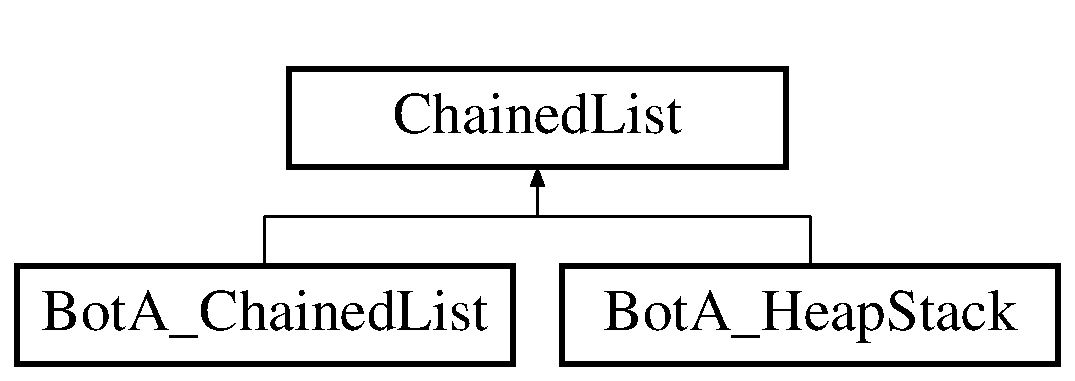
\includegraphics[height=2cm]{classChainedList}
\end{center}
\end{figure}
\subsection*{Public Member Functions}
\begin{CompactItemize}
\item 
{\bf ChainedList} ()
\item 
virtual {\bf $\sim$ChainedList} ()
\item 
virtual {\bf ListNode} $\ast$ {\bf getFirstItem} (void) const 
\item 
{\bf ListNode} $\ast$ {\bf getLastItem} (void) const 
\item 
int {\bf getLength} (void) const 
\item 
void {\bf setFirstItem} ({\bf ListNode} $\ast$item)
\item 
void {\bf setLastItem} ({\bf ListNode} $\ast$item)
\item 
void {\bf setLength} (int {\bf length})
\item 
virtual void {\bf addFirstItem} ({\bf TreeNode} $\ast$item)
\item 
virtual void {\bf addLastItem} ({\bf TreeNode} $\ast$item)
\item 
virtual void {\bf deleteFirstItem} (void)
\item 
virtual void {\bf deleteLastItem} (void)
\end{CompactItemize}
\subsection*{Protected Member Functions}
\begin{CompactItemize}
\item 
virtual {\bf ListNode} $\ast$ {\bf createListNode} ({\bf TreeNode} $\ast$treeNode)
\end{CompactItemize}
\subsection*{Protected Attributes}
\begin{CompactItemize}
\item 
{\bf ListNode} $\ast$ {\bf firstItem}
\item 
{\bf ListNode} $\ast$ {\bf lastItem}
\item 
int {\bf length}
\end{CompactItemize}


\subsection{Detailed Description}
Main Double Chained List of ListNodes class. 

This class contains informations about number of items in the list and first and last ListNodes. 

\subsection{Constructor \& Destructor Documentation}
\index{ChainedList@{ChainedList}!ChainedList@{ChainedList}}
\index{ChainedList@{ChainedList}!ChainedList@{ChainedList}}
\subsubsection{\setlength{\rightskip}{0pt plus 5cm}ChainedList::ChainedList ()}\label{classChainedList_db2f3a88c5443d6f60bed8aa99b48f12}


Constructor of an empty chained list \index{ChainedList@{ChainedList}!~ChainedList@{$\sim$ChainedList}}
\index{~ChainedList@{$\sim$ChainedList}!ChainedList@{ChainedList}}
\subsubsection{\setlength{\rightskip}{0pt plus 5cm}ChainedList::$\sim$ChainedList ()\hspace{0.3cm}{\tt  [virtual]}}\label{classChainedList_d01c2cd292e344e9ab28ecae01cf03f4}


Destructor 

\subsection{Member Function Documentation}
\index{ChainedList@{ChainedList}!getFirstItem@{getFirstItem}}
\index{getFirstItem@{getFirstItem}!ChainedList@{ChainedList}}
\subsubsection{\setlength{\rightskip}{0pt plus 5cm}virtual {\bf ListNode}$\ast$ ChainedList::getFirstItem (void) const\hspace{0.3cm}{\tt  [inline, virtual]}}\label{classChainedList_fb20aaef36ab32d23a35bb0c909715b2}


start item of the list 

Reimplemented in {\bf BotA\_\-HeapStack} \doxyref{}{p.}{classBotA__HeapStack_ebe93c0a849f73fa773e24ffc0aa16e8}.\index{ChainedList@{ChainedList}!getLastItem@{getLastItem}}
\index{getLastItem@{getLastItem}!ChainedList@{ChainedList}}
\subsubsection{\setlength{\rightskip}{0pt plus 5cm}{\bf ListNode}$\ast$ ChainedList::getLastItem (void) const\hspace{0.3cm}{\tt  [inline]}}\label{classChainedList_7a72e6df9bc5461d328292c7d4284b34}


last item of the list \index{ChainedList@{ChainedList}!getLength@{getLength}}
\index{getLength@{getLength}!ChainedList@{ChainedList}}
\subsubsection{\setlength{\rightskip}{0pt plus 5cm}int ChainedList::getLength (void) const\hspace{0.3cm}{\tt  [inline]}}\label{classChainedList_8cf0661ee6c0e0f6259cd2e487fe94ce}


length of the list 

Reimplemented in {\bf BotA\_\-HeapStack} \doxyref{}{p.}{classBotA__HeapStack_6d9feab2ffbaad17131a7151b308d051}.\index{ChainedList@{ChainedList}!setFirstItem@{setFirstItem}}
\index{setFirstItem@{setFirstItem}!ChainedList@{ChainedList}}
\subsubsection{\setlength{\rightskip}{0pt plus 5cm}void ChainedList::setFirstItem ({\bf ListNode} $\ast$ {\em item})\hspace{0.3cm}{\tt  [inline]}}\label{classChainedList_bcb3603d39cb01bb997162af2fad0b74}


start item of the list \index{ChainedList@{ChainedList}!setLastItem@{setLastItem}}
\index{setLastItem@{setLastItem}!ChainedList@{ChainedList}}
\subsubsection{\setlength{\rightskip}{0pt plus 5cm}void ChainedList::setLastItem ({\bf ListNode} $\ast$ {\em item})\hspace{0.3cm}{\tt  [inline]}}\label{classChainedList_aec0f918b6873a59cc03eb4168dd5a45}


last item of the list \index{ChainedList@{ChainedList}!setLength@{setLength}}
\index{setLength@{setLength}!ChainedList@{ChainedList}}
\subsubsection{\setlength{\rightskip}{0pt plus 5cm}void ChainedList::setLength (int {\em length})\hspace{0.3cm}{\tt  [inline]}}\label{classChainedList_64447d0e2c5ef2bdc2a0cfa0182b7294}


length of the list \index{ChainedList@{ChainedList}!addFirstItem@{addFirstItem}}
\index{addFirstItem@{addFirstItem}!ChainedList@{ChainedList}}
\subsubsection{\setlength{\rightskip}{0pt plus 5cm}void ChainedList::addFirstItem ({\bf TreeNode} $\ast$ {\em item})\hspace{0.3cm}{\tt  [virtual]}}\label{classChainedList_52ad982ab220ad0eea5513180f434db2}


Add an item to the end of the chainedlist \begin{Desc}
\item[Parameters:]
\begin{description}
\item[{\em item}]Item to add \end{description}
\end{Desc}


Reimplemented in {\bf BotA\_\-HeapStack} \doxyref{}{p.}{classBotA__HeapStack_7ab05ef7a0237229c5973e95cfcefc1c}.\index{ChainedList@{ChainedList}!addLastItem@{addLastItem}}
\index{addLastItem@{addLastItem}!ChainedList@{ChainedList}}
\subsubsection{\setlength{\rightskip}{0pt plus 5cm}void ChainedList::addLastItem ({\bf TreeNode} $\ast$ {\em item})\hspace{0.3cm}{\tt  [virtual]}}\label{classChainedList_92aa990058d417146bc43beed16c90f6}


Add an item to the end of the chainedlist \begin{Desc}
\item[Parameters:]
\begin{description}
\item[{\em item}]Item to add \end{description}
\end{Desc}


Reimplemented in {\bf BotA\_\-HeapStack} \doxyref{}{p.}{classBotA__HeapStack_aef3826b63645c27d10e7f673211fe94}.\index{ChainedList@{ChainedList}!deleteFirstItem@{deleteFirstItem}}
\index{deleteFirstItem@{deleteFirstItem}!ChainedList@{ChainedList}}
\subsubsection{\setlength{\rightskip}{0pt plus 5cm}void ChainedList::deleteFirstItem (void)\hspace{0.3cm}{\tt  [virtual]}}\label{classChainedList_01dc3f81d3a912ec2455734cdf2d1e46}


Delete first item of the list 

Reimplemented in {\bf BotA\_\-HeapStack} \doxyref{}{p.}{classBotA__HeapStack_798de6d8fe135f04a2d76a36eff147cd}.\index{ChainedList@{ChainedList}!deleteLastItem@{deleteLastItem}}
\index{deleteLastItem@{deleteLastItem}!ChainedList@{ChainedList}}
\subsubsection{\setlength{\rightskip}{0pt plus 5cm}void ChainedList::deleteLastItem (void)\hspace{0.3cm}{\tt  [virtual]}}\label{classChainedList_de017c8ad7cbfc4d347473bf303b1da2}


Delete last item of the list 

Reimplemented in {\bf BotA\_\-HeapStack} \doxyref{}{p.}{classBotA__HeapStack_3d787006c437d954881f2c3833b6190b}.\index{ChainedList@{ChainedList}!createListNode@{createListNode}}
\index{createListNode@{createListNode}!ChainedList@{ChainedList}}
\subsubsection{\setlength{\rightskip}{0pt plus 5cm}{\bf ListNode} $\ast$ ChainedList::createListNode ({\bf TreeNode} $\ast$ {\em treeNode})\hspace{0.3cm}{\tt  [protected, virtual]}}\label{classChainedList_fa807d5bcc23ab479f10a3771fb22735}


Create an \doxyref{ListNode}{p.}{classListNode} containing a treeNode \begin{Desc}
\item[Parameters:]
\begin{description}
\item[{\em treeNode}]\doxyref{TreeNode}{p.}{classTreeNode} to store in this \doxyref{ListNode}{p.}{classListNode} \end{description}
\end{Desc}
\begin{Desc}
\item[Returns:]New \doxyref{ListNode}{p.}{classListNode} filled with the treeNode argument \end{Desc}


Reimplemented in {\bf BotA\_\-ChainedList} \doxyref{}{p.}{classBotA__ChainedList_0d0aa702abdd01801e3262ba55ed9315}.

\subsection{Member Data Documentation}
\index{ChainedList@{ChainedList}!firstItem@{firstItem}}
\index{firstItem@{firstItem}!ChainedList@{ChainedList}}
\subsubsection{\setlength{\rightskip}{0pt plus 5cm}{\bf ListNode}$\ast$ {\bf ChainedList::firstItem}\hspace{0.3cm}{\tt  [protected]}}\label{classChainedList_c096cb50bfcdea95385bbd40bd0a7461}


first item pointer of the list \index{ChainedList@{ChainedList}!lastItem@{lastItem}}
\index{lastItem@{lastItem}!ChainedList@{ChainedList}}
\subsubsection{\setlength{\rightskip}{0pt plus 5cm}{\bf ListNode}$\ast$ {\bf ChainedList::lastItem}\hspace{0.3cm}{\tt  [protected]}}\label{classChainedList_466990a24511a304e69551fea36e017c}


last item pointer of the list \index{ChainedList@{ChainedList}!length@{length}}
\index{length@{length}!ChainedList@{ChainedList}}
\subsubsection{\setlength{\rightskip}{0pt plus 5cm}int {\bf ChainedList::length}\hspace{0.3cm}{\tt  [protected]}}\label{classChainedList_928bfe07dba537fd73937f1c0b369530}


length of the list 

The documentation for this class was generated from the following files:\begin{CompactItemize}
\item 
include/Solver/ChainedList.h\item 
src/Solver/ChainedList.cpp\end{CompactItemize}

\section{Data Class Reference}
\label{classData}\index{Data@{Data}}
Datas relative to game context.  


{\tt \#include $<$Data.h$>$}

\subsection*{Public Member Functions}
\begin{CompactItemize}
\item 
{\bf Data} (Base $\ast${\bf base}, int argc, char $\ast$const $\ast$const argv)
\item 
{\bf $\sim$Data} ()
\item 
{\bf StringList} $\ast$ {\bf getPackNameList} (void) const 
\item 
{\bf StringList} $\ast$ {\bf getPlayerNameList} (void) const 
\item 
int {\bf getSelectedPackNameId} (void) const 
\item 
int {\bf getSelectedPlayerNameId} (void) const 
\item 
char {\bf getScreenMode} (void) const 
\item 
int {\bf getWidth} (void) const 
\item 
int {\bf getHeight} (void) const 
\item 
const char $\ast$ {\bf getResolution} (void) const 
\item 
const char $\ast$ {\bf getLanguage} (void) const 
\item 
bool {\bf getSound} (void) const 
\item 
bool {\bf getMusic} (void) const 
\end{CompactItemize}
\subsection*{Protected Attributes}
\begin{CompactItemize}
\item 
Base $\ast$ {\bf base}
\item 
{\bf StringList} $\ast$ {\bf packNameList}
\item 
{\bf StringList} $\ast$ {\bf playerNameList}
\item 
int {\bf selectedPackNameId}
\item 
int {\bf selectedPlayerNameId}
\item 
char {\bf screenMode}
\item 
int {\bf width}
\item 
int {\bf height}
\item 
char $\ast$ {\bf resolution}
\item 
char $\ast$ {\bf language}
\item 
bool {\bf sound}
\item 
bool {\bf music}
\end{CompactItemize}


\subsection{Detailed Description}
Datas relative to game context. 

\subsection{Constructor \& Destructor Documentation}
\index{Data@{Data}!Data@{Data}}
\index{Data@{Data}!Data@{Data}}
\subsubsection{\setlength{\rightskip}{0pt plus 5cm}Data::Data (Base $\ast$ {\em base}, int {\em argc}, char $\ast$const $\ast$const  {\em argv})}\label{classData_e75d903f8aa84549e555d73733e2e3ea}


Constructor for game datas. \begin{Desc}
\item[Parameters:]
\begin{description}
\item[{\em base}]main class of the game \item[{\em argc}]number of arguments \item[{\em argv}]param starting params These are like this : ./sokoban \char`\"{}pseudo\char`\"{} -t \char`\"{}widthxheight\char`\"{} \char`\"{}fr\char`\"{} sound music t : w for windowed mode, f for fullscreen mode sound : 1=on 0=false music : 1=on 0=false example : ./sokoban \char`\"{}michael\char`\"{} -f \char`\"{}800x600\char`\"{} \char`\"{}fr\char`\"{} 1 1 \end{description}
\end{Desc}
\index{Data@{Data}!~Data@{$\sim$Data}}
\index{~Data@{$\sim$Data}!Data@{Data}}
\subsubsection{\setlength{\rightskip}{0pt plus 5cm}Data::$\sim$Data ()}\label{classData_ab31956423290f0d62dcca47ab4d16dd}


Destructor 

\subsection{Member Function Documentation}
\index{Data@{Data}!getPackNameList@{getPackNameList}}
\index{getPackNameList@{getPackNameList}!Data@{Data}}
\subsubsection{\setlength{\rightskip}{0pt plus 5cm}{\bf StringList}$\ast$ Data::getPackNameList (void) const\hspace{0.3cm}{\tt  [inline]}}\label{classData_975b98cc0209ec1e70af24c41ce06965}


list of pack names \index{Data@{Data}!getPlayerNameList@{getPlayerNameList}}
\index{getPlayerNameList@{getPlayerNameList}!Data@{Data}}
\subsubsection{\setlength{\rightskip}{0pt plus 5cm}{\bf StringList}$\ast$ Data::getPlayerNameList (void) const\hspace{0.3cm}{\tt  [inline]}}\label{classData_376cf46edec1f0e63f8a054497147e25}


list of player names \index{Data@{Data}!getSelectedPackNameId@{getSelectedPackNameId}}
\index{getSelectedPackNameId@{getSelectedPackNameId}!Data@{Data}}
\subsubsection{\setlength{\rightskip}{0pt plus 5cm}int Data::getSelectedPackNameId (void) const\hspace{0.3cm}{\tt  [inline]}}\label{classData_e86dd62d9fff6483bc5898f1f9f5030a}


id of selected pack in the list \index{Data@{Data}!getSelectedPlayerNameId@{getSelectedPlayerNameId}}
\index{getSelectedPlayerNameId@{getSelectedPlayerNameId}!Data@{Data}}
\subsubsection{\setlength{\rightskip}{0pt plus 5cm}int Data::getSelectedPlayerNameId (void) const\hspace{0.3cm}{\tt  [inline]}}\label{classData_e6655adbecaddaf9efc0e62bf3bcd69f}


id of selected player in the list \index{Data@{Data}!getScreenMode@{getScreenMode}}
\index{getScreenMode@{getScreenMode}!Data@{Data}}
\subsubsection{\setlength{\rightskip}{0pt plus 5cm}char Data::getScreenMode (void) const\hspace{0.3cm}{\tt  [inline]}}\label{classData_ee69054ed9720f8950b9ab8357a4bc6a}


Screen mode (windowed : w, fullscreen : f) \index{Data@{Data}!getWidth@{getWidth}}
\index{getWidth@{getWidth}!Data@{Data}}
\subsubsection{\setlength{\rightskip}{0pt plus 5cm}int Data::getWidth (void) const\hspace{0.3cm}{\tt  [inline]}}\label{classData_438bd9ad59a687ffcadf55a749e79d3d}


width of screen \index{Data@{Data}!getHeight@{getHeight}}
\index{getHeight@{getHeight}!Data@{Data}}
\subsubsection{\setlength{\rightskip}{0pt plus 5cm}int Data::getHeight (void) const\hspace{0.3cm}{\tt  [inline]}}\label{classData_26a94cc923971d4af5fdaa33c8202b31}


height of screen \index{Data@{Data}!getResolution@{getResolution}}
\index{getResolution@{getResolution}!Data@{Data}}
\subsubsection{\setlength{\rightskip}{0pt plus 5cm}const char$\ast$ Data::getResolution (void) const\hspace{0.3cm}{\tt  [inline]}}\label{classData_8c2685ee4b1d3a0f478a9c36b77ae6cb}


resolution of type \char`\"{}widthxheight\char`\"{} \index{Data@{Data}!getLanguage@{getLanguage}}
\index{getLanguage@{getLanguage}!Data@{Data}}
\subsubsection{\setlength{\rightskip}{0pt plus 5cm}const char$\ast$ Data::getLanguage (void) const\hspace{0.3cm}{\tt  [inline]}}\label{classData_e8352ffb87b12000ffdadcb138439b32}


language (\char`\"{}fr\char`\"{}, \char`\"{}en\char`\"{},..) \index{Data@{Data}!getSound@{getSound}}
\index{getSound@{getSound}!Data@{Data}}
\subsubsection{\setlength{\rightskip}{0pt plus 5cm}bool Data::getSound (void) const\hspace{0.3cm}{\tt  [inline]}}\label{classData_8e4a4fcd24d72ff76ee4fe64c9e96e7f}


true if sound is on, false if sound is off \index{Data@{Data}!getMusic@{getMusic}}
\index{getMusic@{getMusic}!Data@{Data}}
\subsubsection{\setlength{\rightskip}{0pt plus 5cm}bool Data::getMusic (void) const\hspace{0.3cm}{\tt  [inline]}}\label{classData_8c6b482b7456abbff4c55435a764d211}


true if music is on, false if music is off 

\subsection{Member Data Documentation}
\index{Data@{Data}!base@{base}}
\index{base@{base}!Data@{Data}}
\subsubsection{\setlength{\rightskip}{0pt plus 5cm}Base$\ast$ {\bf Data::base}\hspace{0.3cm}{\tt  [protected]}}\label{classData_3efc74fa4d74e869b3de1216a478093a}


Main class of the game \index{Data@{Data}!packNameList@{packNameList}}
\index{packNameList@{packNameList}!Data@{Data}}
\subsubsection{\setlength{\rightskip}{0pt plus 5cm}{\bf StringList}$\ast$ {\bf Data::packNameList}\hspace{0.3cm}{\tt  [protected]}}\label{classData_78e54e3ad4aa42193d305bcfef7c914e}


List of all available packs \index{Data@{Data}!playerNameList@{playerNameList}}
\index{playerNameList@{playerNameList}!Data@{Data}}
\subsubsection{\setlength{\rightskip}{0pt plus 5cm}{\bf StringList}$\ast$ {\bf Data::playerNameList}\hspace{0.3cm}{\tt  [protected]}}\label{classData_105f17586075d436b1ca8cc5347573c4}


List of all available players \index{Data@{Data}!selectedPackNameId@{selectedPackNameId}}
\index{selectedPackNameId@{selectedPackNameId}!Data@{Data}}
\subsubsection{\setlength{\rightskip}{0pt plus 5cm}int {\bf Data::selectedPackNameId}\hspace{0.3cm}{\tt  [protected]}}\label{classData_410fcdeb835be0020ecde93a37be1ea3}


Id of selected pack on the list \index{Data@{Data}!selectedPlayerNameId@{selectedPlayerNameId}}
\index{selectedPlayerNameId@{selectedPlayerNameId}!Data@{Data}}
\subsubsection{\setlength{\rightskip}{0pt plus 5cm}int {\bf Data::selectedPlayerNameId}\hspace{0.3cm}{\tt  [protected]}}\label{classData_f85b58b98b1d1c0b7cd8728ae0df0230}


Id of selected player on the list \index{Data@{Data}!screenMode@{screenMode}}
\index{screenMode@{screenMode}!Data@{Data}}
\subsubsection{\setlength{\rightskip}{0pt plus 5cm}char {\bf Data::screenMode}\hspace{0.3cm}{\tt  [protected]}}\label{classData_3ec26a33251799b0ef2d5761701f6bc2}


f for fullscreen mode, w for windowed mode \index{Data@{Data}!width@{width}}
\index{width@{width}!Data@{Data}}
\subsubsection{\setlength{\rightskip}{0pt plus 5cm}int {\bf Data::width}\hspace{0.3cm}{\tt  [protected]}}\label{classData_af3b89fcc4f2e12a58949b2658e24708}


Width of window \index{Data@{Data}!height@{height}}
\index{height@{height}!Data@{Data}}
\subsubsection{\setlength{\rightskip}{0pt plus 5cm}int {\bf Data::height}\hspace{0.3cm}{\tt  [protected]}}\label{classData_15b7471f8a89645cd371ac2b4ec639d2}


Height of window \index{Data@{Data}!resolution@{resolution}}
\index{resolution@{resolution}!Data@{Data}}
\subsubsection{\setlength{\rightskip}{0pt plus 5cm}char$\ast$ {\bf Data::resolution}\hspace{0.3cm}{\tt  [protected]}}\label{classData_3f1eedb27daa3de5cef9ec122e45b4bd}


Resolution on this shape : \char`\"{}widthxheight\char`\"{} \index{Data@{Data}!language@{language}}
\index{language@{language}!Data@{Data}}
\subsubsection{\setlength{\rightskip}{0pt plus 5cm}char$\ast$ {\bf Data::language}\hspace{0.3cm}{\tt  [protected]}}\label{classData_d887f480e9b65529a8cf5e758e2629ed}


language of the game \char`\"{}fr\char`\"{}, \char`\"{}en\char`\"{}, ... \index{Data@{Data}!sound@{sound}}
\index{sound@{sound}!Data@{Data}}
\subsubsection{\setlength{\rightskip}{0pt plus 5cm}bool {\bf Data::sound}\hspace{0.3cm}{\tt  [protected]}}\label{classData_1c495f77d4d32410c20567660b1a664c}


True if you want sound, false if you don't \index{Data@{Data}!music@{music}}
\index{music@{music}!Data@{Data}}
\subsubsection{\setlength{\rightskip}{0pt plus 5cm}bool {\bf Data::music}\hspace{0.3cm}{\tt  [protected]}}\label{classData_b08de3d1253a66a37ae6764c53dcf113}


True if you want music, false if you don't 

The documentation for this class was generated from the following files:\begin{CompactItemize}
\item 
include/Data.h\item 
src/Data.cpp\end{CompactItemize}

\section{HashTable Class Reference}
\label{classHashTable}\index{HashTable@{HashTable}}
Hash Table Class to store all level states.  


{\tt \#include $<$HashTable.h$>$}

Inheritance diagram for HashTable::\begin{figure}[H]
\begin{center}
\leavevmode
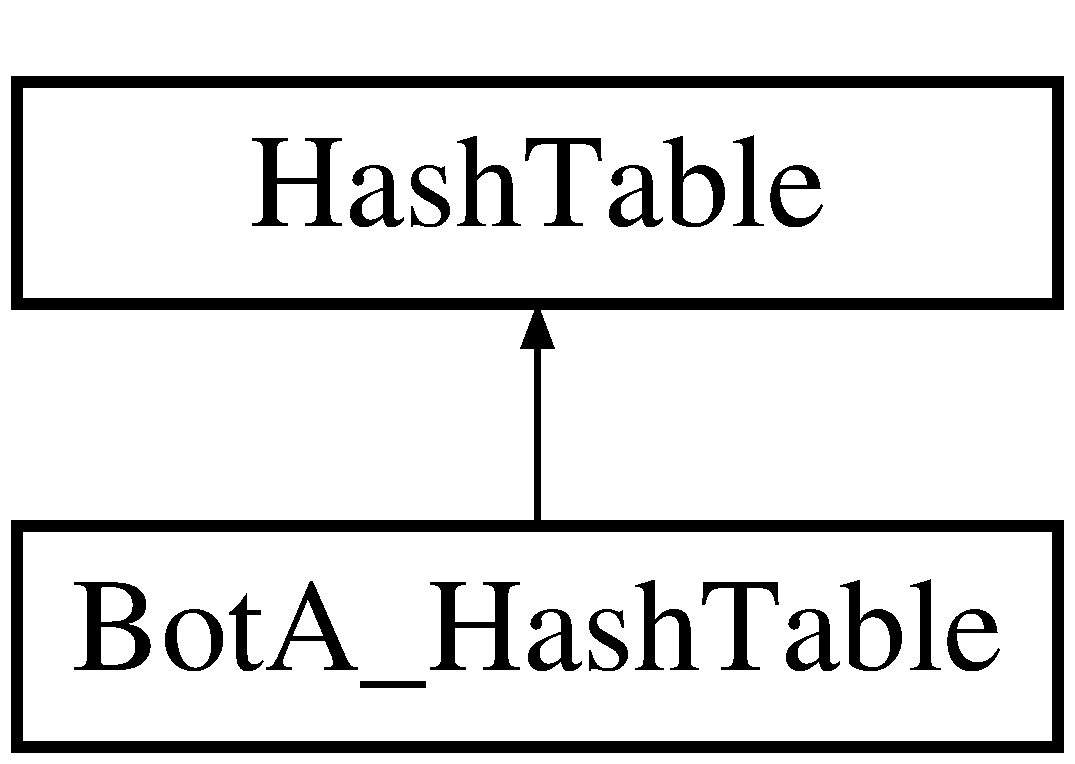
\includegraphics[height=2cm]{classHashTable}
\end{center}
\end{figure}
\subsection*{Public Member Functions}
\begin{CompactItemize}
\item 
{\bf HashTable} (int {\bf length})
\item 
virtual {\bf $\sim$HashTable} ()
\item 
{\bf ChainedList} $\ast$const $\ast$const {\bf getTable} (void) const 
\item 
int {\bf getLength} (void) const 
\item 
int {\bf getItemNumber} (void) const 
\item 
void {\bf addItem} ({\bf TreeNode} $\ast$treeNode)
\item 
bool {\bf removeItem} (const {\bf Node} $\ast$node)
\item 
virtual bool {\bf isPresent} (const {\bf Node} $\ast$node) const 
\item 
{\bf TreeNode} $\ast$ {\bf getTreeNodeFromNode} (const {\bf Node} $\ast$node)
\end{CompactItemize}
\subsection*{Protected Member Functions}
\begin{CompactItemize}
\item 
int {\bf h} (const {\bf Node} $\ast$node) const 
\end{CompactItemize}
\subsection*{Protected Attributes}
\begin{CompactItemize}
\item 
{\bf ChainedList} $\ast$$\ast$ {\bf table}
\item 
int {\bf length}
\item 
int {\bf itemNumber}
\end{CompactItemize}


\subsection{Detailed Description}
Hash Table Class to store all level states. 

This hash table is a tab of N \doxyref{ChainedList}{p.}{classChainedList} of \doxyref{TreeNode}{p.}{classTreeNode} (reuse of the processing tree pointer). when adding a \doxyref{TreeNode}{p.}{classTreeNode}, the \char`\"{}H\char`\"{} function is used to make a position in the tab from the node. 

\subsection{Constructor \& Destructor Documentation}
\index{HashTable@{HashTable}!HashTable@{HashTable}}
\index{HashTable@{HashTable}!HashTable@{HashTable}}
\subsubsection{\setlength{\rightskip}{0pt plus 5cm}HashTable::HashTable (int {\em length})}\label{classHashTable_43df4a83799c4af99ec07a16b354bbb0}


Constructor \index{HashTable@{HashTable}!~HashTable@{$\sim$HashTable}}
\index{~HashTable@{$\sim$HashTable}!HashTable@{HashTable}}
\subsubsection{\setlength{\rightskip}{0pt plus 5cm}HashTable::$\sim$HashTable ()\hspace{0.3cm}{\tt  [virtual]}}\label{classHashTable_9ce5569bb945880cacb29aaba6f3e3f9}


Destructor 

\subsection{Member Function Documentation}
\index{HashTable@{HashTable}!getTable@{getTable}}
\index{getTable@{getTable}!HashTable@{HashTable}}
\subsubsection{\setlength{\rightskip}{0pt plus 5cm}{\bf ChainedList}$\ast$ const$\ast$ const HashTable::getTable (void) const\hspace{0.3cm}{\tt  [inline]}}\label{classHashTable_fc8bb0f016829e3b3686caf8b78241a3}


table of \char`\"{}length\char`\"{} chainedlist \index{HashTable@{HashTable}!getLength@{getLength}}
\index{getLength@{getLength}!HashTable@{HashTable}}
\subsubsection{\setlength{\rightskip}{0pt plus 5cm}int HashTable::getLength (void) const\hspace{0.3cm}{\tt  [inline]}}\label{classHashTable_c23c225e5b23bf616a8fc7b16c4e9582}


length of table \index{HashTable@{HashTable}!getItemNumber@{getItemNumber}}
\index{getItemNumber@{getItemNumber}!HashTable@{HashTable}}
\subsubsection{\setlength{\rightskip}{0pt plus 5cm}int HashTable::getItemNumber (void) const\hspace{0.3cm}{\tt  [inline]}}\label{classHashTable_6fcecb1808a92d3aef69bbe578241314}


number of items stocked in the hashtable \index{HashTable@{HashTable}!addItem@{addItem}}
\index{addItem@{addItem}!HashTable@{HashTable}}
\subsubsection{\setlength{\rightskip}{0pt plus 5cm}void HashTable::addItem ({\bf TreeNode} $\ast$ {\em treeNode})}\label{classHashTable_9b6497cfeedd59f8327aa99d0bb35de2}


Add an item into the table but don't test if it is already present \begin{Desc}
\item[Parameters:]
\begin{description}
\item[{\em treeNode}]treeNode pointer we want to add to the hashTable \end{description}
\end{Desc}
\index{HashTable@{HashTable}!removeItem@{removeItem}}
\index{removeItem@{removeItem}!HashTable@{HashTable}}
\subsubsection{\setlength{\rightskip}{0pt plus 5cm}bool HashTable::removeItem (const {\bf Node} $\ast$ {\em node})}\label{classHashTable_6701637e1a3bb03ba85b666dcc283190}


Delete an item from the table (if this item if several times in the table, we delete it only one time). It delete only listNode but pointer to treeNode stay in the tree \begin{Desc}
\item[Parameters:]
\begin{description}
\item[{\em node}]\doxyref{Node}{p.}{classNode} we want to delete from the table \end{description}
\end{Desc}
\begin{Desc}
\item[Returns:]true if something was deleted, false if not \end{Desc}
\index{HashTable@{HashTable}!isPresent@{isPresent}}
\index{isPresent@{isPresent}!HashTable@{HashTable}}
\subsubsection{\setlength{\rightskip}{0pt plus 5cm}bool HashTable::isPresent (const {\bf Node} $\ast$ {\em node}) const\hspace{0.3cm}{\tt  [virtual]}}\label{classHashTable_1a1b16b0cfd69e0771cb55fe802229eb}


Test if an \doxyref{Node}{p.}{classNode} is already present into the hashTable \begin{Desc}
\item[Parameters:]
\begin{description}
\item[{\em node}]\doxyref{Node}{p.}{classNode} we want to test \end{description}
\end{Desc}
\begin{Desc}
\item[Returns:]true if the \doxyref{Node}{p.}{classNode} is present, false if not \end{Desc}


Reimplemented in {\bf BotA\_\-HashTable} \doxyref{}{p.}{classBotA__HashTable_e6005e8a8ed9551f640ecd325a8165f8}.\index{HashTable@{HashTable}!getTreeNodeFromNode@{getTreeNodeFromNode}}
\index{getTreeNodeFromNode@{getTreeNodeFromNode}!HashTable@{HashTable}}
\subsubsection{\setlength{\rightskip}{0pt plus 5cm}{\bf TreeNode} $\ast$ HashTable::getTreeNodeFromNode (const {\bf Node} $\ast$ {\em node})}\label{classHashTable_d21e933a903e865ca5a82b2938f357f8}


Get a treenode pointer in hashtable from a node \begin{Desc}
\item[Parameters:]
\begin{description}
\item[{\em node}]\doxyref{Node}{p.}{classNode} we want use to find treenode \end{description}
\end{Desc}
\begin{Desc}
\item[Returns:]treenode pointer to found node or NULL if node doesn't exist in hashtable \end{Desc}
\index{HashTable@{HashTable}!h@{h}}
\index{h@{h}!HashTable@{HashTable}}
\subsubsection{\setlength{\rightskip}{0pt plus 5cm}int HashTable::h (const {\bf Node} $\ast$ {\em node}) const\hspace{0.3cm}{\tt  [protected]}}\label{classHashTable_ac4876a25e566f3d22e691ea2f99e0cd}


Hashing function that use a node to compute an index number for the tab \begin{Desc}
\item[Parameters:]
\begin{description}
\item[{\em node}]\doxyref{Node}{p.}{classNode} we want to compute \end{description}
\end{Desc}
\begin{Desc}
\item[Returns:]index number for the tab \end{Desc}


\subsection{Member Data Documentation}
\index{HashTable@{HashTable}!table@{table}}
\index{table@{table}!HashTable@{HashTable}}
\subsubsection{\setlength{\rightskip}{0pt plus 5cm}{\bf ChainedList}$\ast$$\ast$ {\bf HashTable::table}\hspace{0.3cm}{\tt  [protected]}}\label{classHashTable_4071126e173ebb8b71a8241713e290ed}


Table of hashing \index{HashTable@{HashTable}!length@{length}}
\index{length@{length}!HashTable@{HashTable}}
\subsubsection{\setlength{\rightskip}{0pt plus 5cm}int {\bf HashTable::length}\hspace{0.3cm}{\tt  [protected]}}\label{classHashTable_28d1b9720c344d5faf4da89c3a6a6041}


Length of hashtable : number of cells \index{HashTable@{HashTable}!itemNumber@{itemNumber}}
\index{itemNumber@{itemNumber}!HashTable@{HashTable}}
\subsubsection{\setlength{\rightskip}{0pt plus 5cm}int {\bf HashTable::itemNumber}\hspace{0.3cm}{\tt  [protected]}}\label{classHashTable_313d93108fd540454a433f9bba3c4fa3}


Number of items in the table 

The documentation for this class was generated from the following files:\begin{CompactItemize}
\item 
include/Solver/HashTable.h\item 
src/Solver/HashTable.cpp\end{CompactItemize}

\section{Level Class Reference}
\label{classLevel}\index{Level@{Level}}
Class containing a level and every functions about it.  


{\tt \#include $<$Level.h$>$}

\subsection*{Public Member Functions}
\begin{CompactItemize}
\item 
{\bf Level} (Base $\ast${\bf base})
\item 
{\bf Level} (Base $\ast${\bf base}, const {\bf Level} $\ast$source)
\item 
{\bf Level} (Base $\ast${\bf base}, xmlNodePtr levelNode, xmlNodePtr pathNode, int {\bf id}, const char $\ast${\bf packName})
\item 
{\bf $\sim$Level} ()
\item 
int {\bf getId} (void) const 
\item 
const char $\ast$ {\bf getName} (void) const 
\item 
const char $\ast$ {\bf getPackName} (void) const 
\item 
const char $\ast$ {\bf getGrid} (void) const 
\item 
int {\bf getBoxesNumber} (void) const 
\item 
int {\bf getGoalsNumber} (void) const 
\item 
int {\bf getRowsNumber} (void) const 
\item 
int {\bf getColsNumber} (void) const 
\item 
int {\bf getPusherPosM} (void) const 
\item 
int {\bf getPusherPosN} (void) const 
\item 
double {\bf getXCenter} (void) const 
\item 
double {\bf getYCenter} (void) const 
\item 
bool {\bf getWon} (void) const 
\item 
const {\bf Path} $\ast$ {\bf getMyBestMoves} (void) const 
\item 
const {\bf Path} $\ast$ {\bf getMyBestPushes} (void) const 
\item 
const {\bf Path} $\ast$ {\bf getWorldBestMoves} (void) const 
\item 
const {\bf Path} $\ast$ {\bf getWorldBestPushes} (void) const 
\item 
{\bf Path} $\ast$ {\bf getActualPath} (void) const 
\item 
void {\bf setBoxesNumber} (int {\bf boxesNumber})
\item 
void {\bf setGoalsNumber} (int {\bf goalsNumber})
\item 
void {\bf setPusherPosM} (int {\bf pusherPosM})
\item 
void {\bf setPusherPosN} (int {\bf pusherPosN})
\item 
char {\bf readPos} (const int m, const int n) const 
\item 
char {\bf readPos} (const int pos) const 
\item 
void {\bf writePos} (const int m, const int n, const char letter)
\item 
void {\bf writePos} (const int pos, const char letter)
\item 
bool {\bf pusherCanMove} (const char direction) const 
\item 
int {\bf move} (const char direction)
\item 
int {\bf eraseMove} (void)
\item 
bool {\bf isWon} (void) const 
\item 
bool {\bf isSolution} ({\bf Path} $\ast$path) const 
\item 
void {\bf print} (const char $\ast$fileName) const 
\item 
void {\bf print} (void) const 
\item 
void {\bf xmlSavePath} (FILE $\ast$file) const 
\end{CompactItemize}
\subsection*{Protected Member Functions}
\begin{CompactItemize}
\item 
void {\bf initializePusherPos} (void)
\item 
void {\bf makeGround} (void)
\item 
void {\bf makeGroundRec} (const int m, const int n)
\item 
void {\bf copyLevel} (const {\bf Level} $\ast$source)
\item 
void {\bf printInFile} (const char $\ast$fileName) const 
\item 
void {\bf xmlLoad} (xmlNodePtr levelNode, xmlNodePtr pathNode, const int {\bf id})
\end{CompactItemize}
\subsection*{Protected Attributes}
\begin{CompactItemize}
\item 
Base $\ast$ {\bf base}
\item 
int {\bf id}
\item 
char {\bf name} [65]
\item 
char {\bf packName} [33]
\item 
char $\ast$ {\bf grid}
\item 
int {\bf boxesNumber}
\item 
int {\bf goalsNumber}
\item 
int {\bf rowsNumber}
\item 
int {\bf colsNumber}
\item 
int {\bf pusherPosM}
\item 
int {\bf pusherPosN}
\item 
double {\bf xCenter}
\item 
double {\bf yCenter}
\item 
bool {\bf won}
\item 
{\bf Path} $\ast$ {\bf myBestMoves}
\item 
{\bf Path} $\ast$ {\bf myBestPushes}
\item 
{\bf Path} $\ast$ {\bf worldBestMoves}
\item 
{\bf Path} $\ast$ {\bf worldBestPushes}
\item 
{\bf Path} $\ast$ {\bf actualPath}
\end{CompactItemize}


\subsection{Detailed Description}
Class containing a level and every functions about it. 

Positions in grid start in the upper-left corner with (m=0,n=0).

Example : (2,4) means third rows and fifth cols starting in the upper-left corner.

Grid is made like this in loaded files :

\#\#\#\#\# \# -$>$ wall \# \# \$ -$>$ box \#\$ \# . -$>$ goal \#\#\# \$\#\# $\ast$ -$>$ box on a goal (not in this figure) \# \$ \$ \# @ -$>$ pusher \#\#\# \# \#\# \# \#\#\#\#\#\# + -$>$ pusher on a goal \# \# \#\# \#\#\#\#\# ..\# s -$>$ inside ground (generated by recursive \# \$ \$ ..\# algorithm in program memory \#\#\#\#\# \#\#\# \#\#\# ..\# \# \#\#\#\#\#\#\#\#\# \#\#\#\#\#\#\# 

\subsection{Constructor \& Destructor Documentation}
\index{Level@{Level}!Level@{Level}}
\index{Level@{Level}!Level@{Level}}
\subsubsection{\setlength{\rightskip}{0pt plus 5cm}Level::Level (Base $\ast$ {\em base})}\label{classLevel_63852119715bd4c4fb6bc43540a9610b}


Constructor for a empty level \begin{Desc}
\item[Parameters:]
\begin{description}
\item[{\em base}]main class of the game \end{description}
\end{Desc}
\index{Level@{Level}!Level@{Level}}
\index{Level@{Level}!Level@{Level}}
\subsubsection{\setlength{\rightskip}{0pt plus 5cm}Level::Level (Base $\ast$ {\em base}, const {\bf Level} $\ast$ {\em source})}\label{classLevel_b069223ec6ef8b05fd22d0d3e52dddaa}


Constructor for a level which is copy of param \char`\"{}level\char`\"{} \begin{Desc}
\item[Parameters:]
\begin{description}
\item[{\em base}]main class of the game \item[{\em source}]to be copied in this object \end{description}
\end{Desc}
\index{Level@{Level}!Level@{Level}}
\index{Level@{Level}!Level@{Level}}
\subsubsection{\setlength{\rightskip}{0pt plus 5cm}Level::Level (Base $\ast$ {\em base}, xmlNodePtr {\em levelNode}, xmlNodePtr {\em pathNode}, int {\em id}, const char $\ast$ {\em packName})}\label{classLevel_f159d10cbb7c96eb2970386dd6cdf141}


Constructor for a level from a \doxyref{Node}{p.}{classNode} in a XML sile \begin{Desc}
\item[Parameters:]
\begin{description}
\item[{\em base}]main class of the game \item[{\em levelNode}]\doxyref{Node}{p.}{classNode} in XML file containing levels \item[{\em pathNode}]\doxyref{Node}{p.}{classNode} in XML file containing paths of loggued player \item[{\em id}]number of this level in its pack (starting with 1) \item[{\em Name}]of the pack that contains this level \end{description}
\end{Desc}
\index{Level@{Level}!~Level@{$\sim$Level}}
\index{~Level@{$\sim$Level}!Level@{Level}}
\subsubsection{\setlength{\rightskip}{0pt plus 5cm}Level::$\sim$Level ()}\label{classLevel_249eac1e8f19ff44134efa5e986feaca}


Destructor 

\subsection{Member Function Documentation}
\index{Level@{Level}!getId@{getId}}
\index{getId@{getId}!Level@{Level}}
\subsubsection{\setlength{\rightskip}{0pt plus 5cm}int Level::getId (void) const\hspace{0.3cm}{\tt  [inline]}}\label{classLevel_c524db3d97809670353b769d489d2193}


Id of this level \index{Level@{Level}!getName@{getName}}
\index{getName@{getName}!Level@{Level}}
\subsubsection{\setlength{\rightskip}{0pt plus 5cm}const char$\ast$ Level::getName (void) const\hspace{0.3cm}{\tt  [inline]}}\label{classLevel_8f5b8cbd7760eac49d57c5b37672ef34}


Name of this level \index{Level@{Level}!getPackName@{getPackName}}
\index{getPackName@{getPackName}!Level@{Level}}
\subsubsection{\setlength{\rightskip}{0pt plus 5cm}const char$\ast$ Level::getPackName (void) const\hspace{0.3cm}{\tt  [inline]}}\label{classLevel_fd86f5671ac63b1f64dad9b1aebca1e2}


Name of pack that contains this level \index{Level@{Level}!getGrid@{getGrid}}
\index{getGrid@{getGrid}!Level@{Level}}
\subsubsection{\setlength{\rightskip}{0pt plus 5cm}const char$\ast$ Level::getGrid (void) const\hspace{0.3cm}{\tt  [inline]}}\label{classLevel_98df93613a32105446ff75986fc86393}


Grid of this level \index{Level@{Level}!getBoxesNumber@{getBoxesNumber}}
\index{getBoxesNumber@{getBoxesNumber}!Level@{Level}}
\subsubsection{\setlength{\rightskip}{0pt plus 5cm}int Level::getBoxesNumber (void) const\hspace{0.3cm}{\tt  [inline]}}\label{classLevel_ecd2a23f61002a8cedbc8834eec296f7}


Number of boxes of this level \index{Level@{Level}!getGoalsNumber@{getGoalsNumber}}
\index{getGoalsNumber@{getGoalsNumber}!Level@{Level}}
\subsubsection{\setlength{\rightskip}{0pt plus 5cm}int Level::getGoalsNumber (void) const\hspace{0.3cm}{\tt  [inline]}}\label{classLevel_bbe0e39e2691cbb7458dc7ee08364cb4}


Number of goals of this level \index{Level@{Level}!getRowsNumber@{getRowsNumber}}
\index{getRowsNumber@{getRowsNumber}!Level@{Level}}
\subsubsection{\setlength{\rightskip}{0pt plus 5cm}int Level::getRowsNumber (void) const\hspace{0.3cm}{\tt  [inline]}}\label{classLevel_c984b30a9c2ab1464563163f99eb6e9d}


Number of rows of this level \index{Level@{Level}!getColsNumber@{getColsNumber}}
\index{getColsNumber@{getColsNumber}!Level@{Level}}
\subsubsection{\setlength{\rightskip}{0pt plus 5cm}int Level::getColsNumber (void) const\hspace{0.3cm}{\tt  [inline]}}\label{classLevel_00b681f2b47a0c38020840f7b1efcfb4}


Number of cols of this level \index{Level@{Level}!getPusherPosM@{getPusherPosM}}
\index{getPusherPosM@{getPusherPosM}!Level@{Level}}
\subsubsection{\setlength{\rightskip}{0pt plus 5cm}int Level::getPusherPosM (void) const\hspace{0.3cm}{\tt  [inline]}}\label{classLevel_5d374ba0ba8f58bc76a673914f861424}


pos of pusher (number of row) \index{Level@{Level}!getPusherPosN@{getPusherPosN}}
\index{getPusherPosN@{getPusherPosN}!Level@{Level}}
\subsubsection{\setlength{\rightskip}{0pt plus 5cm}int Level::getPusherPosN (void) const\hspace{0.3cm}{\tt  [inline]}}\label{classLevel_3f71af0793c7f631254c6cd02d07ec5d}


pos of pusher (number of col) \index{Level@{Level}!getXCenter@{getXCenter}}
\index{getXCenter@{getXCenter}!Level@{Level}}
\subsubsection{\setlength{\rightskip}{0pt plus 5cm}double Level::getXCenter (void) const\hspace{0.3cm}{\tt  [inline]}}\label{classLevel_cfcd92ae9a186deb77528bceac873a08}


X Center of this level (help to draw) \index{Level@{Level}!getYCenter@{getYCenter}}
\index{getYCenter@{getYCenter}!Level@{Level}}
\subsubsection{\setlength{\rightskip}{0pt plus 5cm}double Level::getYCenter (void) const\hspace{0.3cm}{\tt  [inline]}}\label{classLevel_995fcd9fe88ebf717498916b8a07f1f8}


Y Center of this level (help to draw) \index{Level@{Level}!getWon@{getWon}}
\index{getWon@{getWon}!Level@{Level}}
\subsubsection{\setlength{\rightskip}{0pt plus 5cm}bool Level::getWon (void) const\hspace{0.3cm}{\tt  [inline]}}\label{classLevel_1f73deaa9ec03c82b4343fb4a78c9eb2}


true if level is succeed, false if not \index{Level@{Level}!getMyBestMoves@{getMyBestMoves}}
\index{getMyBestMoves@{getMyBestMoves}!Level@{Level}}
\subsubsection{\setlength{\rightskip}{0pt plus 5cm}const {\bf Path}$\ast$ Level::getMyBestMoves (void) const\hspace{0.3cm}{\tt  [inline]}}\label{classLevel_38ef6bc511f65989b862c5b35b701304}


best moves of loggued player \index{Level@{Level}!getMyBestPushes@{getMyBestPushes}}
\index{getMyBestPushes@{getMyBestPushes}!Level@{Level}}
\subsubsection{\setlength{\rightskip}{0pt plus 5cm}const {\bf Path}$\ast$ Level::getMyBestPushes (void) const\hspace{0.3cm}{\tt  [inline]}}\label{classLevel_335041abc39d435e0cdce8bf56b9f1d7}


best pushes of loggued player \index{Level@{Level}!getWorldBestMoves@{getWorldBestMoves}}
\index{getWorldBestMoves@{getWorldBestMoves}!Level@{Level}}
\subsubsection{\setlength{\rightskip}{0pt plus 5cm}const {\bf Path}$\ast$ Level::getWorldBestMoves (void) const\hspace{0.3cm}{\tt  [inline]}}\label{classLevel_67304ea76a19b542fbc1e70d5d630b7d}


World best moves \index{Level@{Level}!getWorldBestPushes@{getWorldBestPushes}}
\index{getWorldBestPushes@{getWorldBestPushes}!Level@{Level}}
\subsubsection{\setlength{\rightskip}{0pt plus 5cm}const {\bf Path}$\ast$ Level::getWorldBestPushes (void) const\hspace{0.3cm}{\tt  [inline]}}\label{classLevel_a8c7674a5134917403530fdbd8ce2151}


World best pushes \index{Level@{Level}!getActualPath@{getActualPath}}
\index{getActualPath@{getActualPath}!Level@{Level}}
\subsubsection{\setlength{\rightskip}{0pt plus 5cm}{\bf Path}$\ast$ Level::getActualPath (void) const\hspace{0.3cm}{\tt  [inline]}}\label{classLevel_09ca2d4b843dd8e078597f1dd90e850b}


Actual path used in this level \index{Level@{Level}!setBoxesNumber@{setBoxesNumber}}
\index{setBoxesNumber@{setBoxesNumber}!Level@{Level}}
\subsubsection{\setlength{\rightskip}{0pt plus 5cm}void Level::setBoxesNumber (int {\em boxesNumber})\hspace{0.3cm}{\tt  [inline]}}\label{classLevel_fa3335731601b05b6c277b4235a14c57}


\begin{Desc}
\item[Parameters:]
\begin{description}
\item[{\em Number}]of boxes of this level \end{description}
\end{Desc}
\index{Level@{Level}!setGoalsNumber@{setGoalsNumber}}
\index{setGoalsNumber@{setGoalsNumber}!Level@{Level}}
\subsubsection{\setlength{\rightskip}{0pt plus 5cm}void Level::setGoalsNumber (int {\em goalsNumber})\hspace{0.3cm}{\tt  [inline]}}\label{classLevel_862a5e3c5c06a99dca9c0f5cfc6640d5}


\begin{Desc}
\item[Parameters:]
\begin{description}
\item[{\em Number}]of goals of this level \end{description}
\end{Desc}
\index{Level@{Level}!setPusherPosM@{setPusherPosM}}
\index{setPusherPosM@{setPusherPosM}!Level@{Level}}
\subsubsection{\setlength{\rightskip}{0pt plus 5cm}void Level::setPusherPosM (int {\em pusherPosM})\hspace{0.3cm}{\tt  [inline]}}\label{classLevel_eafbcc0d305acd4a87425aa09b57924a}


\begin{Desc}
\item[Parameters:]
\begin{description}
\item[{\em Number}]of rows of this level \end{description}
\end{Desc}
\index{Level@{Level}!setPusherPosN@{setPusherPosN}}
\index{setPusherPosN@{setPusherPosN}!Level@{Level}}
\subsubsection{\setlength{\rightskip}{0pt plus 5cm}void Level::setPusherPosN (int {\em pusherPosN})\hspace{0.3cm}{\tt  [inline]}}\label{classLevel_d306531d3b2c54c87634bfeb50a6b6a9}


\begin{Desc}
\item[Parameters:]
\begin{description}
\item[{\em Number}]of cols of this level \end{description}
\end{Desc}
\index{Level@{Level}!readPos@{readPos}}
\index{readPos@{readPos}!Level@{Level}}
\subsubsection{\setlength{\rightskip}{0pt plus 5cm}char Level::readPos (const int {\em m}, const int {\em n}) const}\label{classLevel_687c652f38cc52a762654e22d69b3fd2}


Read the value of position (m,n). Position start in the upper-left corner of the grid with (0,0). \begin{Desc}
\item[Parameters:]
\begin{description}
\item[{\em m}]Row number. \item[{\em n}]Col number. \end{description}
\end{Desc}
\begin{Desc}
\item[Returns:]Value of position (m,n) or 'E' if pos is out of grid. \end{Desc}
\index{Level@{Level}!readPos@{readPos}}
\index{readPos@{readPos}!Level@{Level}}
\subsubsection{\setlength{\rightskip}{0pt plus 5cm}char Level::readPos (const int {\em pos}) const}\label{classLevel_6ac14895acf881b97caa7e6f0c94b072}


Read the value of position \char`\"{}pos\char`\"{} of the grid. Position start in the upper-left corner of the grid with (0,0). \begin{Desc}
\item[Parameters:]
\begin{description}
\item[{\em pos}]Absolute position in the grid \end{description}
\end{Desc}
\begin{Desc}
\item[Returns:]Value of position pos or 'E' if pos is out of grid. \end{Desc}
\index{Level@{Level}!writePos@{writePos}}
\index{writePos@{writePos}!Level@{Level}}
\subsubsection{\setlength{\rightskip}{0pt plus 5cm}void Level::writePos (const int {\em m}, const int {\em n}, const char {\em letter})}\label{classLevel_74650865854bf496e4d523a48c08faf2}


Write the value of letter in position (m,n). Position start in the upper-left corner of the grid with (0,0). \begin{Desc}
\item[Parameters:]
\begin{description}
\item[{\em m}]Row number. \item[{\em n}]Col number. \item[{\em letter}]value to assign at (m,n) in the grid \end{description}
\end{Desc}
\index{Level@{Level}!writePos@{writePos}}
\index{writePos@{writePos}!Level@{Level}}
\subsubsection{\setlength{\rightskip}{0pt plus 5cm}void Level::writePos (const int {\em pos}, const char {\em letter})}\label{classLevel_bcd02d53f540160d0efe2ce5fe5e7441}


Write the value of letter in position \char`\"{}pos\char`\"{}. Position start in the upper-left corner of the grid with (0,0). \begin{Desc}
\item[Parameters:]
\begin{description}
\item[{\em pos}]Absolute position in the grid. \item[{\em letter}]value to assign at (m,n) in the grid \end{description}
\end{Desc}
\index{Level@{Level}!pusherCanMove@{pusherCanMove}}
\index{pusherCanMove@{pusherCanMove}!Level@{Level}}
\subsubsection{\setlength{\rightskip}{0pt plus 5cm}bool Level::pusherCanMove (const char {\em direction}) const}\label{classLevel_3f16cb3e5712d6d263ad5496f8c6e616}


Look if pusher can move in a given direction \begin{Desc}
\item[Parameters:]
\begin{description}
\item[{\em direction}]'u', 'd', 'l', 'r' in lowercase and uppercase \end{description}
\end{Desc}
\begin{Desc}
\item[Returns:]true if pusher can move in this direction, false if not. \end{Desc}
\index{Level@{Level}!move@{move}}
\index{move@{move}!Level@{Level}}
\subsubsection{\setlength{\rightskip}{0pt plus 5cm}int Level::move (const char {\em direction})}\label{classLevel_938645cb2d3844078b3d05de784c1a8a}


Move the pusher in a given direction and save it in the actualPath \begin{Desc}
\item[Parameters:]
\begin{description}
\item[{\em direction}]Direction where to move the pusher (u,d,l,r,U,D,L,R) \end{description}
\end{Desc}
\begin{Desc}
\item[Returns:]Level::MOUV\_\-NONE if no move. Level::MOUV\_\-SOKOBAN if normal move. Level::MOUV\_\-BOX if box move. \end{Desc}
\index{Level@{Level}!eraseMove@{eraseMove}}
\index{eraseMove@{eraseMove}!Level@{Level}}
\subsubsection{\setlength{\rightskip}{0pt plus 5cm}int Level::eraseMove (void)}\label{classLevel_0ffcf9100bca4e7232731fef133dbf53}


Move the pusher backward and erase last move in the actualPath \begin{Desc}
\item[Returns:]Level::MOUV\_\-NONE if no move. Level::MOUV\_\-SOKOBAN if normal move. Level::MOUV\_\-BOX if box move. \end{Desc}
\index{Level@{Level}!isWon@{isWon}}
\index{isWon@{isWon}!Level@{Level}}
\subsubsection{\setlength{\rightskip}{0pt plus 5cm}bool Level::isWon (void) const}\label{classLevel_31451ffc6dc5a30db52c40900025989f}


Return true if all boxes are in their goals. \begin{Desc}
\item[Returns:]true if all boxes are in their goals, false if not \end{Desc}
\index{Level@{Level}!isSolution@{isSolution}}
\index{isSolution@{isSolution}!Level@{Level}}
\subsubsection{\setlength{\rightskip}{0pt plus 5cm}bool Level::isSolution ({\bf Path} $\ast$ {\em path}) const}\label{classLevel_dcf29659bfee01c7af0aba90fc5abc32}


Test if a given path is solution of the ACTUAL STATE of this level \begin{Desc}
\item[Parameters:]
\begin{description}
\item[{\em path}]path to test in this level \end{description}
\end{Desc}
\begin{Desc}
\item[Returns:]true if path is solution, false if not. \end{Desc}
\index{Level@{Level}!print@{print}}
\index{print@{print}!Level@{Level}}
\subsubsection{\setlength{\rightskip}{0pt plus 5cm}void Level::print (const char $\ast$ {\em fileName}) const}\label{classLevel_3589df31fcc300ea419629027e0e6971}


Print level in text mode in a file. \begin{Desc}
\item[Parameters:]
\begin{description}
\item[{\em fileName}]name of the file we want to print in. \end{description}
\end{Desc}
\index{Level@{Level}!print@{print}}
\index{print@{print}!Level@{Level}}
\subsubsection{\setlength{\rightskip}{0pt plus 5cm}void Level::print (void) const}\label{classLevel_bc65fa529c6df10be43c2e9f3df0e187}


Print level in standard output \index{Level@{Level}!xmlSavePath@{xmlSavePath}}
\index{xmlSavePath@{xmlSavePath}!Level@{Level}}
\subsubsection{\setlength{\rightskip}{0pt plus 5cm}void Level::xmlSavePath (FILE $\ast$ {\em file}) const}\label{classLevel_4859e6d0f95e1199ff62e5cf7c53a85f}


Print every paths of this level in a openened file in parameter. You usually don't need to use this function (only with \doxyref{Pack::xmlSavePath()}{p.}{classPack_56bd1769b4478614a2dfe62e526b1fc8}). \begin{Desc}
\item[Parameters:]
\begin{description}
\item[{\em file}]opened file \end{description}
\end{Desc}
\index{Level@{Level}!initializePusherPos@{initializePusherPos}}
\index{initializePusherPos@{initializePusherPos}!Level@{Level}}
\subsubsection{\setlength{\rightskip}{0pt plus 5cm}void Level::initializePusherPos (void)\hspace{0.3cm}{\tt  [protected]}}\label{classLevel_7636c7be2f7f38424042728f8d59f930}


Initialize (find) starting position of pusher to store it in this object \index{Level@{Level}!makeGround@{makeGround}}
\index{makeGround@{makeGround}!Level@{Level}}
\subsubsection{\setlength{\rightskip}{0pt plus 5cm}void Level::makeGround (void)\hspace{0.3cm}{\tt  [protected]}}\label{classLevel_bbfd630feb415f2cb145fa75749e6a3e}


Transform empty spaces inside level in ground represented by 's' used to draw the level. Call to recursive function \char`\"{}makeFloorRec\char`\"{}. \index{Level@{Level}!makeGroundRec@{makeGroundRec}}
\index{makeGroundRec@{makeGroundRec}!Level@{Level}}
\subsubsection{\setlength{\rightskip}{0pt plus 5cm}void Level::makeGroundRec (const int {\em m}, const int {\em n})\hspace{0.3cm}{\tt  [protected]}}\label{classLevel_ec3522fd1557ccc8fcd866c33255a556}


Recursive function used to transform inside spaces by ground ('s') started with initial position of sokoban. NEVER use this function directly. Use makeFloor instead. \begin{Desc}
\item[Parameters:]
\begin{description}
\item[{\em m}]Rows number (start with sokoban position) \item[{\em n}]Cols number (start with sokoban position) \end{description}
\end{Desc}
\index{Level@{Level}!copyLevel@{copyLevel}}
\index{copyLevel@{copyLevel}!Level@{Level}}
\subsubsection{\setlength{\rightskip}{0pt plus 5cm}void Level::copyLevel (const {\bf Level} $\ast$ {\em source})\hspace{0.3cm}{\tt  [protected]}}\label{classLevel_4579f8f4c4df6fb1434c5c935aa43242}


Copy other level in this object. Used by constructor. \begin{Desc}
\item[Parameters:]
\begin{description}
\item[{\em source}]level to be copied in this object. \end{description}
\end{Desc}
\index{Level@{Level}!printInFile@{printInFile}}
\index{printInFile@{printInFile}!Level@{Level}}
\subsubsection{\setlength{\rightskip}{0pt plus 5cm}void Level::printInFile (const char $\ast$ {\em fileName}) const\hspace{0.3cm}{\tt  [protected]}}\label{classLevel_684a22a6f3cdf9715f00d1a176a734fb}


Print level in text mode in a file or in the shell. \begin{Desc}
\item[Parameters:]
\begin{description}
\item[{\em fileName}]name of the file we want to print in. If NULL, then it will be print on screen (standard output) \end{description}
\end{Desc}
\index{Level@{Level}!xmlLoad@{xmlLoad}}
\index{xmlLoad@{xmlLoad}!Level@{Level}}
\subsubsection{\setlength{\rightskip}{0pt plus 5cm}void Level::xmlLoad (xmlNodePtr {\em levelNode}, xmlNodePtr {\em pathNode}, const int {\em id})\hspace{0.3cm}{\tt  [protected]}}\label{classLevel_ea816d8c3dff3d8fe35ca59bbb904fbf}


Parse the \doxyref{Level}{p.}{classLevel} part of a XML file (between $<$Level$>$ and $<$/Level$>$) \begin{Desc}
\item[Parameters:]
\begin{description}
\item[{\em levelNode}]Position in XML file where we can load a level ($<$Level$>$) \item[{\em pathNode}]Position in second XML file (the one with best paths assigned to a particular player) \item[{\em id}]Number of the level in the pack (starting with \char`\"{}1\char`\"{}) \end{description}
\end{Desc}


\subsection{Member Data Documentation}
\index{Level@{Level}!base@{base}}
\index{base@{base}!Level@{Level}}
\subsubsection{\setlength{\rightskip}{0pt plus 5cm}Base$\ast$ {\bf Level::base}\hspace{0.3cm}{\tt  [protected]}}\label{classLevel_e29361d2605641cf34d9fd41542f3bff}


Main class of the game \index{Level@{Level}!id@{id}}
\index{id@{id}!Level@{Level}}
\subsubsection{\setlength{\rightskip}{0pt plus 5cm}int {\bf Level::id}\hspace{0.3cm}{\tt  [protected]}}\label{classLevel_cd7d99360a99ebbe89a9410c1741ae4b}


\doxyref{Level}{p.}{classLevel} number (starting with 1) \index{Level@{Level}!name@{name}}
\index{name@{name}!Level@{Level}}
\subsubsection{\setlength{\rightskip}{0pt plus 5cm}char {\bf Level::name}[65]\hspace{0.3cm}{\tt  [protected]}}\label{classLevel_650cada9a3089dd92313ca996c7651e9}


Name of this level \index{Level@{Level}!packName@{packName}}
\index{packName@{packName}!Level@{Level}}
\subsubsection{\setlength{\rightskip}{0pt plus 5cm}char {\bf Level::packName}[33]\hspace{0.3cm}{\tt  [protected]}}\label{classLevel_69e7f7e0eccd68d3d02bdf0813269ad1}


Name of pack that contains this level \index{Level@{Level}!grid@{grid}}
\index{grid@{grid}!Level@{Level}}
\subsubsection{\setlength{\rightskip}{0pt plus 5cm}char$\ast$ {\bf Level::grid}\hspace{0.3cm}{\tt  [protected]}}\label{classLevel_64921d01192a04f6d17c209acbe232a2}


Grid of the level \index{Level@{Level}!boxesNumber@{boxesNumber}}
\index{boxesNumber@{boxesNumber}!Level@{Level}}
\subsubsection{\setlength{\rightskip}{0pt plus 5cm}int {\bf Level::boxesNumber}\hspace{0.3cm}{\tt  [protected]}}\label{classLevel_e097c3e06e876d0a78684cf211ac656e}


Number of boxes in this level \index{Level@{Level}!goalsNumber@{goalsNumber}}
\index{goalsNumber@{goalsNumber}!Level@{Level}}
\subsubsection{\setlength{\rightskip}{0pt plus 5cm}int {\bf Level::goalsNumber}\hspace{0.3cm}{\tt  [protected]}}\label{classLevel_401ae8b2cd61077d926d4f5621d7f16d}


Number of goals in this level \index{Level@{Level}!rowsNumber@{rowsNumber}}
\index{rowsNumber@{rowsNumber}!Level@{Level}}
\subsubsection{\setlength{\rightskip}{0pt plus 5cm}int {\bf Level::rowsNumber}\hspace{0.3cm}{\tt  [protected]}}\label{classLevel_99e77c6d2d2f3be1eb272dd9a1ecd79f}


Rows number \index{Level@{Level}!colsNumber@{colsNumber}}
\index{colsNumber@{colsNumber}!Level@{Level}}
\subsubsection{\setlength{\rightskip}{0pt plus 5cm}int {\bf Level::colsNumber}\hspace{0.3cm}{\tt  [protected]}}\label{classLevel_39383c58c6f99cf72e7022dce8e2626f}


Cols number \index{Level@{Level}!pusherPosM@{pusherPosM}}
\index{pusherPosM@{pusherPosM}!Level@{Level}}
\subsubsection{\setlength{\rightskip}{0pt plus 5cm}int {\bf Level::pusherPosM}\hspace{0.3cm}{\tt  [protected]}}\label{classLevel_ba623c6c006964af84d1b9e1b4dd36a9}


M position of the pusher \index{Level@{Level}!pusherPosN@{pusherPosN}}
\index{pusherPosN@{pusherPosN}!Level@{Level}}
\subsubsection{\setlength{\rightskip}{0pt plus 5cm}int {\bf Level::pusherPosN}\hspace{0.3cm}{\tt  [protected]}}\label{classLevel_368d6c3a086d2df7d8dd8a5480928089}


N position of the pusher \index{Level@{Level}!xCenter@{xCenter}}
\index{xCenter@{xCenter}!Level@{Level}}
\subsubsection{\setlength{\rightskip}{0pt plus 5cm}double {\bf Level::xCenter}\hspace{0.3cm}{\tt  [protected]}}\label{classLevel_2d588060eb66739bb0e93da94eff3a26}


\doxyref{Level}{p.}{classLevel} center in X (help to draw) \index{Level@{Level}!yCenter@{yCenter}}
\index{yCenter@{yCenter}!Level@{Level}}
\subsubsection{\setlength{\rightskip}{0pt plus 5cm}double {\bf Level::yCenter}\hspace{0.3cm}{\tt  [protected]}}\label{classLevel_c3cfaa19ae293eef01e79b14304a1909}


\doxyref{Level}{p.}{classLevel} center in Y (help to draw) \index{Level@{Level}!won@{won}}
\index{won@{won}!Level@{Level}}
\subsubsection{\setlength{\rightskip}{0pt plus 5cm}bool {\bf Level::won}\hspace{0.3cm}{\tt  [protected]}}\label{classLevel_9e5b35fefff9f52f803c3c8161c8f21b}


is this level succeed ? \index{Level@{Level}!myBestMoves@{myBestMoves}}
\index{myBestMoves@{myBestMoves}!Level@{Level}}
\subsubsection{\setlength{\rightskip}{0pt plus 5cm}{\bf Path}$\ast$ {\bf Level::myBestMoves}\hspace{0.3cm}{\tt  [protected]}}\label{classLevel_ba3fa005792230d1fee69fddf7b5f934}


Best moves of loggued player for this level \index{Level@{Level}!myBestPushes@{myBestPushes}}
\index{myBestPushes@{myBestPushes}!Level@{Level}}
\subsubsection{\setlength{\rightskip}{0pt plus 5cm}{\bf Path}$\ast$ {\bf Level::myBestPushes}\hspace{0.3cm}{\tt  [protected]}}\label{classLevel_2827fd5f87e502f13b6cc592aae8a751}


Best pushes of loggued player for this level \index{Level@{Level}!worldBestMoves@{worldBestMoves}}
\index{worldBestMoves@{worldBestMoves}!Level@{Level}}
\subsubsection{\setlength{\rightskip}{0pt plus 5cm}{\bf Path}$\ast$ {\bf Level::worldBestMoves}\hspace{0.3cm}{\tt  [protected]}}\label{classLevel_cabc46b45a4a9f8bf1fbd7bbaa8fc670}


World best moves for this level \index{Level@{Level}!worldBestPushes@{worldBestPushes}}
\index{worldBestPushes@{worldBestPushes}!Level@{Level}}
\subsubsection{\setlength{\rightskip}{0pt plus 5cm}{\bf Path}$\ast$ {\bf Level::worldBestPushes}\hspace{0.3cm}{\tt  [protected]}}\label{classLevel_394f55e24b228038c7167a1b62667fb5}


World best pushes for this level \index{Level@{Level}!actualPath@{actualPath}}
\index{actualPath@{actualPath}!Level@{Level}}
\subsubsection{\setlength{\rightskip}{0pt plus 5cm}{\bf Path}$\ast$ {\bf Level::actualPath}\hspace{0.3cm}{\tt  [protected]}}\label{classLevel_e46fd3a6faac3b54c7f6810a4e67031e}


Actual path used in this level 

The documentation for this class was generated from the following files:\begin{CompactItemize}
\item 
include/Level.h\item 
src/Level.cpp\end{CompactItemize}

\section{ListNode Class Reference}
\label{classListNode}\index{ListNode@{ListNode}}
\doxyref{Node}{p.}{classNode} representation for chained lists.  


{\tt \#include $<$ListNode.h$>$}

Inheritance diagram for ListNode::\begin{figure}[H]
\begin{center}
\leavevmode
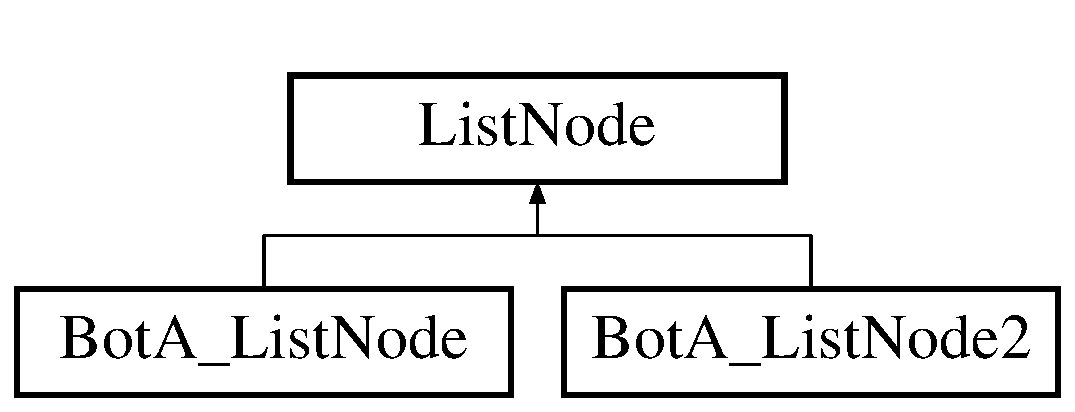
\includegraphics[height=2cm]{classListNode}
\end{center}
\end{figure}
\subsection*{Public Member Functions}
\begin{CompactItemize}
\item 
{\bf ListNode} ({\bf TreeNode} $\ast${\bf treeNode})
\item 
virtual {\bf $\sim$ListNode} ()
\item 
{\bf TreeNode} $\ast$ {\bf getTreeNode} (void) const 
\item 
{\bf ListNode} $\ast$ {\bf getNext} (void) const 
\item 
{\bf ListNode} $\ast$ {\bf getPrev} (void) const 
\item 
{\bf Node} $\ast$ {\bf getNode} (void) const 
\item 
void {\bf setNext} ({\bf ListNode} $\ast${\bf next})
\item 
void {\bf setPrev} ({\bf ListNode} $\ast${\bf prev})
\item 
void {\bf addBefore} ({\bf ListNode} $\ast$listNode)
\item 
void {\bf addAfter} ({\bf ListNode} $\ast$listNode)
\end{CompactItemize}
\subsection*{Protected Attributes}
\begin{CompactItemize}
\item 
{\bf TreeNode} $\ast$ {\bf treeNode}
\item 
{\bf ListNode} $\ast$ {\bf next}
\item 
{\bf ListNode} $\ast$ {\bf prev}
\end{CompactItemize}


\subsection{Detailed Description}
\doxyref{Node}{p.}{classNode} representation for chained lists. 

This \doxyref{ListNode}{p.}{classListNode} contain a \doxyref{TreeNode}{p.}{classTreeNode} with all information about its parent \doxyref{TreeNode}{p.}{classTreeNode} in the processing tree. 

\subsection{Constructor \& Destructor Documentation}
\index{ListNode@{ListNode}!ListNode@{ListNode}}
\index{ListNode@{ListNode}!ListNode@{ListNode}}
\subsubsection{\setlength{\rightskip}{0pt plus 5cm}ListNode::ListNode ({\bf TreeNode} $\ast$ {\em treeNode})}\label{classListNode_3094fb3f7eb3bbcfcfb51b8b3f77e065}


Constructor for empty node \begin{Desc}
\item[Parameters:]
\begin{description}
\item[{\em treeNode}]treeNode to be stocked on this item \end{description}
\end{Desc}
\index{ListNode@{ListNode}!~ListNode@{$\sim$ListNode}}
\index{~ListNode@{$\sim$ListNode}!ListNode@{ListNode}}
\subsubsection{\setlength{\rightskip}{0pt plus 5cm}ListNode::$\sim$ListNode ()\hspace{0.3cm}{\tt  [virtual]}}\label{classListNode_da75c8d715ac609cb7f4a17cac5d4658}


Destructor No destruction of \doxyref{TreeNode}{p.}{classTreeNode} because it will be deleted in it's tree. If treeNode don't belong to a tree anymore when deleting this listNode, then delete it by hand. 

\subsection{Member Function Documentation}
\index{ListNode@{ListNode}!getTreeNode@{getTreeNode}}
\index{getTreeNode@{getTreeNode}!ListNode@{ListNode}}
\subsubsection{\setlength{\rightskip}{0pt plus 5cm}{\bf TreeNode}$\ast$ ListNode::getTreeNode (void) const\hspace{0.3cm}{\tt  [inline]}}\label{classListNode_cadc6e783704c3372fdcdeaa0cddb7a8}


Content \doxyref{TreeNode}{p.}{classTreeNode} with informations about position in the processing tree \index{ListNode@{ListNode}!getNext@{getNext}}
\index{getNext@{getNext}!ListNode@{ListNode}}
\subsubsection{\setlength{\rightskip}{0pt plus 5cm}{\bf ListNode}$\ast$ ListNode::getNext (void) const\hspace{0.3cm}{\tt  [inline]}}\label{classListNode_2c84a9fbd083b5472fb893c0e2a52fc4}


next \doxyref{ListNode}{p.}{classListNode} \index{ListNode@{ListNode}!getPrev@{getPrev}}
\index{getPrev@{getPrev}!ListNode@{ListNode}}
\subsubsection{\setlength{\rightskip}{0pt plus 5cm}{\bf ListNode}$\ast$ ListNode::getPrev (void) const\hspace{0.3cm}{\tt  [inline]}}\label{classListNode_11e82ca85e20a13bcc169165f197bc8d}


previous \doxyref{ListNode}{p.}{classListNode} \index{ListNode@{ListNode}!getNode@{getNode}}
\index{getNode@{getNode}!ListNode@{ListNode}}
\subsubsection{\setlength{\rightskip}{0pt plus 5cm}{\bf Node}$\ast$ ListNode::getNode (void) const\hspace{0.3cm}{\tt  [inline]}}\label{classListNode_83c12c19b7b605c294e6cccbad409f0e}


Content \doxyref{Node}{p.}{classNode} (only light representation of level) \index{ListNode@{ListNode}!setNext@{setNext}}
\index{setNext@{setNext}!ListNode@{ListNode}}
\subsubsection{\setlength{\rightskip}{0pt plus 5cm}void ListNode::setNext ({\bf ListNode} $\ast$ {\em next})\hspace{0.3cm}{\tt  [inline]}}\label{classListNode_3c27820cf91c91c8c6ffce90b848f316}


Assign next \doxyref{ListNode}{p.}{classListNode} \index{ListNode@{ListNode}!setPrev@{setPrev}}
\index{setPrev@{setPrev}!ListNode@{ListNode}}
\subsubsection{\setlength{\rightskip}{0pt plus 5cm}void ListNode::setPrev ({\bf ListNode} $\ast$ {\em prev})\hspace{0.3cm}{\tt  [inline]}}\label{classListNode_e6402f5371159f63334c8f26ffeab40e}


Assign previous \doxyref{ListNode}{p.}{classListNode} \index{ListNode@{ListNode}!addBefore@{addBefore}}
\index{addBefore@{addBefore}!ListNode@{ListNode}}
\subsubsection{\setlength{\rightskip}{0pt plus 5cm}void ListNode::addBefore ({\bf ListNode} $\ast$ {\em listNode})}\label{classListNode_3c18a683c61d6e750aab3bf042a1ac50}


Add a listNode just before this node \begin{Desc}
\item[Parameters:]
\begin{description}
\item[{\em node}]node to add before this node \end{description}
\end{Desc}
\index{ListNode@{ListNode}!addAfter@{addAfter}}
\index{addAfter@{addAfter}!ListNode@{ListNode}}
\subsubsection{\setlength{\rightskip}{0pt plus 5cm}void ListNode::addAfter ({\bf ListNode} $\ast$ {\em listNode})}\label{classListNode_747f265b7e4b0edef2bfbe1a1000dfdd}


Add a listNode just before this node \begin{Desc}
\item[Parameters:]
\begin{description}
\item[{\em node}]node to add after this node \end{description}
\end{Desc}


\subsection{Member Data Documentation}
\index{ListNode@{ListNode}!treeNode@{treeNode}}
\index{treeNode@{treeNode}!ListNode@{ListNode}}
\subsubsection{\setlength{\rightskip}{0pt plus 5cm}{\bf TreeNode}$\ast$ {\bf ListNode::treeNode}\hspace{0.3cm}{\tt  [protected]}}\label{classListNode_67d2ee26507aa9d63530e7c95e578a51}


\doxyref{TreeNode}{p.}{classTreeNode} stocked on this item of the list \index{ListNode@{ListNode}!next@{next}}
\index{next@{next}!ListNode@{ListNode}}
\subsubsection{\setlength{\rightskip}{0pt plus 5cm}{\bf ListNode}$\ast$ {\bf ListNode::next}\hspace{0.3cm}{\tt  [protected]}}\label{classListNode_d78b392c2ddc25c3243d0c2f30692fb1}


Next \doxyref{ListNode}{p.}{classListNode} of the list \index{ListNode@{ListNode}!prev@{prev}}
\index{prev@{prev}!ListNode@{ListNode}}
\subsubsection{\setlength{\rightskip}{0pt plus 5cm}{\bf ListNode}$\ast$ {\bf ListNode::prev}\hspace{0.3cm}{\tt  [protected]}}\label{classListNode_927c9ca1868a6f55ca5c7c2e3e6c0d62}


Previous \doxyref{ListNode}{p.}{classListNode} of the list 

The documentation for this class was generated from the following files:\begin{CompactItemize}
\item 
include/Solver/ListNode.h\item 
src/Solver/ListNode.cpp\end{CompactItemize}

\section{Node Class Reference}
\label{classNode}\index{Node@{Node}}
Lowest representation of a node. Only contain pusher zone and boxes zone.  


{\tt \#include $<$Node.h$>$}

\subsection*{Public Member Functions}
\begin{CompactItemize}
\item 
{\bf Node} (const Solver $\ast${\bf solver})
\item 
{\bf Node} (const Solver $\ast${\bf solver}, {\bf Zone} $\ast${\bf pusherZone}, {\bf Zone} $\ast${\bf boxesZone})
\item 
{\bf Node} (const {\bf Node} $\ast$otherNode)
\item 
{\bf $\sim$Node} ()
\item 
const Solver $\ast$ {\bf getSolver} (void) const 
\item 
{\bf Zone} $\ast$ {\bf getPusherZone} (void) const 
\item 
{\bf Zone} $\ast$ {\bf getBoxesZone} (void) const 
\item 
void {\bf setPusherZone} ({\bf Zone} $\ast${\bf pusherZone})
\item 
void {\bf setBoxesZone} ({\bf Zone} $\ast${\bf boxesZone})
\item 
bool {\bf isEgal} ({\bf Node} $\ast$otherNode) const 
\item 
bool {\bf isSolution} (void) const 
\item 
{\bf Node} $\ast$$\ast$ {\bf findChildren} (void) const 
\item 
Child $\ast$$\ast$ {\bf findMacroChildren} ({\bf Node} $\ast$$\ast$nodeList)
\item 
char $\ast$ {\bf listMovesFromAToB} (const int posA, const int posB) const 
\item 
int {\bf countMovesFromAToB} (const int posA, const int posB) const 
\item 
void {\bf print} (void) const 
\end{CompactItemize}
\subsection*{Protected Member Functions}
\begin{CompactItemize}
\item 
void {\bf dijkstraRec} (int $\ast$levelTab, const int startPos, const int colsNumber) const 
\item 
int $\ast$ {\bf computeCostOfGoals} ({\bf Node} $\ast$node)
\end{CompactItemize}
\subsection*{Protected Attributes}
\begin{CompactItemize}
\item 
const Solver $\ast$ {\bf solver}
\item 
{\bf Zone} $\ast$ {\bf pusherZone}
\item 
{\bf Zone} $\ast$ {\bf boxesZone}
\end{CompactItemize}
\subsection*{Classes}
\begin{CompactItemize}
\item 
class {\bf Macro}
\end{CompactItemize}


\subsection{Detailed Description}
Lowest representation of a node. Only contain pusher zone and boxes zone. 

This is the minimum representation of a level state. But this state cannot be used without the original level 

\subsection{Constructor \& Destructor Documentation}
\index{Node@{Node}!Node@{Node}}
\index{Node@{Node}!Node@{Node}}
\subsubsection{\setlength{\rightskip}{0pt plus 5cm}Node::Node (const Solver $\ast$ {\em solver})}\label{classNode_18da1ba0aa4ae3a68de1b2a50e4d46ce}


Constructor for a empty node assigned to a solver \begin{Desc}
\item[Parameters:]
\begin{description}
\item[{\em solver}]Assigned solver \end{description}
\end{Desc}
\index{Node@{Node}!Node@{Node}}
\index{Node@{Node}!Node@{Node}}
\subsubsection{\setlength{\rightskip}{0pt plus 5cm}Node::Node (const Solver $\ast$ {\em solver}, {\bf Zone} $\ast$ {\em pusherZone}, {\bf Zone} $\ast$ {\em boxesZone})}\label{classNode_42084887a696848731462de80203b3d7}


Constructor for a node with defined pusherZone and boxesZone \begin{Desc}
\item[Parameters:]
\begin{description}
\item[{\em solver}]Assigned solver \item[{\em pusherZone}]zone where pusher can move \item[{\em boxesZone}]zone of boxes positions \end{description}
\end{Desc}
\index{Node@{Node}!Node@{Node}}
\index{Node@{Node}!Node@{Node}}
\subsubsection{\setlength{\rightskip}{0pt plus 5cm}Node::Node (const {\bf Node} $\ast$ {\em otherNode})}\label{classNode_3a5d189805a56b425ce85dac3ecf569e}


Constructor for a node that's copy of another node \begin{Desc}
\item[Parameters:]
\begin{description}
\item[{\em otherNode}]other node we want to copy \end{description}
\end{Desc}
\index{Node@{Node}!~Node@{$\sim$Node}}
\index{~Node@{$\sim$Node}!Node@{Node}}
\subsubsection{\setlength{\rightskip}{0pt plus 5cm}Node::$\sim$Node ()}\label{classNode_a0840c3cb5c7159be6d992adecd2097c}


Destructor 

\subsection{Member Function Documentation}
\index{Node@{Node}!getSolver@{getSolver}}
\index{getSolver@{getSolver}!Node@{Node}}
\subsubsection{\setlength{\rightskip}{0pt plus 5cm}const Solver$\ast$ Node::getSolver (void) const\hspace{0.3cm}{\tt  [inline]}}\label{classNode_efc2b775577b323c9b727f4f1f05a991}


Assigned solver \index{Node@{Node}!getPusherZone@{getPusherZone}}
\index{getPusherZone@{getPusherZone}!Node@{Node}}
\subsubsection{\setlength{\rightskip}{0pt plus 5cm}{\bf Zone}$\ast$ Node::getPusherZone (void) const\hspace{0.3cm}{\tt  [inline]}}\label{classNode_6e8ba21ef67fbe0012318900b7f210aa}


\doxyref{Zone}{p.}{classZone} of possible pusher move \index{Node@{Node}!getBoxesZone@{getBoxesZone}}
\index{getBoxesZone@{getBoxesZone}!Node@{Node}}
\subsubsection{\setlength{\rightskip}{0pt plus 5cm}{\bf Zone}$\ast$ Node::getBoxesZone (void) const\hspace{0.3cm}{\tt  [inline]}}\label{classNode_a2984742e4312653e1403324f6be153c}


\doxyref{Zone}{p.}{classZone} of boxes \index{Node@{Node}!setPusherZone@{setPusherZone}}
\index{setPusherZone@{setPusherZone}!Node@{Node}}
\subsubsection{\setlength{\rightskip}{0pt plus 5cm}void Node::setPusherZone ({\bf Zone} $\ast$ {\em pusherZone})\hspace{0.3cm}{\tt  [inline]}}\label{classNode_46510e71c4cbda1300948d375e188312}


Assign pusher zone \index{Node@{Node}!setBoxesZone@{setBoxesZone}}
\index{setBoxesZone@{setBoxesZone}!Node@{Node}}
\subsubsection{\setlength{\rightskip}{0pt plus 5cm}void Node::setBoxesZone ({\bf Zone} $\ast$ {\em boxesZone})\hspace{0.3cm}{\tt  [inline]}}\label{classNode_0f5a7e37dd3cd17f91e8aa73962a769d}


Assign boxes zone \index{Node@{Node}!isEgal@{isEgal}}
\index{isEgal@{isEgal}!Node@{Node}}
\subsubsection{\setlength{\rightskip}{0pt plus 5cm}bool Node::isEgal ({\bf Node} $\ast$ {\em otherNode}) const}\label{classNode_6d3e8d8b4fba3b2405e69bccfb7e82ea}


Test if this node is egal to another node \begin{Desc}
\item[Parameters:]
\begin{description}
\item[{\em otherNode}]Other node we want to compare to this \doxyref{Node}{p.}{classNode} object WARNING : 2 nodes must provide from the same level ! \end{description}
\end{Desc}
\begin{Desc}
\item[Returns:]true if node is the same, false if not \end{Desc}
\index{Node@{Node}!isSolution@{isSolution}}
\index{isSolution@{isSolution}!Node@{Node}}
\subsubsection{\setlength{\rightskip}{0pt plus 5cm}bool Node::isSolution (void) const}\label{classNode_cb1173c78f7b3b71b45c8281d341234a}


Test if a node is a solution node for the associed level \begin{Desc}
\item[Returns:]true if this node is solution, false if not \end{Desc}
\index{Node@{Node}!findChildren@{findChildren}}
\index{findChildren@{findChildren}!Node@{Node}}
\subsubsection{\setlength{\rightskip}{0pt plus 5cm}{\bf Node} $\ast$$\ast$ Node::findChildren (void) const}\label{classNode_79458fe90f375dc6c23f316bf6f4c72f}


Use this node to find all successor nodes. A successor node exists if it can be reached from the original node just by pushing a box. \begin{Desc}
\item[Returns:]list of all successor nodes. Terminated by a NULL. \end{Desc}
\index{Node@{Node}!findMacroChildren@{findMacroChildren}}
\index{findMacroChildren@{findMacroChildren}!Node@{Node}}
\subsubsection{\setlength{\rightskip}{0pt plus 5cm}Child $\ast$$\ast$ Node::findMacroChildren ({\bf Node} $\ast$$\ast$ {\em nodeList})}\label{classNode_2bc13b438c902d39444d12c7f9670e0e}


Use this node to find all macro successor nodes. A macro successor node exists if we can push a box on a goal directly, even if you have to do many pushes of the same box to make it. \begin{Desc}
\item[Parameters:]
\begin{description}
\item[{\em nodeList}]list of direct successor previously found with findChildren. \end{description}
\end{Desc}
\begin{Desc}
\item[Returns:]modified nodeList added with all macro pushes. Terminated by a NULL. 

tab of number of pushes for all macro-pushes. \end{Desc}
\index{Node@{Node}!listMovesFromAToB@{listMovesFromAToB}}
\index{listMovesFromAToB@{listMovesFromAToB}!Node@{Node}}
\subsubsection{\setlength{\rightskip}{0pt plus 5cm}char $\ast$ Node::listMovesFromAToB (const int {\em posA}, const int {\em posB}) const}\label{classNode_a730f2ec83d1d3d5224cb97cb127e1e7}


This function use this node (box positions) to make the shortest way between position A and position B in the level and return list of moves used to do it. Be carreful, no box can be pushed on the way from A to B \begin{Desc}
\item[Parameters:]
\begin{description}
\item[{\em posA}]starting position (level representation) \item[{\em posB}]ending position (level representation) \end{description}
\end{Desc}
\begin{Desc}
\item[Returns:]list of moves to go from posA to posB terminated by '' \end{Desc}
\index{Node@{Node}!countMovesFromAToB@{countMovesFromAToB}}
\index{countMovesFromAToB@{countMovesFromAToB}!Node@{Node}}
\subsubsection{\setlength{\rightskip}{0pt plus 5cm}int Node::countMovesFromAToB (const int {\em posA}, const int {\em posB}) const}\label{classNode_969627276733f88fc8740b0a54d82478}


This function use this node (box positions) to make the shortest way between position A and position B in the level and return number of moves used to do it. Be carreful, no box can be pushed on the way from A to B \begin{Desc}
\item[Parameters:]
\begin{description}
\item[{\em posA}]starting position (level representation) \item[{\em posB}]ending position (level representation) \end{description}
\end{Desc}
\begin{Desc}
\item[Returns:]number of moves to go from posA to posB. \end{Desc}
\index{Node@{Node}!print@{print}}
\index{print@{print}!Node@{Node}}
\subsubsection{\setlength{\rightskip}{0pt plus 5cm}void Node::print (void) const}\label{classNode_1ff239408f3d6f9e7d9e2b2f378b5150}


Print node (level) state in the console \index{Node@{Node}!dijkstraRec@{dijkstraRec}}
\index{dijkstraRec@{dijkstraRec}!Node@{Node}}
\subsubsection{\setlength{\rightskip}{0pt plus 5cm}void Node::dijkstraRec (int $\ast$ {\em levelTab}, const int {\em startPos}, const int {\em colsNumber}) const\hspace{0.3cm}{\tt  [protected]}}\label{classNode_a4a48cf4b4d6698d255169b3ab8aae84}


Recursive function based on Dijkstra algorithm. It fill a tab in with every informations about min distance between a cell and start pos. \begin{Desc}
\item[Parameters:]
\begin{description}
\item[{\em levelTab}]tab of values (init with -1 for walls and big numbers for every other cells) \item[{\em startPos}]start position to compute (level representation) \item[{\em colsNumber}]number of cols in this level \end{description}
\end{Desc}
\begin{Desc}
\item[Returns:]levelTab filled with every informations about min distances between a cell and start pos \end{Desc}
\index{Node@{Node}!computeCostOfGoals@{computeCostOfGoals}}
\index{computeCostOfGoals@{computeCostOfGoals}!Node@{Node}}
\subsubsection{\setlength{\rightskip}{0pt plus 5cm}int $\ast$ Node::computeCostOfGoals ({\bf Node} $\ast$ {\em node})\hspace{0.3cm}{\tt  [protected]}}\label{classNode_b2cdfdaa1da7b794bee11ac004575c28}


Get cost of every goals for this node. A cost of a goal is the number of boxes or walls just next this goal. cost go from 0 to 4. 4 is a top priority goal \begin{Desc}
\item[Parameters:]
\begin{description}
\item[{\em node}]node to be tested \end{description}
\end{Desc}
\begin{Desc}
\item[Returns:]tab of cost of each goal \end{Desc}


\subsection{Member Data Documentation}
\index{Node@{Node}!solver@{solver}}
\index{solver@{solver}!Node@{Node}}
\subsubsection{\setlength{\rightskip}{0pt plus 5cm}const Solver$\ast$ {\bf Node::solver}\hspace{0.3cm}{\tt  [protected]}}\label{classNode_68847a1ead037b788c4c8d4495ea5f7b}


Assigned solver \index{Node@{Node}!pusherZone@{pusherZone}}
\index{pusherZone@{pusherZone}!Node@{Node}}
\subsubsection{\setlength{\rightskip}{0pt plus 5cm}{\bf Zone}$\ast$ {\bf Node::pusherZone}\hspace{0.3cm}{\tt  [protected]}}\label{classNode_c790ea0a62d0afd78353bb42ab213d93}


Move zone of the pusher \index{Node@{Node}!boxesZone@{boxesZone}}
\index{boxesZone@{boxesZone}!Node@{Node}}
\subsubsection{\setlength{\rightskip}{0pt plus 5cm}{\bf Zone}$\ast$ {\bf Node::boxesZone}\hspace{0.3cm}{\tt  [protected]}}\label{classNode_db218c8805a8f69e1b20e7fc07999d42}


Position of boxes 

The documentation for this class was generated from the following files:\begin{CompactItemize}
\item 
include/Solver/Node.h\item 
src/Solver/Node.cpp\end{CompactItemize}

\section{Node::Macro Class Reference}
\label{classNode_1_1Macro}\index{Node::Macro@{Node::Macro}}
{\tt \#include $<$Node.h$>$}



\subsection{Detailed Description}
Usefull class to store informations on macro-pushes 

The documentation for this class was generated from the following file:\begin{CompactItemize}
\item 
include/Solver/Node.h\end{CompactItemize}

\section{Pack Class Reference}
\label{classPack}\index{Pack@{Pack}}
Class used to store a (xml) pack of levels.  


{\tt \#include $<$Pack.h$>$}

\subsection*{Public Member Functions}
\begin{CompactItemize}
\item 
{\bf Pack} (Base $\ast${\bf base})
\item 
{\bf Pack} (Base $\ast${\bf base}, const char $\ast$xmlPackFile, const char $\ast${\bf player})
\item 
{\bf $\sim$Pack} ()
\item 
const char $\ast$ {\bf getFileName} (void) const 
\item 
const char $\ast$ {\bf getTitle} (void) const 
\item 
const char $\ast$ {\bf getDescription} (void) const 
\item 
const char $\ast$ {\bf getCopyright} (void) const 
\item 
const char $\ast$ {\bf getEmail} (void) const 
\item 
const char $\ast$ {\bf getUrl} (void) const 
\item 
int {\bf getMaxRowsNumber} (void) const 
\item 
int {\bf getMaxColsNumber} (void) const 
\item 
{\bf Level} $\ast$const $\ast$const {\bf getLevelList} (void) const 
\item 
int {\bf getN} (void) const 
\item 
int {\bf getNSuccess} (void) const 
\item 
void {\bf print} (const char $\ast${\bf fileName}) const 
\item 
void {\bf print} (void) const 
\item 
void {\bf xmlSavePath} (void) const 
\end{CompactItemize}
\subsection*{Protected Member Functions}
\begin{CompactItemize}
\item 
void {\bf xmlLoad} (const char $\ast$xmlPackFile, const char $\ast${\bf player})
\item 
xmlNodePtr $\ast$ {\bf xmlLoadLevels} (xmlDocPtr $\ast$tree, const char $\ast$xmlPackFile)
\item 
xmlNodePtr $\ast$ {\bf xmlLoadPath} (xmlDocPtr $\ast$tree, const char $\ast${\bf player}, const char $\ast$xmlPackFile)
\item 
void {\bf printInFile} (const char $\ast${\bf fileName}) const 
\end{CompactItemize}
\subsection*{Protected Attributes}
\begin{CompactItemize}
\item 
Base $\ast$ {\bf base}
\item 
char {\bf fileName} [33]
\item 
char {\bf player} [33]
\item 
char {\bf title} [65]
\item 
char {\bf description} [513]
\item 
char {\bf copyright} [65]
\item 
char {\bf email} [65]
\item 
char {\bf url} [129]
\item 
int {\bf maxRowsNumber}
\item 
int {\bf maxColsNumber}
\item 
{\bf Level} $\ast$$\ast$ {\bf levelList}
\item 
int {\bf n}
\item 
int {\bf nSuccess}
\end{CompactItemize}


\subsection{Detailed Description}
Class used to store a (xml) pack of levels. 

Scores (Paths) associed with these levels are loaded from an external (xml too) file and are relative to loggued player (param to constructor) 

\subsection{Constructor \& Destructor Documentation}
\index{Pack@{Pack}!Pack@{Pack}}
\index{Pack@{Pack}!Pack@{Pack}}
\subsubsection{\setlength{\rightskip}{0pt plus 5cm}Pack::Pack (Base $\ast$ {\em base})}\label{classPack_3160052a36fb984a2bbdef88a890bbb5}


Constructor for a empty pack \begin{Desc}
\item[Parameters:]
\begin{description}
\item[{\em base}]main class of the game \end{description}
\end{Desc}
\index{Pack@{Pack}!Pack@{Pack}}
\index{Pack@{Pack}!Pack@{Pack}}
\subsubsection{\setlength{\rightskip}{0pt plus 5cm}Pack::Pack (Base $\ast$ {\em base}, const char $\ast$ {\em xmlPackFile}, const char $\ast$ {\em player})}\label{classPack_344de883e5366bea4e658b9b2091a3ea}


Constructor for a pack from xml files. One for levels, one for paths (solutions/high scores) \begin{Desc}
\item[Parameters:]
\begin{description}
\item[{\em base}]main class of the game \item[{\em xmlPackFile}]name of the xml file containing a pack of levels situated in data/levels/ \item[{\em player}]name of loggued player (to know paths to load) \end{description}
\end{Desc}
\index{Pack@{Pack}!~Pack@{$\sim$Pack}}
\index{~Pack@{$\sim$Pack}!Pack@{Pack}}
\subsubsection{\setlength{\rightskip}{0pt plus 5cm}Pack::$\sim$Pack ()}\label{classPack_466f437fb0f9deac378aa60f9637baee}


Destructor 

\subsection{Member Function Documentation}
\index{Pack@{Pack}!getFileName@{getFileName}}
\index{getFileName@{getFileName}!Pack@{Pack}}
\subsubsection{\setlength{\rightskip}{0pt plus 5cm}const char$\ast$ Pack::getFileName (void) const\hspace{0.3cm}{\tt  [inline]}}\label{classPack_33bbca165c6f75f07f723efac7c129bc}


name of loaded xml file \index{Pack@{Pack}!getTitle@{getTitle}}
\index{getTitle@{getTitle}!Pack@{Pack}}
\subsubsection{\setlength{\rightskip}{0pt plus 5cm}const char$\ast$ Pack::getTitle (void) const\hspace{0.3cm}{\tt  [inline]}}\label{classPack_02237c558dd96fd2b47785f4d5586a87}


title of the pack \index{Pack@{Pack}!getDescription@{getDescription}}
\index{getDescription@{getDescription}!Pack@{Pack}}
\subsubsection{\setlength{\rightskip}{0pt plus 5cm}const char$\ast$ Pack::getDescription (void) const\hspace{0.3cm}{\tt  [inline]}}\label{classPack_42a519ae289e10ec5553d2bb0d9fc539}


Description of pack \index{Pack@{Pack}!getCopyright@{getCopyright}}
\index{getCopyright@{getCopyright}!Pack@{Pack}}
\subsubsection{\setlength{\rightskip}{0pt plus 5cm}const char$\ast$ Pack::getCopyright (void) const\hspace{0.3cm}{\tt  [inline]}}\label{classPack_6962e2af68918b3518d8cb905dfea4c5}


Copyright of pack \index{Pack@{Pack}!getEmail@{getEmail}}
\index{getEmail@{getEmail}!Pack@{Pack}}
\subsubsection{\setlength{\rightskip}{0pt plus 5cm}const char$\ast$ Pack::getEmail (void) const\hspace{0.3cm}{\tt  [inline]}}\label{classPack_ff645ae0e0ede27e1ec70689166220c8}


Email of pack \index{Pack@{Pack}!getUrl@{getUrl}}
\index{getUrl@{getUrl}!Pack@{Pack}}
\subsubsection{\setlength{\rightskip}{0pt plus 5cm}const char$\ast$ Pack::getUrl (void) const\hspace{0.3cm}{\tt  [inline]}}\label{classPack_57a2df77d2378bdff8c009ec899370cc}


Url of pack \index{Pack@{Pack}!getMaxRowsNumber@{getMaxRowsNumber}}
\index{getMaxRowsNumber@{getMaxRowsNumber}!Pack@{Pack}}
\subsubsection{\setlength{\rightskip}{0pt plus 5cm}int Pack::getMaxRowsNumber (void) const\hspace{0.3cm}{\tt  [inline]}}\label{classPack_b20837563ca73a969f835efcada3a3c3}


max RowsNumber of all loaded levels \index{Pack@{Pack}!getMaxColsNumber@{getMaxColsNumber}}
\index{getMaxColsNumber@{getMaxColsNumber}!Pack@{Pack}}
\subsubsection{\setlength{\rightskip}{0pt plus 5cm}int Pack::getMaxColsNumber (void) const\hspace{0.3cm}{\tt  [inline]}}\label{classPack_93f088d4417fca1c62a1d0e232f31663}


max ColsNumber of all loaded levels \index{Pack@{Pack}!getLevelList@{getLevelList}}
\index{getLevelList@{getLevelList}!Pack@{Pack}}
\subsubsection{\setlength{\rightskip}{0pt plus 5cm}{\bf Level}$\ast$ const$\ast$ const Pack::getLevelList (void) const\hspace{0.3cm}{\tt  [inline]}}\label{classPack_c51a012d73f889da5690a4e0a2c47090}


tab of \char`\"{}n\char`\"{} \doxyref{Level}{p.}{classLevel} pointers \index{Pack@{Pack}!getN@{getN}}
\index{getN@{getN}!Pack@{Pack}}
\subsubsection{\setlength{\rightskip}{0pt plus 5cm}int Pack::getN (void) const\hspace{0.3cm}{\tt  [inline]}}\label{classPack_e2af8bf120d1e7dfeac776094c690c8f}


Number of levels in this pack \index{Pack@{Pack}!getNSuccess@{getNSuccess}}
\index{getNSuccess@{getNSuccess}!Pack@{Pack}}
\subsubsection{\setlength{\rightskip}{0pt plus 5cm}int Pack::getNSuccess (void) const\hspace{0.3cm}{\tt  [inline]}}\label{classPack_62c006c15d03b945ba61563729251703}


Number of successfull levels in this pack \index{Pack@{Pack}!print@{print}}
\index{print@{print}!Pack@{Pack}}
\subsubsection{\setlength{\rightskip}{0pt plus 5cm}void Pack::print (const char $\ast$ {\em fileName}) const}\label{classPack_05963106a1c7e318f97aa78bd3e2aa19}


Print pack of levels in text mode in a file. \begin{Desc}
\item[Parameters:]
\begin{description}
\item[{\em fileName}]name of the file we want to print in. \end{description}
\end{Desc}
\index{Pack@{Pack}!print@{print}}
\index{print@{print}!Pack@{Pack}}
\subsubsection{\setlength{\rightskip}{0pt plus 5cm}void Pack::print (void) const}\label{classPack_a3e21b032e6b530c5a22c377594c327f}


Print pack of levels in standard output \index{Pack@{Pack}!xmlSavePath@{xmlSavePath}}
\index{xmlSavePath@{xmlSavePath}!Pack@{Pack}}
\subsubsection{\setlength{\rightskip}{0pt plus 5cm}void Pack::xmlSavePath (void) const}\label{classPack_56bd1769b4478614a2dfe62e526b1fc8}


Save every paths of every levels in data/profiles/\char`\"{}player\char`\"{}/\char`\"{}pack\char`\"{}.sol \index{Pack@{Pack}!xmlLoad@{xmlLoad}}
\index{xmlLoad@{xmlLoad}!Pack@{Pack}}
\subsubsection{\setlength{\rightskip}{0pt plus 5cm}void Pack::xmlLoad (const char $\ast$ {\em xmlPackFile}, const char $\ast$ {\em player})\hspace{0.3cm}{\tt  [protected]}}\label{classPack_de3d93107f002a3f160ed870ac761b1e}


Open a XML File containing a pack of levels and initialise this object with levels in it \begin{Desc}
\item[Parameters:]
\begin{description}
\item[{\em xmlPackFile}]XML file (with extension) we want to load in path data/levels/ \item[{\em player}]Player we want to load score associated with these levels \end{description}
\end{Desc}
\index{Pack@{Pack}!xmlLoadLevels@{xmlLoadLevels}}
\index{xmlLoadLevels@{xmlLoadLevels}!Pack@{Pack}}
\subsubsection{\setlength{\rightskip}{0pt plus 5cm}xmlNodePtr $\ast$ Pack::xmlLoadLevels (xmlDocPtr $\ast$ {\em tree}, const char $\ast$ {\em xmlPackFile})\hspace{0.3cm}{\tt  [protected]}}\label{classPack_fae542b60d593a7b876b9ed5da93b790}


Create a tree based on a pack xml file and gets nodes related with levels \begin{Desc}
\item[Parameters:]
\begin{description}
\item[{\em xmlPackFile}]XML file (with extension) we want to load in path data/levels/ \end{description}
\end{Desc}
\begin{Desc}
\item[Returns:]tree Tree opened (we return for suppression after work on nodes) 

list of level nodes (terminated with a NULL node) in xml file \end{Desc}
\index{Pack@{Pack}!xmlLoadPath@{xmlLoadPath}}
\index{xmlLoadPath@{xmlLoadPath}!Pack@{Pack}}
\subsubsection{\setlength{\rightskip}{0pt plus 5cm}xmlNodePtr $\ast$ Pack::xmlLoadPath (xmlDocPtr $\ast$ {\em tree}, const char $\ast$ {\em player}, const char $\ast$ {\em xmlPackFile})\hspace{0.3cm}{\tt  [protected]}}\label{classPack_e13af60ba64b088c7446b0420e619bf8}


Create a tree based on a player xml file and gets nodes related with paths \begin{Desc}
\item[Parameters:]
\begin{description}
\item[{\em player}]Player we want to load score associated with these levels \item[{\em xmlPackFile}]XML file (with extension) we want to load in path data/levels/ \end{description}
\end{Desc}
\begin{Desc}
\item[Returns:]tree Tree opened (we return for suppression after work on nodes) 

list of path nodes (terminated with a NULL node) in xml file \end{Desc}
\index{Pack@{Pack}!printInFile@{printInFile}}
\index{printInFile@{printInFile}!Pack@{Pack}}
\subsubsection{\setlength{\rightskip}{0pt plus 5cm}void Pack::printInFile (const char $\ast$ {\em fileName}) const\hspace{0.3cm}{\tt  [protected]}}\label{classPack_ae0c337520f8f7201357777a5d3c28ed}


Print pack of levels in text mode in a file or in the shell. \begin{Desc}
\item[Parameters:]
\begin{description}
\item[{\em fileName}]name of the file we want to print in. If NULL, then it will be print on screen (standard output) \end{description}
\end{Desc}


\subsection{Member Data Documentation}
\index{Pack@{Pack}!base@{base}}
\index{base@{base}!Pack@{Pack}}
\subsubsection{\setlength{\rightskip}{0pt plus 5cm}Base$\ast$ {\bf Pack::base}\hspace{0.3cm}{\tt  [protected]}}\label{classPack_52c22a4115e2d25e5950bd263557fd85}


Main class of the game \index{Pack@{Pack}!fileName@{fileName}}
\index{fileName@{fileName}!Pack@{Pack}}
\subsubsection{\setlength{\rightskip}{0pt plus 5cm}char {\bf Pack::fileName}[33]\hspace{0.3cm}{\tt  [protected]}}\label{classPack_170427e78c276b98ff32602dbf71b2ec}


Name of loaded file \index{Pack@{Pack}!player@{player}}
\index{player@{player}!Pack@{Pack}}
\subsubsection{\setlength{\rightskip}{0pt plus 5cm}char {\bf Pack::player}[33]\hspace{0.3cm}{\tt  [protected]}}\label{classPack_8291d51e05264921e57dfb2e1deef4c6}


Name of player who load pack \index{Pack@{Pack}!title@{title}}
\index{title@{title}!Pack@{Pack}}
\subsubsection{\setlength{\rightskip}{0pt plus 5cm}char {\bf Pack::title}[65]\hspace{0.3cm}{\tt  [protected]}}\label{classPack_313cef310f77e2fe5332071616de9674}


title of pack \index{Pack@{Pack}!description@{description}}
\index{description@{description}!Pack@{Pack}}
\subsubsection{\setlength{\rightskip}{0pt plus 5cm}char {\bf Pack::description}[513]\hspace{0.3cm}{\tt  [protected]}}\label{classPack_798afd9c44360522ed2423c5fe898b5f}


Description of pack \index{Pack@{Pack}!copyright@{copyright}}
\index{copyright@{copyright}!Pack@{Pack}}
\subsubsection{\setlength{\rightskip}{0pt plus 5cm}char {\bf Pack::copyright}[65]\hspace{0.3cm}{\tt  [protected]}}\label{classPack_5523d8b051d539e9e418181e4eddaa17}


Copyright of pack \index{Pack@{Pack}!email@{email}}
\index{email@{email}!Pack@{Pack}}
\subsubsection{\setlength{\rightskip}{0pt plus 5cm}char {\bf Pack::email}[65]\hspace{0.3cm}{\tt  [protected]}}\label{classPack_14d055abca4792efedb4779d14103a30}


email of creator of pack \index{Pack@{Pack}!url@{url}}
\index{url@{url}!Pack@{Pack}}
\subsubsection{\setlength{\rightskip}{0pt plus 5cm}char {\bf Pack::url}[129]\hspace{0.3cm}{\tt  [protected]}}\label{classPack_d16dac9aa9ac34eb5d949f766b10d32f}


url of pack \index{Pack@{Pack}!maxRowsNumber@{maxRowsNumber}}
\index{maxRowsNumber@{maxRowsNumber}!Pack@{Pack}}
\subsubsection{\setlength{\rightskip}{0pt plus 5cm}int {\bf Pack::maxRowsNumber}\hspace{0.3cm}{\tt  [protected]}}\label{classPack_a83855038d58619c72d813f73d8b5e64}


maximum number of rows \index{Pack@{Pack}!maxColsNumber@{maxColsNumber}}
\index{maxColsNumber@{maxColsNumber}!Pack@{Pack}}
\subsubsection{\setlength{\rightskip}{0pt plus 5cm}int {\bf Pack::maxColsNumber}\hspace{0.3cm}{\tt  [protected]}}\label{classPack_0f423632649a026597232319dcac6ac3}


maximum number of cols \index{Pack@{Pack}!levelList@{levelList}}
\index{levelList@{levelList}!Pack@{Pack}}
\subsubsection{\setlength{\rightskip}{0pt plus 5cm}{\bf Level}$\ast$$\ast$ {\bf Pack::levelList}\hspace{0.3cm}{\tt  [protected]}}\label{classPack_a4baf690941d6b3c5beec54cdf2babf1}


List of n objects of \char`\"{}Level$\ast$\char`\"{} type \index{Pack@{Pack}!n@{n}}
\index{n@{n}!Pack@{Pack}}
\subsubsection{\setlength{\rightskip}{0pt plus 5cm}int {\bf Pack::n}\hspace{0.3cm}{\tt  [protected]}}\label{classPack_cf0d5164682b37d4051dcbd1229b8170}


Number of levels in the pack \index{Pack@{Pack}!nSuccess@{nSuccess}}
\index{nSuccess@{nSuccess}!Pack@{Pack}}
\subsubsection{\setlength{\rightskip}{0pt plus 5cm}int {\bf Pack::nSuccess}\hspace{0.3cm}{\tt  [protected]}}\label{classPack_b46d8d7be9d5133b2709fd1fc49cc3ad}


Number of levels successfully complete by loggued player 

The documentation for this class was generated from the following files:\begin{CompactItemize}
\item 
include/Pack.h\item 
src/Pack.cpp\end{CompactItemize}

\section{Path Class Reference}
\label{classPath}\index{Path@{Path}}
Class usefull to represent a way to move in a level.  


{\tt \#include $<$Path.h$>$}

\subsection*{Public Member Functions}
\begin{CompactItemize}
\item 
{\bf Path} (Base $\ast${\bf base})
\item 
{\bf Path} (Base $\ast${\bf base}, const char $\ast$path, const int mode)
\item 
{\bf Path} (Base $\ast${\bf base}, const {\bf Path} $\ast$source)
\item 
{\bf $\sim$Path} ()
\item 
int {\bf getNPushes} (void) const 
\item 
int {\bf getNMoves} (void) const 
\item 
const char $\ast$ {\bf getMoves} (void) const 
\item 
char {\bf getLastMove} (void) const 
\item 
void {\bf addMove} (const char direction)
\item 
void {\bf addPush} (const char direction)
\item 
void {\bf addDisplacement} (const char direction)
\item 
void {\bf deleteLastMove} (void)
\item 
void {\bf print} (void) const 
\end{CompactItemize}
\subsection*{Static Public Member Functions}
\begin{CompactItemize}
\item 
static char $\ast$ {\bf compressPath} (const char $\ast$path)
\item 
static char $\ast$ {\bf uncompressPath} (const char $\ast$path)
\end{CompactItemize}
\subsection*{Static Protected Member Functions}
\begin{CompactItemize}
\item 
static bool {\bf isValidDirection} (const char direction)
\end{CompactItemize}
\subsection*{Protected Attributes}
\begin{CompactItemize}
\item 
Base $\ast$ {\bf base}
\item 
int {\bf nPushes}
\item 
int {\bf nMoves}
\item 
char $\ast$ {\bf moves}
\end{CompactItemize}


\subsection{Detailed Description}
Class usefull to represent a way to move in a level. 

Pushes are represented by upper case and moves by lower case In files, this is writed in COMPRESSED mode, but in this class, it's UNCOMPRESSED for rapidity and flexibility. In compressed mode, when many moves in one direction, letters are prefixed by numbers.

example uncompressed mode : rrrllUUUUUruLLLdlluRRRRdr

example compressed mode : 3r2l5Uru3Ld2lu4Rdr 

\subsection{Constructor \& Destructor Documentation}
\index{Path@{Path}!Path@{Path}}
\index{Path@{Path}!Path@{Path}}
\subsubsection{\setlength{\rightskip}{0pt plus 5cm}Path::Path (Base $\ast$ {\em base})}\label{classPath_65eccf88c5e670906256b4b74a85ec6d}


Constructor for a empty path \begin{Desc}
\item[Parameters:]
\begin{description}
\item[{\em base}]main class of the game \end{description}
\end{Desc}
\index{Path@{Path}!Path@{Path}}
\index{Path@{Path}!Path@{Path}}
\subsubsection{\setlength{\rightskip}{0pt plus 5cm}Path::Path (Base $\ast$ {\em base}, const char $\ast$ {\em path}, const int {\em mode})}\label{classPath_092abfc95b612873cbc1feb27b7075dc}


Constructor with use of a compressed or uncompressed path to start \begin{Desc}
\item[Parameters:]
\begin{description}
\item[{\em base}]main class of the game \item[{\em path}]Compressed or uncompressed path we use to create this object. It's copied and not directly used. \item[{\em mode}]Path::COMPRESSED or Path::UNCOMPRESSED. It depends of \char`\"{}path\char`\"{} style. \end{description}
\end{Desc}
\index{Path@{Path}!Path@{Path}}
\index{Path@{Path}!Path@{Path}}
\subsubsection{\setlength{\rightskip}{0pt plus 5cm}Path::Path (Base $\ast$ {\em base}, const {\bf Path} $\ast$ {\em source})}\label{classPath_ebb9baac215b371e89aba0a8f67d9edf}


Constructor to copy another path in this object \begin{Desc}
\item[Parameters:]
\begin{description}
\item[{\em base}]main class of the game \item[{\em source}]Another path to be copied in this object. It's copied and not directly used. \end{description}
\end{Desc}
\index{Path@{Path}!~Path@{$\sim$Path}}
\index{~Path@{$\sim$Path}!Path@{Path}}
\subsubsection{\setlength{\rightskip}{0pt plus 5cm}Path::$\sim$Path ()}\label{classPath_141da9ff89c85e0ba410b5a73864c267}


Destructor 

\subsection{Member Function Documentation}
\index{Path@{Path}!getNPushes@{getNPushes}}
\index{getNPushes@{getNPushes}!Path@{Path}}
\subsubsection{\setlength{\rightskip}{0pt plus 5cm}int Path::getNPushes (void) const\hspace{0.3cm}{\tt  [inline]}}\label{classPath_f7fd12fc6bacef4589ed6d8b67451e09}


number of pushes \index{Path@{Path}!getNMoves@{getNMoves}}
\index{getNMoves@{getNMoves}!Path@{Path}}
\subsubsection{\setlength{\rightskip}{0pt plus 5cm}int Path::getNMoves (void) const\hspace{0.3cm}{\tt  [inline]}}\label{classPath_d29f1f3e1ca0bc2cab41edb9252edde7}


number of moves \index{Path@{Path}!getMoves@{getMoves}}
\index{getMoves@{getMoves}!Path@{Path}}
\subsubsection{\setlength{\rightskip}{0pt plus 5cm}const char$\ast$ Path::getMoves (void) const\hspace{0.3cm}{\tt  [inline]}}\label{classPath_41dfd561afd9f04fc6f40972d14a6874}


list of moves \index{Path@{Path}!getLastMove@{getLastMove}}
\index{getLastMove@{getLastMove}!Path@{Path}}
\subsubsection{\setlength{\rightskip}{0pt plus 5cm}char Path::getLastMove (void) const\hspace{0.3cm}{\tt  [inline]}}\label{classPath_06167e7c9176cc1f46043724e4f08c40}


direction of last move (l,r,u,d,L,R,U,D) or 'E' if last move does'nt exist \index{Path@{Path}!addMove@{addMove}}
\index{addMove@{addMove}!Path@{Path}}
\subsubsection{\setlength{\rightskip}{0pt plus 5cm}void Path::addMove (const char {\em direction})}\label{classPath_4f7206735beb8634adb509c46434baf8}


Add move in a direction \begin{Desc}
\item[Parameters:]
\begin{description}
\item[{\em direction}]direction where the pusher move \end{description}
\end{Desc}
\index{Path@{Path}!addPush@{addPush}}
\index{addPush@{addPush}!Path@{Path}}
\subsubsection{\setlength{\rightskip}{0pt plus 5cm}void Path::addPush (const char {\em direction})}\label{classPath_ef938e903cc77c0d5ac28e86d54530e6}


Add push in a direction \begin{Desc}
\item[Parameters:]
\begin{description}
\item[{\em direction}]direction where pusher push a box \end{description}
\end{Desc}
\index{Path@{Path}!addDisplacement@{addDisplacement}}
\index{addDisplacement@{addDisplacement}!Path@{Path}}
\subsubsection{\setlength{\rightskip}{0pt plus 5cm}void Path::addDisplacement (const char {\em direction})}\label{classPath_57d5eeb94308f98165b882769f174a53}


Add displacement in a direction. push or move is automatically assigned following of the case of direction \begin{Desc}
\item[Parameters:]
\begin{description}
\item[{\em direction}]direction where pusher push a box \end{description}
\end{Desc}
\index{Path@{Path}!deleteLastMove@{deleteLastMove}}
\index{deleteLastMove@{deleteLastMove}!Path@{Path}}
\subsubsection{\setlength{\rightskip}{0pt plus 5cm}void Path::deleteLastMove (void)}\label{classPath_8a8c820d523b325b7a7c6cd3bf520b85}


Delete last move \index{Path@{Path}!print@{print}}
\index{print@{print}!Path@{Path}}
\subsubsection{\setlength{\rightskip}{0pt plus 5cm}void Path::print (void) const}\label{classPath_b0a785676da270f13d5446915bfe4f40}


Print path of this object \index{Path@{Path}!compressPath@{compressPath}}
\index{compressPath@{compressPath}!Path@{Path}}
\subsubsection{\setlength{\rightskip}{0pt plus 5cm}char $\ast$ Path::compressPath (const char $\ast$ {\em path})\hspace{0.3cm}{\tt  [static]}}\label{classPath_6d1292829656d07b4bf81c5cf672ad38}


Compress a path (see description of \doxyref{Path}{p.}{classPath} class) \begin{Desc}
\item[Parameters:]
\begin{description}
\item[{\em path}]uncompressed path \end{description}
\end{Desc}
\begin{Desc}
\item[Returns:]compressed path \end{Desc}
\index{Path@{Path}!uncompressPath@{uncompressPath}}
\index{uncompressPath@{uncompressPath}!Path@{Path}}
\subsubsection{\setlength{\rightskip}{0pt plus 5cm}char $\ast$ Path::uncompressPath (const char $\ast$ {\em path})\hspace{0.3cm}{\tt  [static]}}\label{classPath_d1622fd253abca97897d7752742121ff}


Uncompress a path (see description of \doxyref{Path}{p.}{classPath} class) \begin{Desc}
\item[Parameters:]
\begin{description}
\item[{\em path}]compressed path \end{description}
\end{Desc}
\begin{Desc}
\item[Returns:]uncompressed path \end{Desc}
\index{Path@{Path}!isValidDirection@{isValidDirection}}
\index{isValidDirection@{isValidDirection}!Path@{Path}}
\subsubsection{\setlength{\rightskip}{0pt plus 5cm}bool Path::isValidDirection (const char {\em direction})\hspace{0.3cm}{\tt  [inline, static, protected]}}\label{classPath_7f1a201c8439b6937f8f6c501e5ff22c}


Is a direction valid (u,d,r,l,U,D,R,L) \begin{Desc}
\item[Parameters:]
\begin{description}
\item[{\em direction}]direction to test \end{description}
\end{Desc}
\begin{Desc}
\item[Returns:]true if valid, false if not \end{Desc}


\subsection{Member Data Documentation}
\index{Path@{Path}!base@{base}}
\index{base@{base}!Path@{Path}}
\subsubsection{\setlength{\rightskip}{0pt plus 5cm}Base$\ast$ {\bf Path::base}\hspace{0.3cm}{\tt  [protected]}}\label{classPath_1be615cbf94866fca99492720a40a2bf}


Main class of the game \index{Path@{Path}!nPushes@{nPushes}}
\index{nPushes@{nPushes}!Path@{Path}}
\subsubsection{\setlength{\rightskip}{0pt plus 5cm}int {\bf Path::nPushes}\hspace{0.3cm}{\tt  [protected]}}\label{classPath_870010c507fb888c3c775698ef325a1f}


Number of pushes \index{Path@{Path}!nMoves@{nMoves}}
\index{nMoves@{nMoves}!Path@{Path}}
\subsubsection{\setlength{\rightskip}{0pt plus 5cm}int {\bf Path::nMoves}\hspace{0.3cm}{\tt  [protected]}}\label{classPath_b8e5d6877c3968adbfbe00797a324e55}


Number of moves \index{Path@{Path}!moves@{moves}}
\index{moves@{moves}!Path@{Path}}
\subsubsection{\setlength{\rightskip}{0pt plus 5cm}char$\ast$ {\bf Path::moves}\hspace{0.3cm}{\tt  [protected]}}\label{classPath_9b9ce3379439b175cbb8b88ab4a69c31}


UNCOMPRESSED List of moves 

The documentation for this class was generated from the following files:\begin{CompactItemize}
\item 
include/Path.h\item 
src/Path.cpp\end{CompactItemize}

\section{StringList Class Reference}
\label{classStringList}\index{StringList@{StringList}}
Management of Lists made of strings.  


{\tt \#include $<$StringList.h$>$}

\subsection*{Public Member Functions}
\begin{CompactItemize}
\item 
{\bf StringList} (Base $\ast${\bf base})
\item 
{\bf StringList} (Base $\ast${\bf base}, const char $\ast$$\ast${\bf list})
\item 
{\bf StringList} (Base $\ast${\bf base}, const {\bf StringList} $\ast${\bf list})
\item 
{\bf StringList} (Base $\ast${\bf base}, const char $\ast$directory)
\item 
{\bf $\sim$StringList} ()
\item 
char $\ast$const $\ast$const {\bf getList} (void) const 
\item 
int {\bf getLength} (void) const 
\item 
void {\bf addString} (const char $\ast$string)
\item 
void {\bf removeString} (const char $\ast$string)
\item 
const char $\ast$ {\bf getString} (int id)
\item 
bool {\bf isPresent} (const char $\ast$string) const 
\item 
void {\bf print} (void) const 
\item 
int {\bf getStringId} (const char $\ast$string) const 
\end{CompactItemize}
\subsection*{Protected Member Functions}
\begin{CompactItemize}
\item 
char $\ast$$\ast$ {\bf fileListing} (const char $\ast$directory) const 
\item 
void {\bf insertList} (char const $\ast$const $\ast${\bf list})
\item 
void {\bf orderList} (void)
\end{CompactItemize}
\subsection*{Protected Attributes}
\begin{CompactItemize}
\item 
Base $\ast$ {\bf base}
\item 
char $\ast$$\ast$ {\bf list}
\item 
int {\bf length}
\end{CompactItemize}


\subsection{Detailed Description}
Management of Lists made of strings. 

Lists are ordred by alphabetical order and don't contain 2 same strings 

\subsection{Constructor \& Destructor Documentation}
\index{StringList@{StringList}!StringList@{StringList}}
\index{StringList@{StringList}!StringList@{StringList}}
\subsubsection{\setlength{\rightskip}{0pt plus 5cm}StringList::StringList (Base $\ast$ {\em base})}\label{classStringList_27f3450aa281ab6706add0ae491a8fd5}


Constructor for a empty list \begin{Desc}
\item[Parameters:]
\begin{description}
\item[{\em base}]main class of the game \end{description}
\end{Desc}
\index{StringList@{StringList}!StringList@{StringList}}
\index{StringList@{StringList}!StringList@{StringList}}
\subsubsection{\setlength{\rightskip}{0pt plus 5cm}StringList::StringList (Base $\ast$ {\em base}, const char $\ast$$\ast$ {\em list})}\label{classStringList_ec444aa29d2d78ce55bfe8af926aef6f}


Constructor for a list based on a tab of strings \begin{Desc}
\item[Parameters:]
\begin{description}
\item[{\em base}]main class of the game \item[{\em list}]List of string. Last string of list must be \char`\"{}.\char`\"{} \end{description}
\end{Desc}
\index{StringList@{StringList}!StringList@{StringList}}
\index{StringList@{StringList}!StringList@{StringList}}
\subsubsection{\setlength{\rightskip}{0pt plus 5cm}StringList::StringList (Base $\ast$ {\em base}, const {\bf StringList} $\ast$ {\em list})}\label{classStringList_126961fc65cb9023e637b71a03c12a5b}


Constructor for a list copied from another list \begin{Desc}
\item[Parameters:]
\begin{description}
\item[{\em base}]main class of the game \item[{\em list}]Another list of string \end{description}
\end{Desc}
\index{StringList@{StringList}!StringList@{StringList}}
\index{StringList@{StringList}!StringList@{StringList}}
\subsubsection{\setlength{\rightskip}{0pt plus 5cm}StringList::StringList (Base $\ast$ {\em base}, const char $\ast$ {\em directory})}\label{classStringList_d41afc751a07197d64f74bb9e4e7a9f0}


Constructor for a list of files contained in a directory \begin{Desc}
\item[Parameters:]
\begin{description}
\item[{\em base}]main class of the game \item[{\em repertory}]repertory we want to list \end{description}
\end{Desc}
\index{StringList@{StringList}!~StringList@{$\sim$StringList}}
\index{~StringList@{$\sim$StringList}!StringList@{StringList}}
\subsubsection{\setlength{\rightskip}{0pt plus 5cm}StringList::$\sim$StringList ()}\label{classStringList_578ccde3ffad1066142964a8f63b609e}


Destructor 

\subsection{Member Function Documentation}
\index{StringList@{StringList}!getList@{getList}}
\index{getList@{getList}!StringList@{StringList}}
\subsubsection{\setlength{\rightskip}{0pt plus 5cm}char$\ast$ const$\ast$ const StringList::getList (void) const\hspace{0.3cm}{\tt  [inline]}}\label{classStringList_4f1002c2e4fc168a4acefb9000cca8a0}


Id of this level \index{StringList@{StringList}!getLength@{getLength}}
\index{getLength@{getLength}!StringList@{StringList}}
\subsubsection{\setlength{\rightskip}{0pt plus 5cm}int StringList::getLength (void) const\hspace{0.3cm}{\tt  [inline]}}\label{classStringList_f4806ee157e0a2f5c657be3cdffa8411}


Name of this level \index{StringList@{StringList}!addString@{addString}}
\index{addString@{addString}!StringList@{StringList}}
\subsubsection{\setlength{\rightskip}{0pt plus 5cm}void StringList::addString (const char $\ast$ {\em string})}\label{classStringList_a09c31af8eed07163aa82f148bed18a5}


Add a element to the list. If this element already exist in the list, it will not be added \begin{Desc}
\item[Parameters:]
\begin{description}
\item[{\em string}]element to add to the list \end{description}
\end{Desc}
\index{StringList@{StringList}!removeString@{removeString}}
\index{removeString@{removeString}!StringList@{StringList}}
\subsubsection{\setlength{\rightskip}{0pt plus 5cm}void StringList::removeString (const char $\ast$ {\em string})}\label{classStringList_93cbcea629bc4e90b64053df0c081bc1}


Remove a element (string) from this list \begin{Desc}
\item[Parameters:]
\begin{description}
\item[{\em string}]element to remove from the list \end{description}
\end{Desc}
\index{StringList@{StringList}!getString@{getString}}
\index{getString@{getString}!StringList@{StringList}}
\subsubsection{\setlength{\rightskip}{0pt plus 5cm}const char $\ast$ StringList::getString (int {\em id})}\label{classStringList_b4302e82856c098ef417bb7e368b4905}


Get a element from the list \begin{Desc}
\item[Parameters:]
\begin{description}
\item[{\em id}]Number of the element to get (starting with 0) \end{description}
\end{Desc}
\begin{Desc}
\item[Returns:]string number \char`\"{}id\char`\"{} from the list \end{Desc}
\index{StringList@{StringList}!isPresent@{isPresent}}
\index{isPresent@{isPresent}!StringList@{StringList}}
\subsubsection{\setlength{\rightskip}{0pt plus 5cm}bool StringList::isPresent (const char $\ast$ {\em string}) const}\label{classStringList_9aab3032d69d1b6fa92c8490cbd516eb}


Is this string present in this list ? Case is not used. So \char`\"{}hello\char`\"{} and \char`\"{}HeLlO\char`\"{} are the same \begin{Desc}
\item[Parameters:]
\begin{description}
\item[{\em string}]string to test \end{description}
\end{Desc}
\begin{Desc}
\item[Returns:]true if present, false if not \end{Desc}
\index{StringList@{StringList}!print@{print}}
\index{print@{print}!StringList@{StringList}}
\subsubsection{\setlength{\rightskip}{0pt plus 5cm}void StringList::print (void) const}\label{classStringList_5935a5cf7dd3792c0f53de6b4c8cc56e}


Print list on standard output \index{StringList@{StringList}!getStringId@{getStringId}}
\index{getStringId@{getStringId}!StringList@{StringList}}
\subsubsection{\setlength{\rightskip}{0pt plus 5cm}int StringList::getStringId (const char $\ast$ {\em string}) const}\label{classStringList_e07361dc2b7266323eb2e3f5f326b471}


Get position of a string on the list \begin{Desc}
\item[Parameters:]
\begin{description}
\item[{\em string}]string we want to find position \end{description}
\end{Desc}
\begin{Desc}
\item[Returns:]position of the string or -1 if not present \end{Desc}
\index{StringList@{StringList}!fileListing@{fileListing}}
\index{fileListing@{fileListing}!StringList@{StringList}}
\subsubsection{\setlength{\rightskip}{0pt plus 5cm}char $\ast$$\ast$ StringList::fileListing (const char $\ast$ {\em directory}) const\hspace{0.3cm}{\tt  [protected]}}\label{classStringList_0b29c0588b3e902d2c621e4d8ac749e7}


List every files in the repertory \char`\"{}rep\char`\"{} \begin{Desc}
\item[Parameters:]
\begin{description}
\item[{\em directory}]Repertory where we want to list files \end{description}
\end{Desc}
\begin{Desc}
\item[Returns:]tab of string where last string is \char`\"{}.\char`\"{} \end{Desc}
\index{StringList@{StringList}!insertList@{insertList}}
\index{insertList@{insertList}!StringList@{StringList}}
\subsubsection{\setlength{\rightskip}{0pt plus 5cm}void StringList::insertList (char const $\ast$const $\ast$ {\em list})\hspace{0.3cm}{\tt  [protected]}}\label{classStringList_77d8eb8324bbb4c49a215793325ad299}


Insert tab of string in this object \begin{Desc}
\item[Parameters:]
\begin{description}
\item[{\em list}]tab of string terminated with string \char`\"{}.\char`\"{} \end{description}
\end{Desc}
\index{StringList@{StringList}!orderList@{orderList}}
\index{orderList@{orderList}!StringList@{StringList}}
\subsubsection{\setlength{\rightskip}{0pt plus 5cm}void StringList::orderList (void)\hspace{0.3cm}{\tt  [protected]}}\label{classStringList_03a8b099db83f072e4a1f3bf413ad00d}


Order this list of string alphabetically 

\subsection{Member Data Documentation}
\index{StringList@{StringList}!base@{base}}
\index{base@{base}!StringList@{StringList}}
\subsubsection{\setlength{\rightskip}{0pt plus 5cm}Base$\ast$ {\bf StringList::base}\hspace{0.3cm}{\tt  [protected]}}\label{classStringList_bcabb0a7b618780433bfaf127aecd8d6}


Main class of the game \index{StringList@{StringList}!list@{list}}
\index{list@{list}!StringList@{StringList}}
\subsubsection{\setlength{\rightskip}{0pt plus 5cm}char$\ast$$\ast$ {\bf StringList::list}\hspace{0.3cm}{\tt  [protected]}}\label{classStringList_5e21265228e4833abd1beed2af452647}


Tab of strings. Final string is a \char`\"{}.\char`\"{} \index{StringList@{StringList}!length@{length}}
\index{length@{length}!StringList@{StringList}}
\subsubsection{\setlength{\rightskip}{0pt plus 5cm}int {\bf StringList::length}\hspace{0.3cm}{\tt  [protected]}}\label{classStringList_8d7fc2f13c6044b760f00e2ced19c6bc}


Length of the string list 

The documentation for this class was generated from the following files:\begin{CompactItemize}
\item 
include/StringList.h\item 
src/StringList.cpp\end{CompactItemize}

\section{TreeNode Class Reference}
\label{classTreeNode}\index{TreeNode@{TreeNode}}
Improved node representation for trees.  


{\tt \#include $<$TreeNode.h$>$}

Inherited by BotA\_\-TreeNode.

\subsection*{Public Member Functions}
\begin{CompactItemize}
\item 
{\bf TreeNode} ({\bf Node} $\ast${\bf node})
\item 
{\bf $\sim$TreeNode} ()
\item 
{\bf Node} $\ast$ {\bf getNode} (void) const 
\item 
{\bf TreeNode} $\ast$ {\bf getParent} (void) const 
\item 
{\bf TreeNode} $\ast$$\ast$ {\bf getChildren} (void) const 
\item 
int {\bf getChildrenNumber} (void) const 
\item 
void {\bf setParent} ({\bf TreeNode} $\ast${\bf parent})
\item 
void {\bf setChildren} ({\bf TreeNode} $\ast$$\ast${\bf children})
\item 
void {\bf setChildrenNumber} (int number)
\item 
void {\bf addChild} ({\bf TreeNode} $\ast$newChild)
\item 
int {\bf getPusherPrePosition} (void) const 
\item 
int {\bf getPusherPosition} (void) const 
\item 
int {\bf getPushedBoxPrePosition} (void) const 
\item 
int {\bf getPushedBoxPostPosition} (void) const 
\item 
int $\ast$ {\bf listOfPusherPositions} (void)
\item 
{\bf Path} $\ast$ {\bf getPath} (void)
\item 
int $\ast$ {\bf computeTreeBoxStats} (int $\ast$statsTab=NULL) const 
\end{CompactItemize}
\subsection*{Protected Attributes}
\begin{CompactItemize}
\item 
{\bf Node} $\ast$ {\bf node}
\item 
{\bf TreeNode} $\ast$ {\bf parent}
\item 
{\bf TreeNode} $\ast$$\ast$ {\bf children}
\item 
int {\bf childrenNumber}
\end{CompactItemize}


\subsection{Detailed Description}
Improved node representation for trees. 

This is the kind of nodes to be used with trees 

\subsection{Constructor \& Destructor Documentation}
\index{TreeNode@{TreeNode}!TreeNode@{TreeNode}}
\index{TreeNode@{TreeNode}!TreeNode@{TreeNode}}
\subsubsection{\setlength{\rightskip}{0pt plus 5cm}TreeNode::TreeNode ({\bf Node} $\ast$ {\em node})}\label{classTreeNode_faa95b5f5b707bf144780f4bd19cc45d}


Constructor for empty node \begin{Desc}
\item[Parameters:]
\begin{description}
\item[{\em node}]\doxyref{Node}{p.}{classNode} to be stocked on this item \end{description}
\end{Desc}
\index{TreeNode@{TreeNode}!~TreeNode@{$\sim$TreeNode}}
\index{~TreeNode@{$\sim$TreeNode}!TreeNode@{TreeNode}}
\subsubsection{\setlength{\rightskip}{0pt plus 5cm}TreeNode::$\sim$TreeNode ()}\label{classTreeNode_138449d182c342d032c78e7037afc151}


Destructor 

\subsection{Member Function Documentation}
\index{TreeNode@{TreeNode}!getNode@{getNode}}
\index{getNode@{getNode}!TreeNode@{TreeNode}}
\subsubsection{\setlength{\rightskip}{0pt plus 5cm}{\bf Node}$\ast$ TreeNode::getNode (void) const\hspace{0.3cm}{\tt  [inline]}}\label{classTreeNode_c551f47b1bc04a1b3ed7d86b3ff76150}


Content node \index{TreeNode@{TreeNode}!getParent@{getParent}}
\index{getParent@{getParent}!TreeNode@{TreeNode}}
\subsubsection{\setlength{\rightskip}{0pt plus 5cm}{\bf TreeNode}$\ast$ TreeNode::getParent (void) const\hspace{0.3cm}{\tt  [inline]}}\label{classTreeNode_00ab2781ab9dec833b2554d17e478bbd}


parent \doxyref{TreeNode}{p.}{classTreeNode} \index{TreeNode@{TreeNode}!getChildren@{getChildren}}
\index{getChildren@{getChildren}!TreeNode@{TreeNode}}
\subsubsection{\setlength{\rightskip}{0pt plus 5cm}{\bf TreeNode}$\ast$$\ast$ TreeNode::getChildren (void) const\hspace{0.3cm}{\tt  [inline]}}\label{classTreeNode_144d4ca2836aa012f640700dab775c05}


tab of children TreeNodes \index{TreeNode@{TreeNode}!getChildrenNumber@{getChildrenNumber}}
\index{getChildrenNumber@{getChildrenNumber}!TreeNode@{TreeNode}}
\subsubsection{\setlength{\rightskip}{0pt plus 5cm}int TreeNode::getChildrenNumber (void) const\hspace{0.3cm}{\tt  [inline]}}\label{classTreeNode_d39f6700a46b5401e12fffaa976c0e9b}


number of children of this \doxyref{TreeNode}{p.}{classTreeNode} \index{TreeNode@{TreeNode}!setParent@{setParent}}
\index{setParent@{setParent}!TreeNode@{TreeNode}}
\subsubsection{\setlength{\rightskip}{0pt plus 5cm}void TreeNode::setParent ({\bf TreeNode} $\ast$ {\em parent})\hspace{0.3cm}{\tt  [inline]}}\label{classTreeNode_e19c26feb50ff57f5e1105ac1f1ebbe7}


Assign parent treeNode \index{TreeNode@{TreeNode}!setChildren@{setChildren}}
\index{setChildren@{setChildren}!TreeNode@{TreeNode}}
\subsubsection{\setlength{\rightskip}{0pt plus 5cm}void TreeNode::setChildren ({\bf TreeNode} $\ast$$\ast$ {\em children})\hspace{0.3cm}{\tt  [inline]}}\label{classTreeNode_1cfa1af14a1449cb111bfd386bd986f1}


Assign tab of children TreeNodes \index{TreeNode@{TreeNode}!setChildrenNumber@{setChildrenNumber}}
\index{setChildrenNumber@{setChildrenNumber}!TreeNode@{TreeNode}}
\subsubsection{\setlength{\rightskip}{0pt plus 5cm}void TreeNode::setChildrenNumber (int {\em number})\hspace{0.3cm}{\tt  [inline]}}\label{classTreeNode_5e2ec156853e8ed33cf8aec044a120f3}


Set children numbers \index{TreeNode@{TreeNode}!addChild@{addChild}}
\index{addChild@{addChild}!TreeNode@{TreeNode}}
\subsubsection{\setlength{\rightskip}{0pt plus 5cm}void TreeNode::addChild ({\bf TreeNode} $\ast$ {\em newChild})}\label{classTreeNode_a9c89e648016a7143383bc8fae476b28}


Add a child node to this node \begin{Desc}
\item[Parameters:]
\begin{description}
\item[{\em newChild}]New child \doxyref{Node}{p.}{classNode} to add to this node \end{description}
\end{Desc}
\index{TreeNode@{TreeNode}!getPusherPrePosition@{getPusherPrePosition}}
\index{getPusherPrePosition@{getPusherPrePosition}!TreeNode@{TreeNode}}
\subsubsection{\setlength{\rightskip}{0pt plus 5cm}int TreeNode::getPusherPrePosition (void) const}\label{classTreeNode_ddc9a818aab9989d1cb05020826d8a55}


Get the \char`\"{}pre\char`\"{} pusher position of this node (cell just before he pushes a box) \begin{Desc}
\item[Returns:]\char`\"{}pre\char`\"{} pusher position (level representation) of this node. return -1 if no pusher preposition (no parent node) \end{Desc}
\index{TreeNode@{TreeNode}!getPusherPosition@{getPusherPosition}}
\index{getPusherPosition@{getPusherPosition}!TreeNode@{TreeNode}}
\subsubsection{\setlength{\rightskip}{0pt plus 5cm}int TreeNode::getPusherPosition (void) const}\label{classTreeNode_057ca53c67b7e9e06aeb1c08e694601f}


Get the pusher position of this node (just after he pushes a box) \begin{Desc}
\item[Returns:]pusher position (level representation) of this node. \end{Desc}
\index{TreeNode@{TreeNode}!getPushedBoxPrePosition@{getPushedBoxPrePosition}}
\index{getPushedBoxPrePosition@{getPushedBoxPrePosition}!TreeNode@{TreeNode}}
\subsubsection{\setlength{\rightskip}{0pt plus 5cm}int TreeNode::getPushedBoxPrePosition (void) const}\label{classTreeNode_6c188a97ae204f3cfa1776de8f120edd}


Get the pushed box pre-position (position of box before it moves) \begin{Desc}
\item[Returns:]pushed box pre-position (level representation) of this node. return -1 if no pushed box (no parent node) \end{Desc}
\index{TreeNode@{TreeNode}!getPushedBoxPostPosition@{getPushedBoxPostPosition}}
\index{getPushedBoxPostPosition@{getPushedBoxPostPosition}!TreeNode@{TreeNode}}
\subsubsection{\setlength{\rightskip}{0pt plus 5cm}int TreeNode::getPushedBoxPostPosition (void) const}\label{classTreeNode_5a58283c669a97d78e9b614d65c9952f}


Get the pushed box post-position (position of box after it moves) \begin{Desc}
\item[Returns:]pushed box post-position (level representation) of this node. return -1 if no pushed box (no parent node) \end{Desc}
\index{TreeNode@{TreeNode}!listOfPusherPositions@{listOfPusherPositions}}
\index{listOfPusherPositions@{listOfPusherPositions}!TreeNode@{TreeNode}}
\subsubsection{\setlength{\rightskip}{0pt plus 5cm}int $\ast$ TreeNode::listOfPusherPositions (void)}\label{classTreeNode_9e350ee4c530c733dabf54e00814b42c}


Return a list of all successive positions of pusher from start treeNode to this node \begin{Desc}
\item[Returns:]list of all successive positions (level representation) of pusher from start treeNode to this node and terminated by \char`\"{}-1\char`\"{} \end{Desc}
\index{TreeNode@{TreeNode}!getPath@{getPath}}
\index{getPath@{getPath}!TreeNode@{TreeNode}}
\subsubsection{\setlength{\rightskip}{0pt plus 5cm}{\bf Path} $\ast$ TreeNode::getPath (void)}\label{classTreeNode_bd52f02d0df87cba8c489f417433a561}


Return path from root of the tree to this treeNode. \begin{Desc}
\item[Returns:]List of moves (\doxyref{Path}{p.}{classPath}) the pusher must do to get this state of level from the root node \end{Desc}
\index{TreeNode@{TreeNode}!computeTreeBoxStats@{computeTreeBoxStats}}
\index{computeTreeBoxStats@{computeTreeBoxStats}!TreeNode@{TreeNode}}
\subsubsection{\setlength{\rightskip}{0pt plus 5cm}int $\ast$ TreeNode::computeTreeBoxStats (int $\ast$ {\em statsTab} = {\tt NULL}) const}\label{classTreeNode_c34ffb29d8582ea48109ffe1473b8fdd}


Compute total num of boxes of this branch for each cell \begin{Desc}
\item[Parameters:]
\begin{description}
\item[{\em statsTab}]must be NULL (usefull to iterative call) \end{description}
\end{Desc}
\begin{Desc}
\item[Returns:]tab of length cells (where length is number of positions where pusher can move) with in each cell total number of box at this position in this branch. \end{Desc}


\subsection{Member Data Documentation}
\index{TreeNode@{TreeNode}!node@{node}}
\index{node@{node}!TreeNode@{TreeNode}}
\subsubsection{\setlength{\rightskip}{0pt plus 5cm}{\bf Node}$\ast$ {\bf TreeNode::node}\hspace{0.3cm}{\tt  [protected]}}\label{classTreeNode_5ab1199f15b0862bc4bd199fe33786f4}


content node of this item in the tree \index{TreeNode@{TreeNode}!parent@{parent}}
\index{parent@{parent}!TreeNode@{TreeNode}}
\subsubsection{\setlength{\rightskip}{0pt plus 5cm}{\bf TreeNode}$\ast$ {\bf TreeNode::parent}\hspace{0.3cm}{\tt  [protected]}}\label{classTreeNode_77ccf52dc11528bf6cff26e9fa857fce}


parent \doxyref{ListNode}{p.}{classListNode} of the tree \index{TreeNode@{TreeNode}!children@{children}}
\index{children@{children}!TreeNode@{TreeNode}}
\subsubsection{\setlength{\rightskip}{0pt plus 5cm}{\bf TreeNode}$\ast$$\ast$ {\bf TreeNode::children}\hspace{0.3cm}{\tt  [protected]}}\label{classTreeNode_12df2f339ab1d109aa0fe21067258ff1}


List of children of the tree \index{TreeNode@{TreeNode}!childrenNumber@{childrenNumber}}
\index{childrenNumber@{childrenNumber}!TreeNode@{TreeNode}}
\subsubsection{\setlength{\rightskip}{0pt plus 5cm}int {\bf TreeNode::childrenNumber}\hspace{0.3cm}{\tt  [protected]}}\label{classTreeNode_bf6e4fe5b27c179bf8fa290d82e517af}


Number of children in the tree 

The documentation for this class was generated from the following files:\begin{CompactItemize}
\item 
include/Solver/TreeNode.h\item 
src/Solver/TreeNode.cpp\end{CompactItemize}

\section{Util Class Reference}
\label{classUtil}\index{Util@{Util}}
Utility class only with static method.  


{\tt \#include $<$Util.h$>$}

\subsection*{Static Public Member Functions}
\begin{CompactItemize}
\item 
static char $\ast$ {\bf cutText} (const char $\ast$text, const int length)
\item 
static char {\bf toUpper} (const char letter)
\item 
static char {\bf toLower} (const char letter)
\item 
static char $\ast$ {\bf stringToLower} (const char $\ast$string)
\item 
static int {\bf numberLength} (const int number)
\item 
static char {\bf nDecimal} (const int number, const int n)
\item 
static bool {\bf isDecimal} (const char a)
\item 
static char $\ast$ {\bf generateRep} (char $\ast$$\ast$reps)
\item 
static void {\bf createRep} (char $\ast$$\ast$reps)
\item 
static bool {\bf isThisFileExists} (char $\ast$file)
\item 
static bool {\bf isThisRepExists} (char $\ast$rep)
\end{CompactItemize}


\subsection{Detailed Description}
Utility class only with static method. 

\subsection{Member Function Documentation}
\index{Util@{Util}!cutText@{cutText}}
\index{cutText@{cutText}!Util@{Util}}
\subsubsection{\setlength{\rightskip}{0pt plus 5cm}char $\ast$ Util::cutText (const char $\ast$ {\em text}, const int {\em length})\hspace{0.3cm}{\tt  [static]}}\label{classUtil_6543bcf3b48e29daf7ce8583ce12f2e4}


Fonction used to cut and clean text and make it ready to draw \begin{Desc}
\item[Parameters:]
\begin{description}
\item[{\em text}]text to be cut \item[{\em length}]max length of the new text \end{description}
\end{Desc}
\begin{Desc}
\item[Returns:]text cut to (max) length chars and cleaned \end{Desc}
\index{Util@{Util}!toUpper@{toUpper}}
\index{toUpper@{toUpper}!Util@{Util}}
\subsubsection{\setlength{\rightskip}{0pt plus 5cm}char Util::toUpper (const char {\em letter})\hspace{0.3cm}{\tt  [static]}}\label{classUtil_714ac4b097bb9b71c100a600558df93e}


Capitalize one char \begin{Desc}
\item[Parameters:]
\begin{description}
\item[{\em letter}]char to capitalize \end{description}
\end{Desc}
\begin{Desc}
\item[Returns:]capitalized char \end{Desc}
\index{Util@{Util}!toLower@{toLower}}
\index{toLower@{toLower}!Util@{Util}}
\subsubsection{\setlength{\rightskip}{0pt plus 5cm}char Util::toLower (const char {\em letter})\hspace{0.3cm}{\tt  [static]}}\label{classUtil_38a875276038938a12f54c446e3ebb52}


Capitalize one char \begin{Desc}
\item[Parameters:]
\begin{description}
\item[{\em letter}]char to UnCapitalize \end{description}
\end{Desc}
\begin{Desc}
\item[Returns:]uncapitalized char \end{Desc}
\index{Util@{Util}!stringToLower@{stringToLower}}
\index{stringToLower@{stringToLower}!Util@{Util}}
\subsubsection{\setlength{\rightskip}{0pt plus 5cm}char $\ast$ Util::stringToLower (const char $\ast$ {\em string})\hspace{0.3cm}{\tt  [static]}}\label{classUtil_3cd22741e64b45f2f68aff09679b9f87}


Uncapitalize one string \begin{Desc}
\item[Parameters:]
\begin{description}
\item[{\em string}]string to UnCapitalize \end{description}
\end{Desc}
\begin{Desc}
\item[Returns:]uncapitalized string \end{Desc}
\index{Util@{Util}!numberLength@{numberLength}}
\index{numberLength@{numberLength}!Util@{Util}}
\subsubsection{\setlength{\rightskip}{0pt plus 5cm}int Util::numberLength (const int {\em number})\hspace{0.3cm}{\tt  [static]}}\label{classUtil_c40d5d12d6feae02fc04b36aafa4d803}


Number of decimals in this number \begin{Desc}
\item[Parameters:]
\begin{description}
\item[{\em number}]number to search in \end{description}
\end{Desc}
\begin{Desc}
\item[Returns:]number of of decimals \end{Desc}
\index{Util@{Util}!nDecimal@{nDecimal}}
\index{nDecimal@{nDecimal}!Util@{Util}}
\subsubsection{\setlength{\rightskip}{0pt plus 5cm}char Util::nDecimal (const int {\em number}, const int {\em n})\hspace{0.3cm}{\tt  [static]}}\label{classUtil_a837bc2354e998a7ff9429bbdf6b2eb4}


Take the Nst decimal in the number \begin{Desc}
\item[Parameters:]
\begin{description}
\item[{\em number}]number to search in \item[{\em n}]number of decimal to return \end{description}
\end{Desc}
\begin{Desc}
\item[Returns:]caracter of the Nst decimal of number \end{Desc}
\index{Util@{Util}!isDecimal@{isDecimal}}
\index{isDecimal@{isDecimal}!Util@{Util}}
\subsubsection{\setlength{\rightskip}{0pt plus 5cm}bool Util::isDecimal (const char {\em a})\hspace{0.3cm}{\tt  [static]}}\label{classUtil_80a8dedaa94e2901a271a304cf665ef0}


Is it a decimal (between 0 and 9) \begin{Desc}
\item[Parameters:]
\begin{description}
\item[{\em a}]caracter to test \end{description}
\end{Desc}
\begin{Desc}
\item[Returns:]true if \char`\"{}a\char`\"{} is a decimal. false if not. \end{Desc}
\index{Util@{Util}!generateRep@{generateRep}}
\index{generateRep@{generateRep}!Util@{Util}}
\subsubsection{\setlength{\rightskip}{0pt plus 5cm}char $\ast$ Util::generateRep (char $\ast$$\ast$ {\em reps})\hspace{0.3cm}{\tt  [static]}}\label{classUtil_449426a320a40a270f6d107f2f6add88}


Generate a one line fileName from a list of repertory Ex : if reps is \char`\"{}file\char`\"{}$|$\char`\"{}name\char`\"{}$|$\char`\"{}michael.pdf\char`\"{}, then a string with \char`\"{}file/name/michael.pdf\char`\"{} will be created. \begin{Desc}
\item[Parameters:]
\begin{description}
\item[{\em rep}]repertories to test. Ends with NUL \end{description}
\end{Desc}
\index{Util@{Util}!createRep@{createRep}}
\index{createRep@{createRep}!Util@{Util}}
\subsubsection{\setlength{\rightskip}{0pt plus 5cm}void Util::createRep (char $\ast$$\ast$ {\em reps})\hspace{0.3cm}{\tt  [static]}}\label{classUtil_bc971ff30f2665d749c4986a952f30e8}


Create a local repertory made by a list of strings. Ex : if reps is \char`\"{}file\char`\"{}$|$\char`\"{}name\char`\"{}$|$\char`\"{}michael\char`\"{}, then a repertory \char`\"{}file/name/michael/\char`\"{} will be created \begin{Desc}
\item[Parameters:]
\begin{description}
\item[{\em rep}]repertories to test. Ends with NULL \end{description}
\end{Desc}
\index{Util@{Util}!isThisFileExists@{isThisFileExists}}
\index{isThisFileExists@{isThisFileExists}!Util@{Util}}
\subsubsection{\setlength{\rightskip}{0pt plus 5cm}bool Util::isThisFileExists (char $\ast$ {\em file})\hspace{0.3cm}{\tt  [static]}}\label{classUtil_891989bed9b632c0dc28834b8787bd9f}


Is this file exists ? \begin{Desc}
\item[Parameters:]
\begin{description}
\item[{\em file}]file to test \end{description}
\end{Desc}
\begin{Desc}
\item[Returns:]true if it exists, false if not \end{Desc}
\index{Util@{Util}!isThisRepExists@{isThisRepExists}}
\index{isThisRepExists@{isThisRepExists}!Util@{Util}}
\subsubsection{\setlength{\rightskip}{0pt plus 5cm}bool Util::isThisRepExists (char $\ast$ {\em rep})\hspace{0.3cm}{\tt  [static]}}\label{classUtil_5e4c6ac30a41e8533bd7fc223d6e4a67}


Is this repertory exists ? \begin{Desc}
\item[Parameters:]
\begin{description}
\item[{\em rep}]repertory to test \end{description}
\end{Desc}
\begin{Desc}
\item[Returns:]true if it exists, false if not \end{Desc}


The documentation for this class was generated from the following files:\begin{CompactItemize}
\item 
include/Util.h\item 
src/Util.cpp\end{CompactItemize}

\section{Zone Class Reference}
\label{classZone}\index{Zone@{Zone}}
Binary representation of positions in a level.  


{\tt \#include $<$Zone.h$>$}

\subsection*{Public Member Functions}
\begin{CompactItemize}
\item 
{\bf Zone} (const {\bf Zone} $\ast${\bf zone})
\item 
{\bf Zone} (FILE $\ast$file, int numberOfPositions)
\item 
{\bf Zone} (int numberOfPositions)
\item 
{\bf Zone} (const {\bf Zone} $\ast$zone1, const {\bf Zone} $\ast$zone2, int operation)
\item 
{\bf Zone} (const {\bf Level} $\ast$level, const int $\ast$levelToZonePos, const int $\ast$zoneToLevelPos, const int {\bf length}, const int operation)
\item 
{\bf Zone} (const {\bf Zone} $\ast$boxes, const int startPos, const int $\ast$levelToZonePos, int colsNumber)
\item 
{\bf $\sim$Zone} ()
\item 
int {\bf getLength} (void) const 
\item 
const unsigned int $\ast$ {\bf getZoneTab} (void) const 
\item 
int {\bf getNumberCell} (void) const 
\item 
void {\bf print} (void) const 
\item 
void {\bf print} (const {\bf Level} $\ast$level, const int $\ast$levelToZonePos) const 
\item 
int {\bf readPos} (const int pos) const 
\item 
void {\bf write1ToPos} (const int pos) const 
\item 
void {\bf write0ToPos} (const int pos) const 
\item 
bool {\bf isEgal} (const {\bf Zone} $\ast$otherZone) const 
\item 
bool {\bf isFullOf0} () const 
\item 
bool {\bf isFullOf1} () const 
\item 
bool {\bf isIncludedIn} (const {\bf Zone} $\ast$anotherZone) const 
\item 
int {\bf getNumberOf1} () const 
\item 
{\bf Zone} $\ast$ {\bf applyOrWith} ({\bf Zone} $\ast$otherZone)
\item 
{\bf Zone} $\ast$ {\bf applyAndWith} ({\bf Zone} $\ast$otherZone)
\item 
{\bf Zone} $\ast$ {\bf applyXorWith} ({\bf Zone} $\ast$otherZone)
\item 
{\bf Zone} $\ast$ {\bf applyNot} ()
\item 
{\bf Zone} $\ast$ {\bf applyMinusWith} ({\bf Zone} $\ast$otherZone)
\item 
void {\bf saveInFile} (FILE $\ast$file)
\end{CompactItemize}
\subsection*{Protected Member Functions}
\begin{CompactItemize}
\item 
void {\bf makeBoxesZone} (const {\bf Level} $\ast$level, const int $\ast$zoneToLevelPos)
\item 
void {\bf makePusherZone} (const {\bf Level} $\ast$level, const int $\ast$levelToZonePos, const int $\ast$zoneToLevelPos)
\item 
void {\bf recursiveMakePusherZone} (const {\bf Zone} $\ast$boxes, const int startPos, const int $\ast$levelToZonePos, const int colsNumber)
\item 
void {\bf makeDeadlockZone} (const {\bf Level} $\ast$level, const int $\ast$levelToZonePos, const int $\ast$zoneToLevelPos)
\item 
void {\bf makeCornerDeadlockZone} (const {\bf Level} $\ast$level, const int $\ast$zoneToLevelPos)
\item 
void {\bf makeLineDeadlockZone} (const {\bf Level} $\ast$level, const int $\ast$levelToZonePos, const int $\ast$zoneToLevelPos)
\item 
void {\bf makeGoalZone} (const {\bf Level} $\ast$level, const int $\ast$zoneToLevelPos)
\item 
void {\bf makeORZone} (const {\bf Zone} $\ast$zone1, const {\bf Zone} $\ast$zone2)
\item 
void {\bf makeANDZone} (const {\bf Zone} $\ast$zone1, const {\bf Zone} $\ast$zone2)
\item 
void {\bf makeXORZone} (const {\bf Zone} $\ast$zone1, const {\bf Zone} $\ast$zone2)
\item 
void {\bf makeNOTZone} (const {\bf Zone} $\ast$zone1)
\item 
void {\bf copyZone} (const {\bf Zone} $\ast$source)
\item 
bool {\bf isInCorner} (const {\bf Level} $\ast$level, const int pos) const 
\end{CompactItemize}
\subsection*{Protected Attributes}
\begin{CompactItemize}
\item 
unsigned int $\ast$ {\bf zone}
\item 
int {\bf length}
\end{CompactItemize}


\subsection{Detailed Description}
Binary representation of positions in a level. 

Can be used to represent boxes zone, pusher move zone, deadlocks zone or goals zone.

\doxyref{Zone}{p.}{classZone} is stocked in a unsigned integer tab (unsigned int = 2 or 4 bits depending of the CPU). Each \char`\"{}usefull\char`\"{} cell of the level (see zoneToLevelPos from solver) corresponds to 1 bit. If this bit is \char`\"{}1\char`\"{} then there is a \char`\"{}box/possible move/deadlock/goal\char`\"{} on this position depending of the wanted action.

Boxes zone representation : 1 if there is a box in this zone position, 0 if not Goals zone representation : 1 if there is a goal in this zone position, 0 if not Deadlock zone representation : 1 if there is a deadlock when a box is in this zone position, 0 if not Pusher move zone representation : 1 if pusher can move on this position OR if this is a box position just next a place where pusher can move, 0 if not 

\subsection{Constructor \& Destructor Documentation}
\index{Zone@{Zone}!Zone@{Zone}}
\index{Zone@{Zone}!Zone@{Zone}}
\subsubsection{\setlength{\rightskip}{0pt plus 5cm}Zone::Zone (const {\bf Zone} $\ast$ {\em zone})}\label{classZone_595bc54882b6d94f0a1184bf848b7174}


Constructor for a zone copied from an existing zone \begin{Desc}
\item[Parameters:]
\begin{description}
\item[{\em zone}]zone we want to copy \end{description}
\end{Desc}
\index{Zone@{Zone}!Zone@{Zone}}
\index{Zone@{Zone}!Zone@{Zone}}
\subsubsection{\setlength{\rightskip}{0pt plus 5cm}Zone::Zone (FILE $\ast$ {\em file}, int {\em numberOfPositions})}\label{classZone_600ce64469f1cbf58d620f5f7dd773cc}


Constructor to create a zone from a opened file \begin{Desc}
\item[Parameters:]
\begin{description}
\item[{\em file}]handle to opened file \item[{\em numberOfPositions}]number of needed positions to store this zone \end{description}
\end{Desc}
\index{Zone@{Zone}!Zone@{Zone}}
\index{Zone@{Zone}!Zone@{Zone}}
\subsubsection{\setlength{\rightskip}{0pt plus 5cm}Zone::Zone (int {\em numberOfPositions})}\label{classZone_e9bb45c3f260c213b013b72871113291}


Constructor to create a zone with a certain number of free positions \begin{Desc}
\item[Parameters:]
\begin{description}
\item[{\em numberOfPositions}]number of needed positions to store this zone \end{description}
\end{Desc}
\index{Zone@{Zone}!Zone@{Zone}}
\index{Zone@{Zone}!Zone@{Zone}}
\subsubsection{\setlength{\rightskip}{0pt plus 5cm}Zone::Zone (const {\bf Zone} $\ast$ {\em zone1}, const {\bf Zone} $\ast$ {\em zone2}, int {\em operation})}\label{classZone_d35bffbeee3126416d7fbbdb5619388f}


Constructor for a zone based on a binary operation on others zones \begin{Desc}
\item[Parameters:]
\begin{description}
\item[{\em zone1}]first zone in binary operation \item[{\em zone2}]second zone in binary operation \item[{\em operation}]Kind of binary operation you want to make : Zone::USE\_\-OR new zone will be the result of an OR operation between zone1 and zone2 Zone::USE\_\-AND new zone will be the result of an AND operation between zone1 and zone2 Zone::USE\_\-XOR new zone will be the result of an XOR operation between zone1 and zone2 Zone::USE NOT new zone will be the result of an NOT operation apply on zone1. zone2 is not used in this case and can be NULL. \end{description}
\end{Desc}
\index{Zone@{Zone}!Zone@{Zone}}
\index{Zone@{Zone}!Zone@{Zone}}
\subsubsection{\setlength{\rightskip}{0pt plus 5cm}Zone::Zone (const {\bf Level} $\ast$ {\em level}, const int $\ast$ {\em levelToZonePos}, const int $\ast$ {\em zoneToLevelPos}, const int {\em length}, const int {\em operation})}\label{classZone_9a4680b877cc4a286be9a334fe43db0b}


Constructor for a zone based on a level state \begin{Desc}
\item[Parameters:]
\begin{description}
\item[{\em level}]original level we want to make zones from it \item[{\em levelToZonePos}]link between real positions and zone positions \item[{\em zoneToLevelPos}]link between zone positions and real positions in the level \item[{\em length}]Number of cells in zoneToLevelPos (number of bits needed) \item[{\em operation}]Kind of zone we want to make : Zone::PROCESS\_\-BOXES if we want to save positions of boxes in the zone Zone::PROCESS\_\-PUSHER if we want to save possibilities of move of the pusher Zone::PROCESS\_\-DEADLOCK if we want to save every places where a deadlock appears if a box is on it. Zone::PROCESS\_\-GOAL if we want to save every goal places \end{description}
\end{Desc}
\index{Zone@{Zone}!Zone@{Zone}}
\index{Zone@{Zone}!Zone@{Zone}}
\subsubsection{\setlength{\rightskip}{0pt plus 5cm}Zone::Zone (const {\bf Zone} $\ast$ {\em boxes}, const int {\em startPos}, const int $\ast$ {\em levelToZonePos}, int {\em colsNumber})}\label{classZone_20b850b82ac29274369b2a614f92252d}


Constructor for pusher zone based on a boxes zone and a starting position \begin{Desc}
\item[Parameters:]
\begin{description}
\item[{\em boxes}]Boxes zone of the level we want to make pusher zone \item[{\em startPos}]Starting position of the pusher (level representation) \item[{\em levelToZonePos}]Link between real positions and zone positions \item[{\em colsNumber}]Number of cols in level \end{description}
\end{Desc}
\index{Zone@{Zone}!~Zone@{$\sim$Zone}}
\index{~Zone@{$\sim$Zone}!Zone@{Zone}}
\subsubsection{\setlength{\rightskip}{0pt plus 5cm}Zone::$\sim$Zone ()}\label{classZone_562607cb5c4120a9316c5e967a5c610b}


Destructor 

\subsection{Member Function Documentation}
\index{Zone@{Zone}!getLength@{getLength}}
\index{getLength@{getLength}!Zone@{Zone}}
\subsubsection{\setlength{\rightskip}{0pt plus 5cm}int Zone::getLength (void) const\hspace{0.3cm}{\tt  [inline]}}\label{classZone_2b0535a445f055b07182053a03cb138e}


Number of positions in the zone \index{Zone@{Zone}!getZoneTab@{getZoneTab}}
\index{getZoneTab@{getZoneTab}!Zone@{Zone}}
\subsubsection{\setlength{\rightskip}{0pt plus 5cm}const unsigned int$\ast$ Zone::getZoneTab (void) const\hspace{0.3cm}{\tt  [inline]}}\label{classZone_3597b21ed9b3e28d5a21125424b5ba8a}


Binary representation of the zone \index{Zone@{Zone}!getNumberCell@{getNumberCell}}
\index{getNumberCell@{getNumberCell}!Zone@{Zone}}
\subsubsection{\setlength{\rightskip}{0pt plus 5cm}int Zone::getNumberCell (void) const\hspace{0.3cm}{\tt  [inline]}}\label{classZone_bc147f33c3c106fab7d5667e33c3ba50}


Calculate number of cells usefull to represent this zone \index{Zone@{Zone}!print@{print}}
\index{print@{print}!Zone@{Zone}}
\subsubsection{\setlength{\rightskip}{0pt plus 5cm}void Zone::print (void) const}\label{classZone_5948d6ad11329da7f6c6d48fbe9cb167}


Print a zone in integer and binary mode \index{Zone@{Zone}!print@{print}}
\index{print@{print}!Zone@{Zone}}
\subsubsection{\setlength{\rightskip}{0pt plus 5cm}void Zone::print (const {\bf Level} $\ast$ {\em level}, const int $\ast$ {\em levelToZonePos}) const}\label{classZone_0908e4e69df5d99cfd369e3ce5f31d60}


Print a zone in its level form \begin{Desc}
\item[Parameters:]
\begin{description}
\item[{\em level}]original level corresponding to the zone \item[{\em levelToZonePos}]Translation table between level and zone \end{description}
\end{Desc}
\index{Zone@{Zone}!readPos@{readPos}}
\index{readPos@{readPos}!Zone@{Zone}}
\subsubsection{\setlength{\rightskip}{0pt plus 5cm}int Zone::readPos (const int {\em pos}) const\hspace{0.3cm}{\tt  [inline]}}\label{classZone_117f797fa5b56658f581dca46eb3d21a}


Read position \char`\"{}pos\char`\"{} of the zone and return 1 or 0 depending of the bit state at this position \begin{Desc}
\item[Parameters:]
\begin{description}
\item[{\em pos}]Position we want to read 0 $<$= pos $<$ NumberCell()$\ast$sizeof(unsigned int) \end{description}
\end{Desc}
\begin{Desc}
\item[Returns:]bit value or -1 if invalid pos \end{Desc}
\index{Zone@{Zone}!write1ToPos@{write1ToPos}}
\index{write1ToPos@{write1ToPos}!Zone@{Zone}}
\subsubsection{\setlength{\rightskip}{0pt plus 5cm}void Zone::write1ToPos (const int {\em pos}) const}\label{classZone_3079c66162f087db9f10cb3c0a97df2b}


Set binary number '1' in the position \char`\"{}pos\char`\"{} of the zone \begin{Desc}
\item[Parameters:]
\begin{description}
\item[{\em pos}]Position where we want to set 1 0 $<$= pos $<$ NumberCell()$\ast$sizeof(unsigned int) \end{description}
\end{Desc}
\index{Zone@{Zone}!write0ToPos@{write0ToPos}}
\index{write0ToPos@{write0ToPos}!Zone@{Zone}}
\subsubsection{\setlength{\rightskip}{0pt plus 5cm}void Zone::write0ToPos (const int {\em pos}) const}\label{classZone_b469d85326ac9096a5501a0d30f36c5c}


Set binary number '0' in the position \char`\"{}pos\char`\"{} of the zone \begin{Desc}
\item[Parameters:]
\begin{description}
\item[{\em pos}]Position where we want to set 1 0 $<$= pos $<$ NumberCell()$\ast$sizeof(unsigned int) \end{description}
\end{Desc}
\index{Zone@{Zone}!isEgal@{isEgal}}
\index{isEgal@{isEgal}!Zone@{Zone}}
\subsubsection{\setlength{\rightskip}{0pt plus 5cm}bool Zone::isEgal (const {\bf Zone} $\ast$ {\em otherZone}) const}\label{classZone_e46007fdce2e005a70f1e3870c8ff69e}


Test if this zone is egal to another zone \begin{Desc}
\item[Parameters:]
\begin{description}
\item[{\em otherZone}]Other zone we want to compare to this \doxyref{Zone}{p.}{classZone} object WARNING : 2 zones must have same lengths ! \end{description}
\end{Desc}
\begin{Desc}
\item[Returns:]true if zone is the same, false if not \end{Desc}
\index{Zone@{Zone}!isFullOf0@{isFullOf0}}
\index{isFullOf0@{isFullOf0}!Zone@{Zone}}
\subsubsection{\setlength{\rightskip}{0pt plus 5cm}bool Zone::isFullOf0 () const}\label{classZone_714a59595d312aaa57231f2ec2aa89cf}


Test if a zone is full of 0 : every bits (and so cells) are egal to 0 \begin{Desc}
\item[Returns:]true if zone is full of 0 \end{Desc}
\index{Zone@{Zone}!isFullOf1@{isFullOf1}}
\index{isFullOf1@{isFullOf1}!Zone@{Zone}}
\subsubsection{\setlength{\rightskip}{0pt plus 5cm}bool Zone::isFullOf1 () const}\label{classZone_671a3b79c2b97088ec6e1a65f5016243}


Test if a zone is full of 1 : every bits are egal to 1 \begin{Desc}
\item[Returns:]true if zone is full of 1 \end{Desc}
\index{Zone@{Zone}!isIncludedIn@{isIncludedIn}}
\index{isIncludedIn@{isIncludedIn}!Zone@{Zone}}
\subsubsection{\setlength{\rightskip}{0pt plus 5cm}bool Zone::isIncludedIn (const {\bf Zone} $\ast$ {\em anotherZone}) const}\label{classZone_1397ccb01645be99161cff98e84fbbe9}


Test if a zone is included in another zone \begin{Desc}
\item[Parameters:]
\begin{description}
\item[{\em anotherZone}]zone where this zone is included or not \end{description}
\end{Desc}
\begin{Desc}
\item[Returns:]true if it's included, false if not \end{Desc}
\index{Zone@{Zone}!getNumberOf1@{getNumberOf1}}
\index{getNumberOf1@{getNumberOf1}!Zone@{Zone}}
\subsubsection{\setlength{\rightskip}{0pt plus 5cm}int Zone::getNumberOf1 () const}\label{classZone_1ce708721d3ee07141bbac29f9fe4fb2}


Return number of 1 in this zone \begin{Desc}
\item[Returns:]number of 1 in this zone \end{Desc}
\index{Zone@{Zone}!applyOrWith@{applyOrWith}}
\index{applyOrWith@{applyOrWith}!Zone@{Zone}}
\subsubsection{\setlength{\rightskip}{0pt plus 5cm}{\bf Zone} $\ast$ Zone::applyOrWith ({\bf Zone} $\ast$ {\em otherZone})}\label{classZone_3530e38a0a99204d4a7c56936974c7cc}


Make a zone representation resulting of a binary operation OR between this zone and the other zone \begin{Desc}
\item[Parameters:]
\begin{description}
\item[{\em otherZone}]\doxyref{Zone}{p.}{classZone} to make binary operation with \end{description}
\end{Desc}
\begin{Desc}
\item[Returns:]resulting zone (this zone that's actually modified) \end{Desc}
\index{Zone@{Zone}!applyAndWith@{applyAndWith}}
\index{applyAndWith@{applyAndWith}!Zone@{Zone}}
\subsubsection{\setlength{\rightskip}{0pt plus 5cm}{\bf Zone} $\ast$ Zone::applyAndWith ({\bf Zone} $\ast$ {\em otherZone})}\label{classZone_7ac8ed17918caf44163a0bc10ff0b51c}


Make a zone representation resulting of a binary operation AND between this zone and the other zone \begin{Desc}
\item[Parameters:]
\begin{description}
\item[{\em otherZone}]\doxyref{Zone}{p.}{classZone} to make binary operation with \end{description}
\end{Desc}
\begin{Desc}
\item[Returns:]resulting zone (this zone that's actually modified) \end{Desc}
\index{Zone@{Zone}!applyXorWith@{applyXorWith}}
\index{applyXorWith@{applyXorWith}!Zone@{Zone}}
\subsubsection{\setlength{\rightskip}{0pt plus 5cm}{\bf Zone} $\ast$ Zone::applyXorWith ({\bf Zone} $\ast$ {\em otherZone})}\label{classZone_0cc9a0b7231c6d44724415b8ed2b841f}


Make a zone representation resulting of a binary operation XOR between this zone and the other zone \begin{Desc}
\item[Parameters:]
\begin{description}
\item[{\em otherZone}]\doxyref{Zone}{p.}{classZone} to make binary operation with \end{description}
\end{Desc}
\begin{Desc}
\item[Returns:]resulting zone (this zone that's actually modified) \end{Desc}
\index{Zone@{Zone}!applyNot@{applyNot}}
\index{applyNot@{applyNot}!Zone@{Zone}}
\subsubsection{\setlength{\rightskip}{0pt plus 5cm}{\bf Zone} $\ast$ Zone::applyNot ()}\label{classZone_687b4ecfa7991810cce547b47c35cc27}


Make a zone representation resulting of a binary operation XOR between this zone and the other zone \begin{Desc}
\item[Returns:]resulting zone (this zone that's actually modified) \end{Desc}
\index{Zone@{Zone}!applyMinusWith@{applyMinusWith}}
\index{applyMinusWith@{applyMinusWith}!Zone@{Zone}}
\subsubsection{\setlength{\rightskip}{0pt plus 5cm}{\bf Zone} $\ast$ Zone::applyMinusWith ({\bf Zone} $\ast$ {\em otherZone})}\label{classZone_3ca3269a31ce68ec94062c6ca19ac7f1}


Make a zone representation resulting of a MINUS binary operation between this zone and the other zone \begin{Desc}
\item[Returns:]resulting zone (this zone that's actually modified) \end{Desc}
\index{Zone@{Zone}!saveInFile@{saveInFile}}
\index{saveInFile@{saveInFile}!Zone@{Zone}}
\subsubsection{\setlength{\rightskip}{0pt plus 5cm}void Zone::saveInFile (FILE $\ast$ {\em file})}\label{classZone_2b4a1a4ff0653ae2af7cf1180d78b014}


Save this zone directly into a file \index{Zone@{Zone}!makeBoxesZone@{makeBoxesZone}}
\index{makeBoxesZone@{makeBoxesZone}!Zone@{Zone}}
\subsubsection{\setlength{\rightskip}{0pt plus 5cm}void Zone::makeBoxesZone (const {\bf Level} $\ast$ {\em level}, const int $\ast$ {\em zoneToLevelPos})\hspace{0.3cm}{\tt  [protected]}}\label{classZone_5fb388d64ff0d460cbbc582d1c084d75}


Make a zone representation of boxes positions in a level \begin{Desc}
\item[Parameters:]
\begin{description}
\item[{\em level}]\doxyref{Level}{p.}{classLevel} we want to make zone \item[{\em zoneToLevelPos}]Link between zone positions and real positions in the level \end{description}
\end{Desc}
\index{Zone@{Zone}!makePusherZone@{makePusherZone}}
\index{makePusherZone@{makePusherZone}!Zone@{Zone}}
\subsubsection{\setlength{\rightskip}{0pt plus 5cm}void Zone::makePusherZone (const {\bf Level} $\ast$ {\em level}, const int $\ast$ {\em levelToZonePos}, const int $\ast$ {\em zoneToLevelPos})\hspace{0.3cm}{\tt  [protected]}}\label{classZone_23384b0021ff0df9b35a418741f6c81e}


Make a zone representation of pusher possible moves in a level \begin{Desc}
\item[Parameters:]
\begin{description}
\item[{\em level}]\doxyref{Level}{p.}{classLevel} we want to make zone \item[{\em levelToZonePos}]Link between level positions and zone positions \item[{\em zoneToLevelPos}]Link between zone positions and real positions in the level \end{description}
\end{Desc}
\index{Zone@{Zone}!recursiveMakePusherZone@{recursiveMakePusherZone}}
\index{recursiveMakePusherZone@{recursiveMakePusherZone}!Zone@{Zone}}
\subsubsection{\setlength{\rightskip}{0pt plus 5cm}void Zone::recursiveMakePusherZone (const {\bf Zone} $\ast$ {\em boxes}, const int {\em startPos}, const int $\ast$ {\em levelToZonePos}, const int {\em colsNumber})\hspace{0.3cm}{\tt  [protected]}}\label{classZone_7a3c83e3ed7422ea767fc93e9d1ee4e4}


Recursively make a zone representation of pusher possible moves in a level \begin{Desc}
\item[Parameters:]
\begin{description}
\item[{\em boxes}]\doxyref{Zone}{p.}{classZone} representation of boxes in this level \item[{\em startPos}]Starting position (level representation) of the pusher \item[{\em levelToZonePos}]Link between level positions and zone positions \item[{\em colsNumber}]Number of cols in level \end{description}
\end{Desc}
\index{Zone@{Zone}!makeDeadlockZone@{makeDeadlockZone}}
\index{makeDeadlockZone@{makeDeadlockZone}!Zone@{Zone}}
\subsubsection{\setlength{\rightskip}{0pt plus 5cm}void Zone::makeDeadlockZone (const {\bf Level} $\ast$ {\em level}, const int $\ast$ {\em levelToZonePos}, const int $\ast$ {\em zoneToLevelPos})\hspace{0.3cm}{\tt  [protected]}}\label{classZone_4e9fdbc9daab3bbda6d8c9b75a2fd04d}


Make a zone representation of places where deadlocks appear if a box is on it \begin{Desc}
\item[Parameters:]
\begin{description}
\item[{\em level}]\doxyref{Level}{p.}{classLevel} we want to make zone \item[{\em levelToZonePos}]Link between level positions and zone positions \item[{\em zoneToLevelPos}]Link between zone positions and real positions in the level \end{description}
\end{Desc}
\index{Zone@{Zone}!makeCornerDeadlockZone@{makeCornerDeadlockZone}}
\index{makeCornerDeadlockZone@{makeCornerDeadlockZone}!Zone@{Zone}}
\subsubsection{\setlength{\rightskip}{0pt plus 5cm}void Zone::makeCornerDeadlockZone (const {\bf Level} $\ast$ {\em level}, const int $\ast$ {\em zoneToLevelPos})\hspace{0.3cm}{\tt  [protected]}}\label{classZone_0a3508a2f32543d96a1e3f134ab8a292}


This function add corner deadlocks to deadlock zone. This happened when there is a box in a corner made by walls \begin{Desc}
\item[Parameters:]
\begin{description}
\item[{\em level}]\doxyref{Level}{p.}{classLevel} we want to make zone \item[{\em zoneToLevelPos}]Link between zone positions and real positions in the level \end{description}
\end{Desc}
\index{Zone@{Zone}!makeLineDeadlockZone@{makeLineDeadlockZone}}
\index{makeLineDeadlockZone@{makeLineDeadlockZone}!Zone@{Zone}}
\subsubsection{\setlength{\rightskip}{0pt plus 5cm}void Zone::makeLineDeadlockZone (const {\bf Level} $\ast$ {\em level}, const int $\ast$ {\em levelToZonePos}, const int $\ast$ {\em zoneToLevelPos})\hspace{0.3cm}{\tt  [protected]}}\label{classZone_dd0a47a68ad20ef2d04c149275c00a36}


This function add line deadlocks to deadlock zone. This happened when there is a box next a wall and no way to remove it (escape move) You must apply this function AFTER the use of function makeCornerDeadlockZone because we need corner positions. \begin{Desc}
\item[Parameters:]
\begin{description}
\item[{\em level}]\doxyref{Level}{p.}{classLevel} we want to make zone \item[{\em levelToZonePos}]Link between level positions and zone positions \item[{\em zoneToLevelPos}]Link between zone positions and real positions in the level \end{description}
\end{Desc}
\index{Zone@{Zone}!makeGoalZone@{makeGoalZone}}
\index{makeGoalZone@{makeGoalZone}!Zone@{Zone}}
\subsubsection{\setlength{\rightskip}{0pt plus 5cm}void Zone::makeGoalZone (const {\bf Level} $\ast$ {\em level}, const int $\ast$ {\em zoneToLevelPos})\hspace{0.3cm}{\tt  [protected]}}\label{classZone_391e4c1403bc1fceb4c1a95babe00c94}


Make a zone representation of goal places \begin{Desc}
\item[Parameters:]
\begin{description}
\item[{\em level}]\doxyref{Level}{p.}{classLevel} we want to make zone \item[{\em zoneToLevelPos}]Link between zone positions and real positions in the level \end{description}
\end{Desc}
\index{Zone@{Zone}!makeORZone@{makeORZone}}
\index{makeORZone@{makeORZone}!Zone@{Zone}}
\subsubsection{\setlength{\rightskip}{0pt plus 5cm}void Zone::makeORZone (const {\bf Zone} $\ast$ {\em zone1}, const {\bf Zone} $\ast$ {\em zone2})\hspace{0.3cm}{\tt  [protected]}}\label{classZone_48bfbd3e0c36b1bb368f847371990c54}


Make a zone representation resulting of a binary operation OR \begin{Desc}
\item[Parameters:]
\begin{description}
\item[{\em zone1}]first zone in binary operation \item[{\em zone2}]second zone in binary operation \end{description}
\end{Desc}
\index{Zone@{Zone}!makeANDZone@{makeANDZone}}
\index{makeANDZone@{makeANDZone}!Zone@{Zone}}
\subsubsection{\setlength{\rightskip}{0pt plus 5cm}void Zone::makeANDZone (const {\bf Zone} $\ast$ {\em zone1}, const {\bf Zone} $\ast$ {\em zone2})\hspace{0.3cm}{\tt  [protected]}}\label{classZone_8038d1df3cbedcba1a876ace75f98d93}


Make a zone representation resulting of a binary operation AND \begin{Desc}
\item[Parameters:]
\begin{description}
\item[{\em zone1}]first zone in binary operation \item[{\em zone2}]second zone in binary operation \end{description}
\end{Desc}
\index{Zone@{Zone}!makeXORZone@{makeXORZone}}
\index{makeXORZone@{makeXORZone}!Zone@{Zone}}
\subsubsection{\setlength{\rightskip}{0pt plus 5cm}void Zone::makeXORZone (const {\bf Zone} $\ast$ {\em zone1}, const {\bf Zone} $\ast$ {\em zone2})\hspace{0.3cm}{\tt  [protected]}}\label{classZone_122eefc299c4a3dcf2946ad7a45e6141}


Make a zone representation resulting of a binary operation XOR \begin{Desc}
\item[Parameters:]
\begin{description}
\item[{\em zone1}]first zone in binary operation \item[{\em zone2}]second zone in binary operation \end{description}
\end{Desc}
\index{Zone@{Zone}!makeNOTZone@{makeNOTZone}}
\index{makeNOTZone@{makeNOTZone}!Zone@{Zone}}
\subsubsection{\setlength{\rightskip}{0pt plus 5cm}void Zone::makeNOTZone (const {\bf Zone} $\ast$ {\em zone1})\hspace{0.3cm}{\tt  [protected]}}\label{classZone_f2833e539189382deaec4b17f04c9127}


Make a zone representation resulting of a binary operation NOT \begin{Desc}
\item[Parameters:]
\begin{description}
\item[{\em zone1}]first zone in binary operation \end{description}
\end{Desc}
\index{Zone@{Zone}!copyZone@{copyZone}}
\index{copyZone@{copyZone}!Zone@{Zone}}
\subsubsection{\setlength{\rightskip}{0pt plus 5cm}void Zone::copyZone (const {\bf Zone} $\ast$ {\em source})\hspace{0.3cm}{\tt  [protected]}}\label{classZone_01ede35498a56be07a4de1fe216a41fe}


Copy other zone in this object. Used by constructor. \begin{Desc}
\item[Parameters:]
\begin{description}
\item[{\em source}]zone to be copied in this object. \end{description}
\end{Desc}
\index{Zone@{Zone}!isInCorner@{isInCorner}}
\index{isInCorner@{isInCorner}!Zone@{Zone}}
\subsubsection{\setlength{\rightskip}{0pt plus 5cm}bool Zone::isInCorner (const {\bf Level} $\ast$ {\em level}, const int {\em pos}) const\hspace{0.3cm}{\tt  [protected]}}\label{classZone_9fd32f0f497111930ed662def90986f5}


return true if position is in a corner of level (corner with 2 walls) \begin{Desc}
\item[Parameters:]
\begin{description}
\item[{\em level}]\doxyref{Level}{p.}{classLevel} we want to test \item[{\em pos}]Position we want to test in the level \end{description}
\end{Desc}
\begin{Desc}
\item[Returns:]true if pos is in a corner of level, return false if not \end{Desc}


\subsection{Member Data Documentation}
\index{Zone@{Zone}!zone@{zone}}
\index{zone@{zone}!Zone@{Zone}}
\subsubsection{\setlength{\rightskip}{0pt plus 5cm}unsigned int$\ast$ {\bf Zone::zone}\hspace{0.3cm}{\tt  [protected]}}\label{classZone_bdd6e8deebb81352f9c7c6bb4674bfe4}


binary representation of the zone \index{Zone@{Zone}!length@{length}}
\index{length@{length}!Zone@{Zone}}
\subsubsection{\setlength{\rightskip}{0pt plus 5cm}int {\bf Zone::length}\hspace{0.3cm}{\tt  [protected]}}\label{classZone_ee37b1a515e2ddd892f8611e0cb023f0}


Number of positions in the zone 

The documentation for this class was generated from the following files:\begin{CompactItemize}
\item 
include/Solver/Zone.h\item 
src/Solver/Zone.cpp\end{CompactItemize}

\printindex
\end{document}
